\documentclass[11pt]{amsart} 
% \usepackage[latin1]{inputenc}
\usepackage[british]{babel}
\usepackage[all]{xy}
\usepackage{amscd}
\usepackage{amssymb}
\usepackage{amsthm}
\usepackage{enumitem}
\usepackage{mathrsfs,bbm}
\usepackage{xcolor,graphicx}
\usepackage{graphics}
\usepackage{soul}
\usepackage{comment}
\usepackage[all]{xy}
\usepackage{amscd}
\usepackage{amssymb,amsmath,latexsym}
\usepackage{amsthm}
\usepackage{enumitem}
\usepackage{mathrsfs,bbm}
\usepackage{dsfont}
\usepackage{tikz-cd}
\usepackage[T1]{fontenc}
\usepackage[utf8]{inputenc}  
 %
%%%%%%%%%%%%%%%%%%%%%%%%%%%%%%%%%%
%pagestyle
%%%%%%%%%%%%%%%%%%%%%%%%%%%%%%%%%%
%\pagestyle{plain}
\textwidth=430pt
\headsep=.7cm
\evensidemargin=15pt
\oddsidemargin=15pt
\leftmargin=0cm
\rightmargin=0cm
%%
%%%%%%%%%%%%%%%%%%%%%%%
\newcommand*\fixitem {\item[]%
  \refstepcounter{enumi}\hskip-\leftmargin\labelenumi\hskip\labelsep}
\newtheorem*{mainthm}{Main Theorem}
\newtheorem*{mainthm1}{Theorem}
\newtheorem*{maincor}{Corollary}
\usepackage[colorlinks=true]{hyperref}
\DeclareMathOperator{\Forall}{\forall}
\DeclareMathOperator{\Exists}{\exists}
\DeclareMathOperator{\ord}{ord}
\newcommand{\phiD}{\varphi_D}
\newcommand{\phiDI}{\varphi_{\mathbf{D}_I}}
\newcommand{\phiDIj}{\varphi_{\mathbf{D}_I (j)}}
\newcommand{\phiH}{\varphi_H}
\newcommand{\phiTimes}{\phiD \otimes \phiH}
\newcommand{\phiTimesDI}{\varphi_{\mathbf{D}_I} \otimes \phiH}
\newcommand{\R}{\mathscr{A}}
\newcommand{\X}{\mathscr{X}}
\newcommand{\Xf}{\mathscr{X}_{(k_0 ,i)}[r_0]}
\newcommand{\Xfr}{\mathscr{X}_{(k_0,i)}[r]}
\newcommand{\hotimes}{\widehat{\otimes}}
\newcommand{\C}{\mathbb{C}_p}
\newcommand{\V}{\mathscr{V}}
\newcommand{\B}{\mathscr{B}}
\newcommand{\dualD}{\mathfrak{D}}
\newcommand{\Dg}{\mathbf{D}}
\newcommand{\DD}{\mathcal{D}^0}
\newcommand{\DDg}{\mathcal{D}}
\newcommand{\DV}{\mathcal{D}}
\newcommand{\W}{\mathscr{W}_N}
\newcommand{\Ao}{\mathbf{A}^\circ}
\newcommand{\AoK}{\mathbf{A}^\circ_{\K}}
\newcommand{\AK}{\mathbf{A}_{/\K}}
\newcommand{\OOO}{\mathscr{A}^\circ}
\newcommand{\K}{\mathcal{K}} 
\newcommand{\OK}{\mathcal{O}_{\K}}
\newcommand{\varprojlog}[1]{\underleftarrow{\log\!^{#1}}}
\newcommand{\T}{\mathscr{T}}
\newcommand{\TT}{\mathbf{T}}
\newcommand{\VV}{\mathbf{V}}
\newcommand{\HH}{\mathcal{H}}
\newcommand{\hh}{\mathcal{H}^+}
\newcommand{\HG}[2]{\mathcal{H}_{#1}(#2)}
\newcommand{\hhl}{\mathcal{H}^{+,[l]}}
\newcommand{\hhj}{\mathcal{H}^{+,[j]}}
\newcommand{\hhjj}{\mathcal{H}^{+,[l,l']}}
\newcommand{\GS}{G_{\mathbb{Q},S}}
\newcommand{\Rf}{R_{(k_0 ,i)}[r_0]}
\newcommand{\Rfr}{R_{(k_0 ,i)}[r]}
\newcommand{\parT}{\langle T\rangle}
\newcommand{\Zf}{Z_{(k_0 ,i)}[r_0]}
\newcommand{\Zfr}{\mathscr{Z}_{(k_0 ,i)}[r]}
\newcommand{\ZFf}{\mathscr{Z}_{(k_0 ,i)}[r_0]}
\newcommand{\ZFfr}{\mathscr{Z}_{(k_0 ,i)}[r]}
\newcommand{\ZF}{\mathscr{Z}}


\title[Fundamental theorem of trop. diff. algebra over nontrivially valued fields]{The Fundamental theorem of tropical differential algebra over nontrivially valued fields and the radius of convergence of nonarchimedean differential equations}

\author{Stefano Mereta}
\email{mereta@kth.se}
\address{KTH Royal Institute of Technology, Brinellvägen 8, 114 28 Stockholm, Sweden}
\author{Francesco Gallinaro}
\email{francesco.gallinaro@mathematik.uni-freiburg.de}
\address{Mathematisches Institut, Albert-Ludwigs-Universität Freiburg, Ernst-Zermelo-Strasse 1, 79104 Freiburg, Germany}

\date{\today}

\subjclass[2010]{Primary 14A20;
	Secondary 12H99, 12H25, 13N99, 14T05, 14T99}
\keywords{tropical geometry; algebraic differential equations; tropical differential equations; $p$-adic differential equations, idempotent semirings, fundamental theorem}

\begin{document}
	\begin{abstract}
        We prove a fundamental theorem for tropical
        partial differential equations analogue of the fundamental theorem of tropical geometry in this context. We extend results from Aroca et al., Falkensteiner et al. and from Fink and Toghani, which work only in the case of trivial valuation as introduced by Grigoriev, to differential equations with power series coefficients over any valued field. To do so, a crucial ingredient is the framework for tropical partial differential equations introduced by Giansiracusa and Mereta. Using this framework we also add a fourth statement to the fundamental theorem, seeing the tropicalization as the set of evaluations of points of the differential Berkovich analytification on the generators of a differential algebra for a given presentation. Lastly, as a corollary of the fundamental theorem, we have that the radius of convergence of solutions of an ordinary differential equation over a nontrivially valued field can be computed tropically.
	\end{abstract}
	\maketitle
	% \tableofcontents
 
\setcounter{tocdepth}{1}	
\tableofcontents

\section*{Introduction}

 Differential equations are ubiquitous in the sciences from theoretical physics to ecology. While a great number of analytical and numerical methods to compute their solutions have been developed since Newton, purely algebraic methods are more recent and generally less developed. The last decade have seen a resurgence of interest in this topic. The theory is based mostly on the pioneering work of Ritt \cite{ritt} and Kolchin \cite{kolchin} on the development of differential algebra, that allows to study systems of algebraic ordinary (and partial) differential equations by means of algebraic tools, such as Gröbner bases, and the works of Macaulay and later Gröbner \cite{grobmac} on the use of differential operators in commutative algebra. This led to the implementation of software routines computing the symbolic solutions of system of linear PDEs (see for example \cite{ridamarc}, \cite{YaironMac}).
 
Algebraic (partial) differential equations are formed from polynomial expressions in an
indeterminate function $f$ and its (partial) derivatives. This smaller class of equations has important applications in the natural sciences, such as
chemical reaction networks, and in pure mathematics where they appear in many parts of geometry. 

Tropical geometry is a fairly new area of algebraic geometry that started developing from the early 2000's and allows to move problems of algebro-geometric nature to a piecewise linear setting  via a valuation. Here methods from combinatorics and polyhedral geometry can be applied to study properties of the initial object. A comprehensive reference for tropical geometry is \cite{macsturm}. 





Tropical methods for algebraic differential equations were introduced for the first time in \cite{grig}. In that paper, the author defined tropical differential equations, their solutions, and a framework for tropicalizing algebraic ODEs over a ring of formal power series $\pk$, and their solutions. The field $K$ is endowed with the trivial valuation. In this context, one tropicalizes differential equations by recording the $t$-adic valuation
of each coefficient, and the tropicalization of power series solutions is performed by applying the trivial valuation of $K$ coefficientwise, i.e. recording their support. The same can also be adapted to the case of PDEs. 
Note that, when $K$ can be endowed with a nontrivial nonarchimedean valuation, Grigoriev's tropicalization does not record any information about the valuation of the coefficients in a differential equation or a power series solution.  Thus all the information about convergence of power series solutions is lost.

In order to remedy this flaw and preserve finer information about the coefficients, in \cite{gianmereta} the authors abstracted the main features of Grigoriev's setting and introduced a framework that extends and refines it. This allows one to perform a tropicalization that, in case the field $K$ has a non-trivial valuation (for example $K$ being the field of Puiseux series or that of $p$-adic numbers) preserves the valuation of the coefficients of the solutions and of the equations. While in the aformentioned paper only results for ODEs are presented, a general framework for PDEs can also be developed, see \cite{tesimereta}. It is in this framework that we will phrase our results, always making clear how these look in the case of ODEs.

Analogously to the fundamental theorem of tropical geometry \cite[Theorem 3.2.3]{macsturm} (also called Kapranov's theorem in the case of hypersurfaces, see \cite{kapranov}), one can ask if solutions to a differential equation tropicalize to solutions of its tropicalization, and if all the tropical solutions can be lifted back. For Grigoriev's setting this question has  been positively answered in the case of ODEs by Aroca et
al.~in \cite{aroca} and subsequently generalised to PDEs in \cite{sebastian} (assuming $K$ is an uncountable algebraically closed field of
characteristic 0). Furthermore, paralleling the role of Gr{\"o}bner theory in the non-differential setting, where a tropical variety is the set of weight vectors whose initial ideal does not contain any monomial, the authors of \cite{FT20} and \cite{hugao} define initial forms and develop a Gr{\"o}bner-theoretic approach to Grigoriev's framework for ODEs. 

In tropical geometry the necessary datum to perform the tropicalization of a set of polynomial equations over a ring $R$ and of its solutions is that of a nonarchimedean valuation $v:R \rightarrow S$ to a semiring $S$. To introduce a similar notion of tropicalization in the differential case we will treat here, we need a \emph{differential enhancement} of such a valuation, see Definition \ref{def:diff-enhan}. For now, let us just say that if $R$ is a differential ring and $v: R \rightarrow S$ is a valuation then a differential enhancement of $v$ is a pair $\mathbf{v}=(v,\widetilde{v})$ where $\widetilde{v}$ is a map from $R$ to a space endowed with a differential structure that is somehow compatible with $v$. 

The main example is roughly the following one (see Section \ref{section:tropdiffeq} for the details). Let $R$ denote the power series ring $\pkk m$, where $K$ is a valued field with value group $\Gamma_K$. Refining \cite{sebastian}, we will introduce a valuation $v$ on $R$ which takes values in a semiring $\textup{Conv}_m(\Gamma_K\cup\{\infty\})$, whose elements are convex hulls  of certain subsets of $\N^m$ with vertices weighted in $\Gamma_K$. We obtain a differential enhancement of $\mathbf v =(v, \widetilde v)$ by taking $\widetilde v$ to be a map from $R$ into a ring of formal power series with coefficients in $\Gamma_K \cup \{\infty\}$, so that the diagram 
\begin{center}
\begin{tikzcd}
& (\Gamma_K \cup \{ \infty \}) [\![t_1 , \dots , t_m]\!]  \arrow[d]  \\
R \arrow[ur, "\widetilde{v}"] \arrow[r, swap, "v"] &  \textup{Conv}_m(\Gamma_K\cup\{\infty\})
\end{tikzcd}
\end{center}
commutes, where the vertical arrow is defined by taking the weighted convex hull of the support of a series. We will tropicalize equations by means of $v$ and solutions via $\widetilde v$. The vertical arrow in the diagram above is a tropical pair, as introduced in \cite{gianmereta}, that we will denote as $\mathbf{\Gamma}_m$.

Furthermore, given a differential algebra $A$ over $R$ and fixing the differential enhancement $\mathbf v$ above, we can consider the set $\textit{Berk}_{\mathbf \Gamma _m}(A)$ of differential enhancements on $A$ extending the one on $R$, as introduced in \cite{gianmereta}. This is a differential analogue of the Berkovich analytification of $A$ and injectively maps to it. 

One of the contributions of the present work is the generalization of the theory developed in \cite{FT20, hugao} to the nontrivially valued case and to PDEs. In this case, the initial form of a differential polynomial with coefficients in $\pkk m $ will depend on a weight vector of tropical power series and on a vector $\omega \in \R^m$ with rationally independent coordinates, and the reason is that in the process of defining the initial form we will make use of the field of multivariate Laurent series with respect to such a vector $\omega$ (see \cite{arocacanojung, arocarond}).

The main goal of this paper is to prove the following theorem, which is at the same time a generalisation to the nontrivially valued case of the fundamental theorems of \cite{aroca}, \cite{sebastian} and \cite{FT20}, and a differential version of the statements of \cite[Theorem 4.2]{draisma} and
\cite[Proposition 2.2]{payneanal}:
\begin{thmA} [Fundamental theorem of tropical differential algebra]\label{theorem:fundamental-introduction}
        Let $K$ be an uncountable algebraically closed field of characteristic 0 and $v_K : K \rightarrow \T$ a valuation. Fix $m$ a positive integer and consider the differentially enhanced valuation 
        \[
            \mathbf{v}=(v,\widetilde{v})\co (\pkk m , \{d/dt_i\}_{i \in [m]}) \to \mathbf{\Gamma}_m,
        \]
        as above. 
        Let $I$ be a differential ideal in $R:=\diff {\pkk m} n$, then the following sets are equal:
        \begin{enumerate}
        \item the tropicalization with respect to $\widetilde v$ of the set of solutions to $I$ in $\pkk m$;
        \item the solutions to the tropicalization with respect to $v$ of the differential ideal $I$;
        \item the set of tropical power series vectors $S$ such that the initial ideal $In_{(S, \omega)}(I)$ of $I$ with respect to $(S,\omega)$ does not contain monomials for any vector $\omega \in (\R_{>0})^m$ with rationally independent coordinates;
        \item the set $\{(\widetilde w (\varphi(x_1)), \dots , \widetilde w (\varphi(x_n))) \mid (w, \widetilde w) \in \mathit{Berk}_{\mathbf{\Gamma_m}}(R/I) \}$.
        \end{enumerate}
	\end{thmA}
All the objects appearing in the statement above will be introduced in the following. Theorem \ref{theorem:fundamental-introduction} will be proven in three parts, in Section \ref{section:theorem}, \ref{section:grobner} and  \ref{sec:berkovich}. The proof of the result above makes use of the fundamental theorem of tropical geometry and is a conceptual improvement of the proof of the fundamental theorem presented in \cite{aroca}, \cite{sebastian} and \cite{FT20}. As a step of the proof we will prove an approximation proposition extending the main result of \cite{bouliermodel} and refining results from \cite{payne09fibers}.








Finally, we introduce a notion of radius of convergence for tropical solutions in the case of ODEs. We recall that the convergence of a power series with coefficients in a non-archimedean valued field is equivalent to the limit of the norms of the coefficients being 0. As the coefficients of a tropical solution are tropical numbers, we can define a notion of convergence for such a tropical power series. Since Theorem \ref{theorem:fundamental-introduction} above states the equality between the tropicalized solutions and the tropical ones, as an important application it implies the following corollary:
\begin{corA}\label{corolla:intro}
For ODEs, the radius of convergence of the tropical solutions is equal to the radius of convergence of the classical solutions.
\end{corA}

Hence, by computing the tropical solutions we can study the radius of convergence of the classical ones, without having any knowledge about them. This paper moves the first steps towards the introduction of tropical techniques for the computation of the radius of convergence function of the solutions to ordinary differential equations over the $p$-adics (and in general over a nonarchimedean field), one of the central problems in the theory of $p$-adic differential equations. Indeed, an interesting feature of $p$-adic ODEs is that the radius of convergence of their solutions is not controlled by some "visible" object, such as, in the complex case, the poles of the coefficients of the equation: in the $p$-adic world even equations as easy as that of the exponential give solutions with finite radius of convergence at any point. The topology of the space itself is an obstacle to the convergence. 
The language of Berkovich geometry, introduced in \cite{ber}, has proven to be the right one to describe phenomena related to this radii of convergence. The radius of convergence of the solutions of a linear $p$-adic ODE on a Berkovich curve as a function of the expansion point has been proven to be a continuous piecewise linear function (see \cite{ christol1994modules, baldassarri2010continuity, baldassarri2007continuity, kedlaya}) with finitely many changes of slope \cite{christol2011radius, pulita2015convergence, pulita2015continuity,pulita2015convergence2, poineau2013convergence}, whose behaviour is actually controlled by a finite skeleton on which the curve retracts on. In general, although an explicit iterative formula to compute the radius of converge exists (see \cite{christol2011radius}), it is difficult to calculate it. A comprehensive reference for the subject is \cite{kedlaya}, see also \cite{librodwork, librorobba}.

 
\subsection*{Organisation of the paper} In Section \ref{section:tropdiffeq} we recall definitions and results of the theory of tropical differential equations, mainly in the language of \cite{gianmereta}, encompassing the theory of Grigoriev. In Section \ref{section:preliminaries} we introduce the objects we will need to prove the Fundamental theorem and give a proof of an approximation proposition extending the main result of \cite{bouliermodel} and refining results of \cite{payne09fibers}. In Section \ref{section:theorem} we state and give a proof for the first equality of the theorem, i.e. that the set of solutions to the tropicalization of a differential equation and the set of tropicalizations of the classical solutions coincide. In Section \ref{section:grobner} we extend Gröbner theory to the differential nontrivially valued case and conclude adding the second equality to the fundamental theorem, stating that the two aformentioned sets coincide with the set of weight vector whose initial ideals does not contain monomials. In Section \ref{sec:berkovich}, we recall the definition of the differential Berkovich analytification and prove the equality of part (4) of the fundamental theorem. Finally, in Section \ref{section:raggi} we introduce the radius of convergence of a tropical power series and discuss Corollary \ref{corolla:intro}, giving an explicit example of computation of tropical solutions to a differential equation. We conclude with a table of notations to help the reader navigate the paper.

\subsection*{Acknowledgements}
We would like to thank Jeff Giansiracusa for many helpful discussions and comments and for carefully reading an earlier draft of this paper, Marie-Charlotte Brandenburg for providing a proof of Lemma \ref{lem:finite-vertices}, and Ángel David Ríos Ortiz, Alejandro Vargas, Fuensanta Aroca and Benjamin Smith for helpful discussions and comments during the preparation of this paper.
S.M. is thankful to MPI MiS Leipzig for the excellent working conditions during the preparation of this paper and for its stimulating mathematical environment.
S.M. was partially supported by the Wallenberg AI, Autonomous Systems and Software Program (WASP) funded by the Knut and Alice Wallenberg Foundation.
F.G. is grateful to Amador Martin-Pizarro for bringing this problem to his attention.
F.G. was partially supported by the program GeoMod ANR-19-CE40-0022-01 (ANR-DFG).

	\section{Tropical differential equations} \label{section:tropdiffeq}

In this section we will give a short presentation of the framework in which tropical differential equations (also shortened as TDEs in the following) are considered and how tropicalization is defined for algebraic differential equations with coefficients in a differential ring $R$ and for their solutions. 

\subsection*{Algebraic differential equations}
From here on, $m$ will be a nonzero natural number, and let $[m]$ be the set $\{1, \dots , m\}$. A \emph{partial differential ring} with $m$ commuting differentials $(R, \{ d_{R,i}\}_{i\in [m]})$ is a ring equipped with $m$ pairwise commuting additive maps $d_{R,1}, \dots , d_{R,m} \co R \rightarrow R$  that satisfy the Leibniz rule. A \emph{differential algebra} $(A, \{d_{A,i}\}_{i \in [m]})$ over $R$ is a partial differential ring with $m$ commuting differentials, equipped with a homomorphism $f \co R \rightarrow A$ such that 
\[
    f(d_{R,i}(r)) = d_{A,i}(f(r))
\]
for all $i \in [m]$ and for all $r \in R$.

Given an element $x$ in a partial differential ring $(R, \{d_{R,i}\}_{i \in [m]})$ and a vector $\mathbf j \in \N^m$ we will denote by $d^{\mathbf{j}}x$ the element 
    \[
        d_{R,1}^{j_1}(d_{R,2}^{j_2}( \dots (d_{R,m}^{j_m}(x)) \dots ))
    \]
which is well defined as the differentials commute with each other.
In the present work, the main example of differential algebra over $R$ will be the differential ring of \emph{differential polynomials} in $n$ variables over a differential ring $(R, \{ d_{R,i}\}_{i\in [m]})$, as introduced by Ritt in \cite{ritt}. It is defined as follows:
\begin{equation}\label{eq:ritt-polynomials}
\diff R n := (R[x_i^{(\mathbf j)} \mid i=1, \dots, n ; \mathbf j \in \N^m], \{d_i\}_{i \in [m]})
\end{equation}
where the differential $d_i$ extends $d_{R,i}$ for each $i= 1, \dots , m$ and acts by sending $x_i^{(\mathbf j)}$ to $x_i^{(\mathbf j + e_i)}$, where $e_i$ is the vector in $\N^m$ whose only non-zero entry is the $i$-th, which is 1. We will often write $x_i$ for $x_i^{(\mathbf 0)}$. When considering $R[x_i^{(\mathbf j)} \mid i=1, \dots, n ; \mathbf j \in \N^m]$ just as an $R$-algebra forgetting about its differential structure, we will denote it as  $\basic R n$: the reason for introducing this notation will be clear later, when we will introduce Ritt algebras over partial differential semirings.
An ideal $I$ of a partial differential ring is said to be a differential ideal if it is  closed with respect to the action of the monoid generated by the differentials.
Given a differential algebra $A$ over $R$, a solution in $A$ to the differential equation $f \in \diff R n$ is a $n$-tuple $a=(a_1, \dots, a_n) \in A^n$ such that plugging in $d_A^{\mathbf j}(a_i)$ for $x_i^{(\mathbf j)}$ in $f$ results in $0$. We will denote as $\textup{Sol}_A(E)$ the set of solutions to a system of differential equations $E$ in $A$.



\subsection*{Semirings and valuations}
Let us now introduce the main objects in the theory of TDEs, in order to state their rigorous definition and make clear how to tropicalize an algebraic differential equation to get a tropical one.
Among the several algebraic foundations for tropical geometry, such as  hyperfields
\cite{Viro, Baker-Bowler,Lorscheid-hyperfield,Jun-hyperfields, james, jellscheidereryu}, Lorscheid's blueprints
\cite{Lorscheid-blueprints1,Lorscheid-scheme-theoretic}, and idempotent semirings
\cite{eqtrop,univtrop,GG3,Maclagan-Rincon-1,Maclagan-Rincon-2,Yaghmayi,Noah-module-theoretic}, following the presentation developed in \cite{gianmereta} and \cite{tesimereta}, we will use the language of (differential) idempotent semirings. 

Firstly, let us recap the definition of semiring and of valuation and give some relevant examples: a \emph{semiring} $(S, \oplus, \odot)$ is an algebraic structure satisfying the same axioms as a ring, except for the existence of additive inverses. A semiring is \emph{idempotent} if $a \oplus a = a$ for all elements $a \in S$. When $S$ is idempotent the operation $\oplus $ induces a
canonical partial order on $S$ defined by $a \preceq b$ if $a \oplus b = b$. We will say that a sum in an idempotent semiring \emph{tropically vanishes} if the result of the sum after removing any one of the summands does not change.
\begin{ex}
\begin{enumerate}
\item The set $\B = \{0,\infty\}$ equipped with operations $\oplus := \min$ and $\odot := +$ is an idempotent semiring, called the idempotent semiring of Boolean numbers;
\item The set $\T = \R \cup \{\infty\}$ equipped with operations $\oplus := \min$ and $\odot: = +$ is an idempotent semiring, called the idempotent semiring of tropical numbers. It contains $\B$ as a subsemiring;
\item For every $n \ge 1$ let $\T_n = \R^n \cup \{\infty\}$ with $\oplus$ given by lexicographic minimum and $\odot := +$. It is an idempotent semiring.
\end{enumerate}
\end{ex}
\begin{oss}
    Notice that the partial order $\preceq$ induced by $\oplus := \min$ in the examples above is the opposite of the order $\le$ with respect to which we take the minimum.
\end{oss}

In order to introduce the main examples of semirings we will work with, we need to recall some properties of cones in $\R^m$:
\begin{defin}
A \emph{polyhedral cone} $\tau \subset \R^m$ is a subset of the form:
\[
    \{\lambda_1 v_1 + \dots + \lambda_n v_n \mid \lambda_i \in \R_{\ge 0}\text{ for all } i \in [n]\}
\]
for vectors $v_1, \dots , v_n \in \R^m$ and it is \emph{rational} if $v_i \in \Z^m$ for all $i$.  A cone $\tau$ is \emph{strongly convex} if the only vector subspace contained in $\sigma$ is the trivial subspace of $\R^m$. Finally, we say that a cone has dimension $r$ if the smallest subspace of $\R^m$ containing $\tau$ has dimension $r$.
From now on, the word \emph{cone} is intended to mean \emph{strongly convex rational polyhedral cone, of dimension $m$}.  
\end{defin}
Let us introduce some notation for the following: 
\begin{itemize}
\item given a semiring $S$, the support of a function $f \co \Z^m \rightarrow S$ is 
\[
    \supp (f) := \{\jj \in \Z^m \mid f(\jj) \neq 0_S\} \subseteq \Z^m.
\]
Analogously, the support of a formal series $A=\sum_{\jj \in \Z^m}a_\jj t^\jj$ with coefficients in $S$ is 
\[
    \supp (A) := \{\jj \in \Z^m \mid a_\jj \neq 0_S\} \subseteq \Z^m;
\]
\item given $Z_1, Z_2 \subseteq \R^m$, we denote by $Z_1 + Z_2$ their Minkowski sum, i.e.\ the set 
\[
    \{z_1+z_2 \mid z_1 \in Z_1, z_2 \in Z_2\} \subseteq \R^m.
\] 
\end{itemize}
\begin{defin}
    Given a cone $\tau \subset \R^m$, and a subset $Z$ of $\R^m$, the \emph{convex hull} $C_\tau(Z)$ of $Z$ with respect to $\tau$ is the smallest convex set in $\R^m$ containing $Z + \tau$.
    An element $z \in Z$ is a \emph{vertex} of $C_\tau(Z)$ if $C_\tau(Z \setminus \{z\}) \subsetneq C_\tau(Z)$. Let us denote the set of vertices of $C_\tau(Z)$ as $\textup{Vert}_\tau(Z)$.
\end{defin}
We now introduce the main examples of semirings in our work:
\begin{defin}\label{def:conv-boolean-semirings}
    Given a cone $\tau \subset \R^m$ and an idempotent semiring $S$, let 
    \[
        \textup{Conv}(\tau,S) := 
        \{(C_\tau(Z), \alpha_Z \co \Z^m \cap \tau  \rightarrow S) \mid Z \subset \Z^m \cap \tau \text{ finite, supp}(\alpha_Z) =\textup{Vert}_\tau(Z)\}.
    \] 
    
    The set $\textup{Conv}(\tau,S)$ is an idempotent semiring with the following operations: 
    \begin{itemize}
    \item let $Z_1, Z_2$ finite subsets of $\Z^m \cap \tau$, let 
    \[
        (C_\tau(Z_1),\alpha_{Z_1})\oplus(C_\tau(Z_2), \alpha_{Z_2}) = (C_\tau(Z_1 \cup Z_2), \alpha_{Z_1 \cup Z_2})
    \]
    with
    \[
        \alpha_{Z_1 \cup Z_2}(\jj) := \begin{cases}
        \alpha_{Z_1}(\jj) \oplus_S \alpha_{Z_2}(\jj) & \text{if } \jj \in \textup{Vert}_\tau(Z_1 \cup Z_2)  
        \\
        0_S & \text{if } \jj \notin \textup{Vert}_\tau(Z_1 \cup Z_2)  
        \end{cases};
    \]
    \item let $Z_1, Z_2$ finite subsets of $\Z^m \cap \tau$, let 
    \[
        (C_\tau(Z_1),\alpha_{Z_1})\odot(C_\tau(Z_2), \alpha_{Z_2}) = (C_\tau(Z_1 + Z_2), \alpha_{Z_1 + Z_2})
    \]
    with
    \[
    \alpha_{Z_1 + Z_2}(\jj) := \begin{cases}
    \alpha_{Z_1}(\jj) \odot_S \alpha_{Z_2}(\jj) & \text{if } \jj \in \textup{Vert}_\tau(Z_1 + Z_2)  
    \\
    0_S & \text{if } \jj \notin \textup{Vert}_\tau(Z_1 + Z_2)  
        \end{cases}.
    \]
    \end{itemize}
    With these operations, we have $0_{\textup{Conv}(\tau, S)} = (\emptyset, 0_S)$ and $1_{\textup{Conv}(\tau, S)}=(\tau=C_\tau(\{0_{\R^m}\}),\alpha_{\{0_{\R^m}\}})$ with 
    \[
    \alpha_{\{0_{\R^m}\}}(\jj) := \begin{cases}
    1_S & \text{if } \jj = 0_{\R^m}
    \\
    0_S & \text{otherwise} . 
        \end{cases}
    \]
    The semiring $\textup{Conv}(\tau,S)$ is an $S$-algebra via the injective morphism mapping each element $s \in S$ to $(\tau,s \odot_S \alpha_{\{0_{\R^m}\}})$.
\end{defin}
\begin{oss}\label{oss:representation-of-conv}
Let $\tau \subset \R^m$ a cone and $S$ an idempotent semiring. Given $C := (C_{\tau}(Z), \alpha_Z) \in \textup{Conv}(\tau,S)$, let $\ell$ be the number of vertices of $C_{\tau}(Z)$. We can represent $C$ as 
\begin{equation}\label{eq:repr-convex-hull}
    C = ((\jj_{1}; \alpha_1) ,\dots ,(\jj_\ell;\alpha_\ell) )
\end{equation}
where $\textup{Vert}_\tau(Z) = \{\jj_{1}, \dots ,\jj_\ell\}$ is the set of vertices of $C$ and $\alpha_i := \alpha_Z(\jj_i) \in S \setminus\{0_S\}$. We will refer to $\alpha_i$ as the \emph{weight} of $\jj_i$. The representation \ref{eq:repr-convex-hull} is unique up to permutation. When $C$ has only one vertex and one weight, we will simply write $C=(\jj; \alpha)$. 
\end{oss}
When $\tau = \posR$ in the construction above, we will denote $\textup{Conv}(\tau,S)$ as $\textup{Conv}_m(S)$. The idempotent semiring $\textup{Conv}_m(\B)$ appears already in \cite{cotterill} denoted as $V\B(\mathbf t)$, and, with different notation, in \cite{sebastian}.
\begin{oss}\label{oss:Conv-m=1}
Notice that for $m=1$ we have the following isomorphisms of idempotent semirings: 
\[
    \textup{Conv}_1(\B) \cong \N \cup \{\infty\} \subset \T  \quad \quad \quad \textup{Conv}_1(\T) \cong (\N \times \R) \cup \{\infty\} \subset \T_2.
\]
In the first case this is implemented by sending the convex hull of a finite set $Z \subset \tau \cap \Z=\N$ to its only vertex (i.e. the minimum of $Z$) and $\emptyset$ to $\infty$. In the second case by sending a convex hull with vertex $z$ and vertex weight $\alpha$ to the element $(z, \alpha) \in \T_2$ and  $\emptyset$ to $\infty$. 

Furthermore, for every cone $\tau$ and idempotent semiring $S$, there is an homomorphism of semirings
    \[
    \sigma_0 \co \textup{Conv}(\tau,S) \rightarrow \textup{Conv}(\tau,\B)
    \]
induced by the canonical morphism $S \rightarrow \B$, i.e. by forgetting the weights. For an element $C \in \textup{Conv}(\tau,S)$ we will refer to $\sigma_0(C)$ as the \emph{support} of $C$. 
\end{oss}
\begin{ex}
We give an example of sum and product of two elements of $\textup{Conv}_m(\T)$. Let $C_1, C_2 \in \textup{Conv}_2(\T)$ be defined as
\[
C_1 = (((1,2);0) ,((5,0);2) )
\]
\[
C_2 = ( ((0,4);1), ((1,2);1), ((3,1);1) ).
\]
We can represent them pictorially as follows:
\begin{center}
\hspace{-2.5cm}
\begin{minipage}{.2\textwidth}
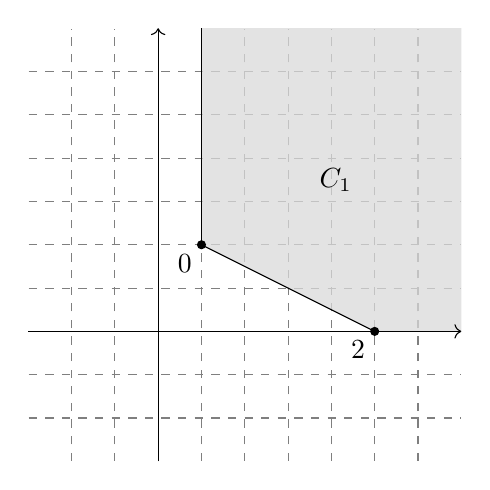
\begin{tikzpicture}[scale=0.55]
\draw (-2.99,-2.99)[dashed, opacity=0.5] grid (6.99,6.99);
\fill[fill=gray!30, opacity=0.75] (1,7)--(1,2)--(5,0)--(7,0)--(7,7);
\draw[->] (-3,0) -- (7,0);
\draw [->] (0,-3) -- (0,7);
\draw (1,7) -- (1,2);
\draw (1,2)--(5,0);
\draw (5,0)--(7,0);
\draw (3.5,3.5) node[right] {$C_1$};
\draw (5,0) node[below left] {2};
\draw (1,2) node[below left] {0};
\fill (5,0) circle[radius=3pt];
\fill (1,2) circle[radius=3pt];
\end{tikzpicture}
\end{minipage} \hspace{4.5cm}
\begin{minipage}{.2\textwidth}
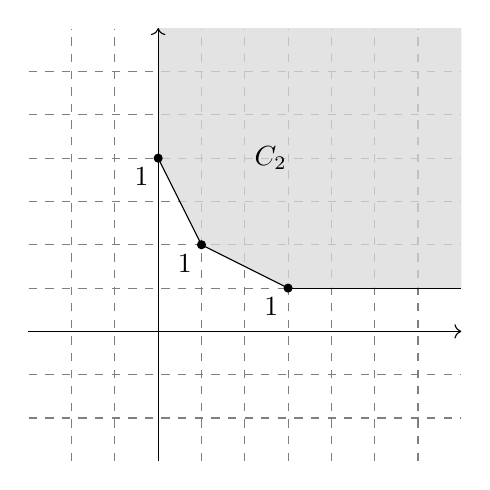
\begin{tikzpicture}[scale=0.55]
\draw (-2.99,-2.99)[dashed, opacity=0.5] grid (6.99,6.99);
\fill[fill=gray!30, opacity=0.75] (0,7)--(0,4)--(1,2)--(1,2)--(3,1)--(7,1)--(7,7);
\draw[->] (-3,0) -- (7,0);
\draw [->] (0,-3) -- (0,7);
\draw (0,7) -- (0,4);
\draw (0,4) -- (1,2);
\draw (3,1)--(1,2);
\draw (3,1)--(7,1);
\draw (2,4) node[right] {$C_2$};
\draw (0,4) node[below left] {1};
\draw (1,2) node[below left] {1};
\draw (3,1) node[below left] {1};
\fill (0,4) circle[radius=3pt];
\fill (1,2) circle[radius=3pt];
\fill (3,1) circle[radius=3pt];
\end{tikzpicture}
\end{minipage}
\end{center}
Their sum and product are respectively:
\[
C_1 \oplus C_2 = (((0,4);1) ,((1,2);0), ((5,0);0) ))
\]
\[
C_1 \odot C_2 = ( ((1,6);1),((2,4);1), ((8,1);3) ))
\]
and are represented below:
\begin{center}
\hspace{-2.5cm}
\begin{minipage}{.2\textwidth}
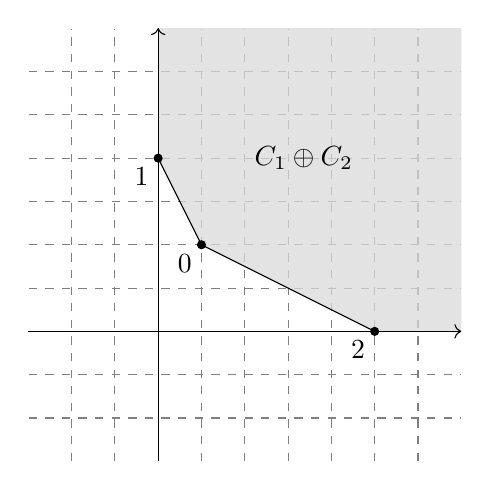
\begin{tikzpicture}[scale=0.55]
\draw (-2.99,-2.99)[dashed, opacity=0.5] grid (6.99,6.99);
\fill[fill=gray!30, opacity=0.75] (0,7)--(0,4)--(1,2)--(5,0)--(7,0)--(7,7);
\draw[->] (-3,0) -- (7,0);
\draw [->] (0,-3) -- (0,7);
\draw (0,7) -- (0,4);
\draw (0,4)--(1,2);
\draw (1,2)--(5,0);
\draw (2,4) node[right] {$C_1 \oplus C_2$};
\draw (0,4) node[below left] {1};
\draw (1,2) node[below left] {0};
\draw (5,0) node[below left] {2};
\fill (0,4) circle[radius=3pt];
\fill (1,2) circle[radius=3pt];
\fill (5,0) circle[radius=3pt];
\end{tikzpicture}
\end{minipage} \hspace{4.5cm}
\begin{minipage}{.2\textwidth}
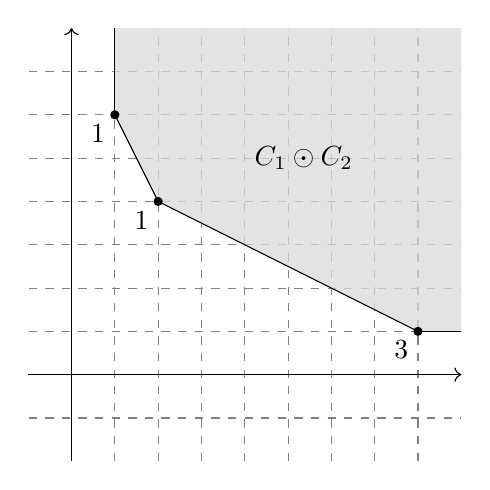
\begin{tikzpicture}[scale=0.55]
\draw (-2.99,-2.99)[dashed, opacity=0.5] grid (6.99,6.99);
\fill[fill=gray!30, opacity=0.75] (-1,7)--(-1,5)--(0,3)--(4,1)--(6,0)--(7,0)--(7,7);
\draw[->] (-3,-1) -- (7,-1);
\draw [->] (-2,-3) -- (-2,7);
\draw (-1,7) -- (-1,5);
\draw (0,3) -- (-1,5);
\draw (0,3)--(4,1);
\draw (4,1)--(6,0);
\draw (7,0)--(6,0);
\draw (2,4) node[right] {$C_1\odot C_2$};
\draw (-1,5) node[below left] {1};
\draw (0,3) node[below left] {1};
\draw (6,0) node[below left] {3};
\fill (-1,5) circle[radius=3pt];
\fill (0,3) circle[radius=3pt];
\fill (6,0) circle[radius=3pt];
\end{tikzpicture}
\end{minipage}
\end{center}
\end{ex}
We adopt the following generalised definition of valuation, as introduced in \cite{eqtrop} and used in \cite{gianmereta}: a \emph{valuation} on a ring $R$ is an idempotent semiring $S$ and a map $v\co R \to S$ satisfying
\begin{enumerate}
\item	$v(0)  = 0_S$,
\item	$v(1) = v(-1) = 1_S$,
\item	$v(ab) = v(a) \odot v(b)$,
\item	$v(a+b) \oplus v(a) \oplus v(b)$ tropically vanishes (i.e. $v(a+b) \preceq v(a) \oplus v(b)$).
\end{enumerate}
Often we will refer to the datum $(R,v)$ of a ring with a valuation as a \emph{valued ring}. 
Notice that a rank 1 valuation $v \co R \rightarrow \T$ can be extended to a rank 2 valuation on the ring $R\{\!\{t\}\!\}$ of Puiseux series (or the subrings of formal Laurent series, power series or polynomials) by the formula
\begin{equation}\label{eq:rank2valuation}
	a_0 t^{n_0} + \cdots \mapsto (n_0, v(a_0)) \in \mathbb{T}_2.
\end{equation}

In order to introduce the main examples of valuations we will be working further on, we need the following definition and lemma. 
\begin{defin}
    Let $\tau$ be a cone as above, and $S$ an idempotent semiring, let
    \[
    S[\![\tau]\!] = \left \{ A = \sum_{\jj \in  \Z^m} s_\jj t^\jj \mid \supp(A) \subseteq  \tau  \right \}.
    \]
    This set, equipped with usual sum and product is the idempotent semiring of multivariate power series supported in $\tau$. When $S$ is a field, this was introduced (with fractional coefficients) for example in \cite{arocacanojung, arocarond}. 
    When $\tau = (\R_{\ge 0})^m$, we will denote $S[\![\tau]\!]$ as $S[\![t_1, \dots t_m]\!]$.
\end{defin}
Notice that restricting the support of a power series to a cone is necessary to make the usual product of power series a well defined operation.
\begin{lem}\label{lem:finite-vertices}
    Let $\tau \subset \R^m$ be a cone and $Z \subset \tau \cap \Z^m$ then $\textup{Vert}_\tau(Z)$ is finite.
\end{lem}
\begin{proof}
    For an element $z \in Z$ we say that $z$ is a \emph{semivertex} if $(Z \setminus \{z\})+ \tau \subsetneq Z + \tau$. Clearly every element in $\textup{Vert}_\tau(Z)$ is a semivertex. Find nonzero (without loss of generality, rational) vectors $v_1, \dots , v_m \in \R^m$ such that $\tau$ can be written as $\{x \in \R^m \mid \langle v_i, x \rangle \ge 0 \text{ for each } i \in [m]\}$. Then for all $z \in \R^m$,
    \[
        z + \tau =\{x \mid x-z \in \tau\} = \{x \mid \langle v_i, x \rangle \ge \langle v_i, z \rangle \text{ for each } i \in [m]\}.
    \]
    For $i \in [m]$, let $\alpha_i = \min_{z \in Z}\langle v_i, z\rangle \ge 0$. This minima exist since $\tau$ is rational, so the normal vectors $v_i$ are rational and after scaling them, we can assume that they are integral. Every lattice point $x \in \tau$ has $\langle x,v_i \rangle \ge 0$, and since both $x$ and $v_i$ are integral, so is their inner product. As a decreasing sequence of non negative integers stabilizes, the minimum exists. 

    Let $D :=\{x \in \R^m \mid \langle x, v_i\rangle \ge \alpha_i \text{ for each } i \in [m]\}$, it is a polyhedron with recession cone $\tau$. By construction we have $\tau \supseteq D \supseteq Z + \tau$, and the convexity of $D$ implies $D \supseteq C_\tau(Z)$. For $i \in [m]$, let $z_i$ such that $\langle z_i , v_i \rangle = \alpha_i$ and $\beta_j := \max_{i \in [m]}\langle v_j, z_i\rangle$.
    Let $E := \{x \in \R^m \mid \alpha_i \le \langle x, v_i\rangle \le \beta_i \text { for each } i \in [m]\}$. This is a bounded subset of $D$. 
    
    We prove the statement by showing that every semivertex is contained in $E$. Note that if $x \in \cup_{j \in [m]} (z_j + \tau)$ and $x \neq z_j$ for all $j$, then $x$ is not a semivertex. Hence, semivertices are contained in the set
    \[
        \left ( D \setminus \bigcup_{j=1}^m (z_j + \tau) \right ) \cup \{z_1, \dots , z_m\}.
    \]
    We now show that the set above is contained in $E$:
    \begin{align*}
        D \supseteq E \cup \bigcup_{j=1} ^m (z_j + \tau) & = E \cup \bigcup_{j=1}^m\{x \in \R^m \mid \langle v_i , x \rangle \ge \langle v_i, z_j \rangle \text{ for all } i \in [m]\} = \\
        & =
        E \cup \{x \in \R^m \mid \exists j \in [m] \text{ s.t. } \langle v_i , x \rangle \ge \langle v_i, z_j \rangle \text{ for all } i \in [m]\} \supseteq 
        \\
        &  \supseteq 
        E \cup \{x \in \R^m \mid \langle v_i , x \rangle \ge \beta_i \text{ for all } i \in [m]\} =
        \\
        & = D.
    \end{align*}
    So we get
    \[
        E \supseteq \overline{ \left (D \setminus \bigcup_{j=1}^m (z_j + \tau) \right ) } \supseteq \left ( D \setminus \bigcup_{j=1}^m (z_i + \tau) \right ) \cup \{z_1, \dots , z_m\}.
    \]
    Thus all the semivertices lie in $E$. This implies that $\textup{Vert}_\tau(Z) \subseteq E$ and since $E$ is bounded, $\textup{Vert}_\tau(Z)$ is finite.
\end{proof}
\begin{oss}
    The Lemma above holds with analogous proof also allowing fractional exponents, since the definition of fractional Laurent series, as it can be found in \cite{arocacanojung}, implies the existence of a least common multiple of the denominators of the exponents appearing in each series.
\end{oss}
\begin{oss} \label{oss:conv-as-quotient}
 Given a cone $\tau$ and an idempotent semiring $S$, it follows from Lemma \ref{lem:finite-vertices} that the idempotent semiring $\textup{Conv}(\tau,S)$ of Definition \ref{def:conv-boolean-semirings} can be realised as the quotient of $S[\![\tau]\!]$ by the semiring congruence
\begin{center}
\begin{tabular}{ c c c }
 & & $C_\tau(\supp(A)) = C_\tau(\supp(B)) $ \\ 
 $A = \sum a_\jj t^\jj  \sim  B =\sum b_\jj t^\jj $ & $\iff$ & and \\  
 &  & $a_\jj = b_\jj \text{ for all } \jj \in \textup{Vert}_\tau(\supp(A))$   
\end{tabular}
\end{center}
Also, given $A \in \pkcone \tau$, we have that the convex hull of the support of $A$ with respect to $\tau$ has finitely many vertices. This allow us to define the following valuations:
\end{oss}
\begin{ex}\label{ex:conv-vals}
\begin{enumerate}
    \item Given a cone $\tau \subset \R^m$ and a field $K$, the map 
            \[
	           w_\tau \co  \pkcone \tau  \to \textup{Conv}(\tau,\B)
		\]
    sending an element $A \in \pkcone \tau $ to the convex hull of its support is a valuation. As noted in Remark \ref{oss:Conv-m=1}, when $m=1$, $\textup{Conv}_1(\B) \subset \T$ and it is easy to check that the valuation $w$ becomes the $t$-adic valuation $\pk \rightarrow \T$ sending a univariate power series to its leading order.
    \item  Given a cone $\tau \subset \R^m$, let $v_K \co K \rightarrow \T$ be a valued field. With a similar procedure to that illustrated in \ref{eq:rank2valuation}, we build a refined version of the valuation $w$ above. The map
	\[ 
		v_\tau \co \pkcone \tau \to \textup{Conv}(\tau,\T)
	\] 
    given by sending $A \in \pkcone \tau$ to the convex hull of its support with respect to $\tau$, with vertices weighted by the valuation $v_K(a_{\mathbf{n}})$ of the coefficients of the corresponding terms, is a valuation.
    Analogously as for the valuation $w$ of point (1), for $m=1$, $\textup{Conv}_1(\T) \subset \T_2$ and we retrieve the valuation $\pk \rightarrow \T_2$ obtained by refining the $t$-adic valuation as illustrated in \ref{eq:rank2valuation}. 
\end{enumerate}

\end{ex}
\begin{oss}
    Notice that the valuation $v_\tau$  of point (2) above can be defined analogously for every valued ring $R \rightarrow S$, to be a valuation $R[\![\tau]\!] \rightarrow \textup{Conv}(\tau, S)$. As here we focus on the case were $R$ is a tropically valued field, we will just look at the case of Example \ref{ex:conv-vals} above.
\end{oss}
\begin{oss}
    For every cone $\tau$, the valuation $w_\tau$ above is a surjective valuation. On the other hand, $v_\tau$ is surjective if $v_K$ is a surjective valuation (or if we restrict the weights to take values in the value group of $v_K$). Furthermore, notice that for a valued field $v_K \co K \rightarrow \T$ the valuations $w$ and $v$ fit in the following commutative diagram with the map $\sigma_0$ of Remark \ref{oss:Conv-m=1}, for every $\tau$:
    \[
        \begin{tikzcd}
            & \pkcone \tau  \arrow[dr, "w_\tau"] \arrow[dl, swap, "v_\tau"]&  \\
             \textup{Conv}(\tau,\T) \arrow[rr, "\sigma_0"]  & & \textup{Conv}(\tau, \B) .
        \end{tikzcd}
    \]
\end{oss}

We introduce here another semiring and a valuation that will turn out to be useful in Section \ref{section:grobner}: 
\begin{defin} \label{def:lead-semiring}
Let $\omega \in \R^m$ with rationally independent coordinates, then the following
    \[
        v_1 \preceq_\omega v_2 \iff \langle v_1 , \omega \rangle \le \langle v_2, \omega \rangle,
    \]
is a total order on $\Q^m$. 
Given an idempotent semiring $S$, let $\textup{Lead}_\omega(\Q^m,S)$ be the semiring obtained by endowing $(\Q^m \times (S \setminus\{0_S\} ) ) \cup \{\infty\}$ with the following semiring structure: 
    \[
        (\jj_1, s_1) \oplus (\jj_2, s_2) := \begin{cases}
        \left ( \jj_1, s_1  \right ) & \text{if } \jj_1 = \min_{\preceq_\omega} \{\jj_1, \jj_2\} 
        \\
        \left ( \jj_2, s_2  \right ) & \text{if } \jj_2 = \min_{\preceq_\omega} \{\jj_1, \jj_2\} 
        \\
        \left ( \jj, s_1 \oplus_S s_2  \right ) & \text{if } \jj := \jj_1 = \jj_2 
        \end{cases}
    \]
    
    \[
        (\jj_1, s_1) \odot (\jj_2, s_2) := \left ( \jj_1 + \jj_2, s_1 \odot_S s_2 \right ).
    \]
Its additive identity is $\infty$ and its multiplicative identity is $(0_{\Q^m}, 1_S)$. This semiring is an $S$-algebra by viewing $S$ as the subsemiring $\{(0_{\Q^m}, s) \mid s \in S\} \subset \textup{Lead}_\omega(\Q^m,S)$. 

Furthermore, we will denote as $\textup{Lead}_\omega(G,S)$ the semiring obtained analogously, considering any additive submonoid $G$ of $\Q^m$.
\end{defin}
\begin{oss}
    In case the canonical partial order $\preceq_S$ of $S$ is a total order, e.g.\ for $S=\T$ or any of its subsemirings, the sum of the semiring $\textup{Lead}_\omega(\Q^m,S)$ above accounts to taking the minimum with respect to the lexicographic order induced by $\preceq_\omega$ and $\preceq_S$.
\end{oss}
\begin{ex} \label{ex:omega-val-tau}
Given $\omega \in \R^m$ with rationally independent coordinates, let $H_\omega$ be the halfspace $\{x \in \R^m \mid \langle x, \omega \rangle \ge 0 \}$. Given a cone $\tau \subset H_\omega$, the vector $\omega$ induces the total  order $\preceq_\omega$ on $\tau \cap \Z^m$ as above.
Given a valued field $v_K \co K \rightarrow \T$, then the map 
    \[
        v_{\tau,\omega} \co \pkcone \tau \rightarrow \textup{Lead}_\omega(\tau \cap \Z^m,\T)
    \]
    defined as:
    \[
        A=\sum_{\jj \in \tau \cap \Z^m} a_\jj t^\jj \mapsto (\overline \jj, v_K (a_{\overline \jj})),
    \]
    where $\overline \jj= \min_{\preceq_\omega} \supp(A)$, is a valuation. When $m=1$, this is again the valuation $\pk \rightarrow \T_2$ refining the $t$-adic valuation as in \ref{eq:rank2valuation}.
\end{ex}
\subsection*{Differential semirings}
Given an idempotent semiring $S$, an
additive map $d\co S \to S$ is said to be a \emph{tropical differential} if it satisfies the tropical Leibniz relations:  for any two elements  $x,y \in S$ the expression
\[
d(xy) \oplus xd(y) \oplus yd(x)
\]
tropically vanishes. Note that we can view the tropical Leibniz relations as the tropicalization of the usual Leibniz relations. Furthermore, as $S$ is an idempotent semiring, if $d\co S \to S$ satisfies the usual Leibniz rule, it is a tropical differential. In this case we will say that $d$ is a \emph{strict} tropical differential.


\begin{defin}
A \emph{partial differential idempotent semiring} $(S, \{ d_{S,i}\}_{i \in [m]} \})$ with $m$ commuting differentials is an idempotent semiring $S$ equipped with $m$ pairwise commuting tropical differentials $d_{S,i} \co S \rightarrow S$. Analogously as for rings, a homomorphism of differential semiring is a homomorphism of semirings commuting with the differentials.

We will often drop the adjectives \emph{partial} and \emph{idempotent} in the following.
\end{defin}


The two main examples of differential semiring we will work with are the following:
\begin{ex}\label{ex:diffsemirings}
\begin{enumerate}
\item Consider the idempotent semiring $\pbb m$ of multivariate formal power series with boolean coefficients. Endowing it with the differentials $\{d/dt_i\}_{i \in [m]}$ defined by
\[
\frac{d}{dt_i}(t_j^n) = \begin{cases} 
t_i^{n-1} & n \geq 1, i=j\\
\infty & \text{otherwise}
\end{cases}
\]
and extended by Leibniz rule we obtain a strict partial differential semiring. 
\item Consider the idempotent semiring of multivariate tropical power series $\ptt m$. Given a nontrivial valuation $v\co \mathbb{N} \to \mathbb{T}$, let $(d/dt_i)_v$ be defined as 
\[
\left (\frac{d}{dt_i} \right)_v(t_j^n) = \begin{cases} 
v(n)t_i^{n-1} & n \geq 1, i=j\\
\infty & \text{otherwise},
\end{cases}
\]
then $(d/dt_i)_v$ is a tropical differential for every $i$ and we will denote as $\ptt {m}_v$ the (non-strict) differential semiring $(\ptt m, \{(d/dt_i)_v\}_{i \in [m]})$.
\end{enumerate}
\end{ex}

 Analogously to what is proven in \cite[Proposition 3.2.3]{gianmereta}, for any $m$, given a non-strict differential semiring $(S, \{d_{S,i}\}_{i \in [m]})$, there is no family of tropical differentials $\{d_i\}$ on $\basic S n$ extending the $d_{S,i}$'s such that $(\basic S n, \{d_i\}_{i \in [m]})$ is the free differential algebra over $S$ on $n$ generators. The definition of the differential semiring 
 \[
 (\diff S n , \{d_i\}_{i \in [m]})
 \]
 of differential polynomials over $(S,\{d_{S,i}\}_{i \in [m]})$ is quite convoluted and we are not going to recall it here, but  all the details can be found in \cite[Section 3.4]{gianmereta} and \cite[Chapter 8]{tesimereta}. Furthermore, $\diff S n$ satisfies the desirable universal property, i.e.\ given a differential algebra $S'$ over $S$, the following bijection holds: 
\[
	\mathrm{Hom}_{S\textup{-Alg}}(S\{x_1, \ldots, x_n\}, S') \cong (S')^n.
\]
It is important to notice that the construction of \cite{gianmereta,tesimereta} gives back Ritt's construction as in \ref{eq:ritt-polynomials} when the $d_{S,i}$'s are strict differentials, so in particular when $S$ is a differential ring or $\pbb m$. In general there is only an inclusion of algebras over $S$:
\[
    \basic S n \subseteq \diff S n .
\]
\subsection*{Tropical pairs}
The central objects in the theory of TDEs are the so-called tropical pairs, playing in this theory an analogous role to that of rings and algebras in the theory of polynomial equations: 
\begin{defin}
A \emph{(partial) tropical pair} $\mathbf{S}$ with $m$ differentials is a homomorphism of idempotent semirings $\pi\co (S_1,\{d_{S_1,i}\}_{i \in [m]}) \to S_0$, where $(S_1,\{d_{S_1,i}\}_{i \in [m]})$ is a partial differential semiring with $m$ commuting differentials. We will say that $\mathbf S$ is strict if $S_1$ is a strict differential semiring. A morphism of pairs $\sigma$ from $(S_1\to S_0)$ to $(T_1
\to T_0)$ is a commutative diagram of idempotent semirings
\[
\begin{tikzcd}
S_1 \arrow[d] \arrow[r, "\sigma_1"] & T_1 \arrow[d] \\
S_0 \arrow[r, swap, "\sigma_0"]           & T_0          
\end{tikzcd}
\]
in which the upper horizontal arrow $\sigma_1$ is a morphism of partial differential idempotent semirings.
\end{defin}
These maps can be thought of as sending elements of $S_1$ to their leading orders. This will actually be the case for the instances considered in the following of this work. We introduce them in the following example:

\begin{ex}\label{ex:pairs}
\begin{enumerate}
    \item Consider $(\pb, d)$ as in point (1) of Example \ref{ex:diffsemirings} with $m=1$. The homomorphism $\Psi \co \pb \to \mathbb{T}$ defined by $t^n \mapsto n$ is a tropical pair.
    \item Consider $ \Phi\co \pt_v\to \mathbb{T}_2$, where the source has any of the differentials from point (2) of Example \ref{ex:diffsemirings} and the morphism $\Phi$ is given by
    \[
        (a_{n_0} t^{n_0} + a_{n_1} t^{n_1} + \cdots) \mapsto (n_0, a_{n_0}).
    \] 
    It is a tropical pair.
    \item For every $m$, let $(\pbb m, \{d / d t_i\}_{i \in [m]})$ as in Example \ref{ex:diffsemirings} and consider the partial tropical pair
            \[
	           \Psi_m \co  \pbb m \to \textup{Conv}_m(\B).
		\]
    sending an element $B \in \pbb r$ to the convex hull of its support. For $m=1$, analogously to point (1) of Example \ref{ex:conv-vals}, $\Psi_1$ is the pair $\Psi$ of point (1). We will denote this pair by $\mathbf T _m$
    \item Consider the partial tropical pair
		\[ 
		\Phi_m \co {\ptt m}_v \to \textup{Conv}_m(\T),
		\] 
    where the source has differentials as in Example \ref{ex:diffsemirings} for a valuation $v$. The morphism $\Phi_m$ is given by sending $B \in {\ptt m}_v$ to the convex hull of its support with vertices weighted by the coefficients of the corresponding leading terms.
    When $m=1$, $\Phi_1$ is the pair $\Phi$ of point (2). We will denote this pair as $\mathbf S _m$.
    \item Fix $m$ and let $v$ be a valuation as in Example \ref{ex:diffsemirings}. Given a monomial ordering $t_{l_1} \preceq t_{l_2} \preceq \dots \preceq t_{l_m} $ of the variables of ${\ptt m}_v$, let  
    \[
    \Upsilon_m \co {\ptt m}_v \rightarrow \T_{m+1}
    \]
    be the map sending a multivariate power series $ A:=\sum_{\jj \in \N^m} a_\jj t^\jj$ to $(\overline \jj, a_{\overline \jj})$ where $\overline \jj = \min_\preceq 
    \supp (A)$.
    When $m=1$ the pair $\Upsilon_1$ recovers $\Phi$ of point (2), and the analogous map defined over $\pbb m$ recovers the pair $\Psi$ of point (1) for $m=1$.  
	\end{enumerate}
\end{ex}
\begin{defin}
A pair $\pi\co (S_1,\{d_{S_1,i}\}_{i \in [m]}) \to S_0$ is said to be \emph{reduced} if there is no nontrivial congruence closed with respect to the action of $\{d_{S_1, i}\}_{i \in [m]}$ and contained in the semiring congruence $\ker(\pi) = \{(a ,b) \mid \pi(a)=\pi(b)\}$. Reduced pairs form a subcategory of the category of pairs and it is possible to associate to each pair a reduced pair, its \emph{reduction}, in a functorial way (\cite[4.3]{gianmereta}).
\end{defin}
All the pairs of Example \ref{ex:pairs} are reduced (see \cite[Chapter 6]{tesimereta} for the details). Since all the pairs we will work with in our treatement are reduced, from now on every instance of the word ``pair'' has to be intended as ``\emph{reduced} pair''. 

Given a pair $\mathbf{S}$, the category of $\mathbf{S}$-algebras is the category of pairs $\mathbf{T}$ under $\mathbf{S}$. A typical example of an $\mathbf S$-algebra is $\diff {\mathbf S} n$, the algebra of differential polynomials in $n$ variables over $\mathbf S$. It satisfies a universal property similar to that of Ritt's polynomials, see \cite[Proposition 4.1.4]{gianmereta}. 
\begin{defin} \label{def:diff-poly-over-pair}
We denote by $(S_0 | S_1)\{x_1, \ldots, x_n\}$ the pushout of the following diagram: 
\begin{equation}\label{eq:pushout-diagram}
\begin{tikzcd}
    S_1 \arrow[r] \arrow[d] & S_1\{x_1, \ldots, x_n\} \\
    S_0  & .
\end{tikzcd}
\end{equation}
The pair $\diff {\mathbf{S}} n$ is the reduction of the pair
    \[
        \diff {S_1}n \rightarrow (S_0 | S_1)\{x_1, \ldots, x_n\}.
    \]
\end{defin}
As for the definition of $\diff S n$, we will not get in the detail of a concrete  realisation of the $S_0$-algebra $(S_0 | S_1)\{x_1, \ldots, x_n\}$: for our scope, it is enough to say that we have the following inclusion of $S_0$-algebras:
\[
    \basic {S_0} {n} \subseteq (S_0 | S_1)\{x_1, \ldots, x_n\}.
\]
which is an equality if and only if $S_1$ is a strict differential semiring.

\subsection*{TDEs, differential enhancements and tropicalization}
We can finally state formally the definition of tropical differential equation that we will use, and how solutions to such an equation look like:
\begin{defin}\label{defin:tropical-solutions}
    A tropical differential equation over the pair $\mathbf S = (S_1 \stackrel{\Phi}{\to} S_0)$ is an element of $f \in \basic {S_0} {n}$. A solution to $f$ in an $\mathbf S$-algebra $\mathbf T = (T_1 \stackrel{\Psi}{\to} T_0)$ is an element $(y_1, \dots , y_n) \in T_1^n$ such that by plugging in $\Psi(d^{\mathbf j} (y_i))$ for $x_i^{(\mathbf{j})}$ in $f$ the result tropically vanishes. We will denote by $\textup{Sol}_{\mathbf T}(E)$ the set of solutions to a system $E$ in $\mathbf T$.
\end{defin}
As stated in \cite[Proposition 4.5.1]{gianmereta} or \cite[Theorem 6.3.5 and Theorem 8.3.5]{tesimereta}, the functor of solutions to a tropical differential equation can be corepresented by a specific quotient of the pair of differential polynomials over $\mathbf S$ by a bend congruence (see \cite{eqtrop} for a definition).

Lastly, we describe how to tropicalize a system of PDEs with coefficients in a valued ring $v \co R \rightarrow S$ to obtain the associated system of TDEs, and how to tropicalize its solutions. For systems of polynomial equations this is done via the valuation $v$, while here we need the more refined datum of a differential enhancement of a valuation. 

\begin{defin}
    Let $R$ be a ring and $S$ be an idempotent semiring. We say that a map $ \widetilde v \co R \rightarrow S$ is a \emph{submultiplicative seminorm} if:
    \begin{enumerate}
        \item $\widetilde v(0_R) = 0_S$ and $\widetilde v(1_R) = 1_S$;
        \item $\widetilde v(a+b) \preceq \widetilde v(a) \oplus \widetilde v(b)$;
        \item $\widetilde v(ab) \preceq \widetilde v(a) \odot \widetilde v(b)$.
    \end{enumerate}
\end{defin}

\begin{defin}\label{def:diff-enhan}
For any $m$, given a partial differential ring $(R, \{d_{R,i}\}_{i \in [m]})$ and a valuation $ v\co R \to S_0$ to an idempotent semiring $S_0$, a \emph{differential enhancement of $v$} is a partial reduced pair $\mathbf{S} = (S_1\to S_0)$ with $m$ differentials and a submultiplicative seminorm $\widetilde{v}\co R \to S_1$ such that:
\begin{enumerate}
\item for all $x\in R$, for all $i \in [m]$, $d_{S_1,i} \widetilde{v}(x) = \widetilde{v}(d_{R,i} x)$;
\item the following diagram commutes:
\begin{center}
\begin{tikzcd}
& S_1 \arrow[d]  \\
R \arrow[ur, "\widetilde{v}"] \arrow[r, swap, "v"] & S_0 .
\end{tikzcd}
\end{center}
\end{enumerate}

We will use the term \emph{differentially enhanced valuation} $\mathbf{v}=(v,\widetilde{v})\co R \to \mathbf{S}$ to mean a seminorm $v$ together with a differential enhancement $\widetilde{v}$. 
\end{defin}

\begin{oss}
With analogous proof as that of \cite[Proposition 4.7.4]{gianmereta}, one can prove that for every $m$ the submultiplicative seminorm $\widetilde v$ restricts to a valuation on the subring of constants of the ring $R$, i.e.\ the subring
\[
    \{x \in R \mid d_{R,i}x = 0_R \text{ for all $i \in [m]$}\}.
\]
\end{oss}
Thanks to the pair $\mathbf S$ being reduced, the differential enhancement is unique.
\begin{lem} \label{lem:Diff-Berk-To-Berk}
Given a valued partial differential ring with $m$ differentials $v: R \rightarrow S_0$, fix a reduced pair $\mathbf{S}: S_1 \xrightarrow{\pi} S_0$ and let $\widetilde v$ and $\widetilde v '$ be two maps $R \rightarrow S_1$ such that both $(\mathbf {S}, \widetilde v)$ and $(\mathbf{S}, \widetilde v ')$ are differential enhancements of $v$. Then $\widetilde v = \widetilde v '$.
\end{lem}   
\begin{proof}
Let $a \in R$, as both $(\mathbf {S}, \widetilde v)$ and $(\mathbf{S}, \widetilde v ')$ are differential enhancements of $v$, we have $\pi (\widetilde v (a)) = v(a) = \pi(\widetilde v ' (a))$, thus $(\widetilde v (a), \widetilde v '(a)) \in \ke \pi$. Furthermore, for the same reason and since $\widetilde v$ and $\widetilde v '$ commute with the differentials, we have $ (d^\jj (\widetilde v (a)), d^\jj ( \widetilde v '(a))) \in \ke \pi$ for every $\jj \in \N^m$. As $\pi$ is a reduced pair, this implies $d^\jj (\widetilde v (a)) = d^\jj ( \widetilde v '(a))$ for every $n$. So in particular $\widetilde v (a) = \widetilde v '(a)$. Hence $\widetilde v = \widetilde v '$.
\end{proof}
\begin{oss}
If $\mathbf{S}$ is not reduced Lemma \ref{lem:Diff-Berk-To-Berk} does not hold. Indeed, consider the non-reduced pair $\pt_{v_{\text{triv}}} \xrightarrow{\pi} \T$, sending a tropical power series to its leading exponent. Then for a field $K$, let $R = (K[\![s]\!])[\![t]\!]$ equipped with the $d/dt$ differential and let $v_t$ (resp. $v_s$) the $t$-adic (resp. $s$-adic) valuation on $R$ and $\nu : K[\![s]\!] \rightarrow \B$ the trivial valuation. It is possible to complete the following diagram:
		\[
		\begin{tikzcd}
		& \pt_{v_{\text{triv}}} \arrow[d, "\pi"] \\
		R \arrow[r, "v_t"] & \T 
		\end{tikzcd}
		\] 
to a commutative diagram with a map $R \rightarrow \pt_{v_{\text{triv}}}$ in two different ways by the two maps given by coefficientwise application of $\nu$ and $v_s$.
\end{oss}
We introduce here several examples of differential enhancements that we will use in the following.
\begin{ex}\label{ex:diff-enhancements}
\begin{enumerate}
\item Let $v_{\text{triv}} \co K \rightarrow \B$ be a trivially valued field. As seen in point (1) of Example \ref{ex:conv-vals}, the valuation obtained by extending the trivial valuation as in \ref{eq:rank2valuation} is the $t$-adic valuation $w \co \pk \to \T$. It admits a differential enhancement on the pair $\mathbf T _1$ of point (1) of Example \ref{ex:pairs}:
\begin{center}
\begin{tikzcd}
& \pb \arrow[d] \\
\pk \arrow[ur, "\widetilde{w}"] \arrow[r, swap, "w"] & \mathbb{T} 
\end{tikzcd}
\end{center}
in which the map $\widetilde w$ sends a power series over $K$ to its coefficientwise trivial valuation.  This is the differentially enhanced valuation used by Grigoriev \cite{grig} in his framework and subsequent works
\cite{aroca,FT20} for ODEs.
\item Let $v_K \co K \rightarrow \T$ be a nontrivially valued field and let $v \co \pk \rightarrow \T_2$ the extension of $v_K$ to $\pk$ as in \ref{eq:rank2valuation}. The valuation $v$ admits a differential enhancement
\begin{center}
\begin{tikzcd}
& \pt_{v_K} \arrow[d] \\
\pk \arrow[ur, "\widetilde{v}"] \arrow[r, swap, "v"] & \mathbb{T}_2 
\end{tikzcd}
\end{center}
to the pair $\mathbf S _1$ of point (2) of Example \ref{ex:pairs}. Analogously as above, the map $\widetilde v$ is defined by coefficientwise application of $v_K$.
\item Given a trivially valued field $K$, the valuation $v \co \pkk r \to \textup{Conv}_m(\B)$ sending a power series to the convex hull of its support, introduced in point (1) of Example \ref{ex:conv-vals}, admits a differential enhancement to the pair $\mathbf T _m$ of point (3) of Example \ref{ex:pairs}:
	\begin{center}
		\begin{tikzcd}
		&\pbb m \arrow[d, "\Psi_m"] \\
		\pkk m \arrow[ur, "\widetilde{w}"] \arrow[r,swap, "w"] &  \textup{Conv}_m(\B)
		\end{tikzcd}
	\end{center}
where $\widetilde w$ is the map $\pkk r \to \pbb r$ given by coefficientwise trivial valuation, i.e. taking the support. This is the differentially enhanced valuation used in \cite{sebastian,  cotterill, sebastianmereta} in the context of PDEs. This recovers the differential enhancement of point (1) for $m=1$. We will denote the differentially enhanced valuation $(w, \widetilde w)$ as $\mathbf w$.
\item Given a valued field $v_K \co K \rightarrow \T$, consider the valuation $v \co \pkk r \to \textup{Conv}_m(\T)$, as defined in point (2) of Example \ref{ex:conv-vals}. This admits a differential enhancement to the pair $\mathbf S _m$ of Example \ref{ex:pairs} part (4):
	\begin{center}
		\begin{tikzcd}
		& \ptt m _{v_K} \arrow[d, "\Phi_m"] \\
		\pkk  m \arrow[ur, "\widetilde{v}"] \arrow[r,swap,"v"] & \textup{Conv}_m(\T) 
		\end{tikzcd}
	\end{center}
	where $\widetilde v$ is given by coefficientwise application of $v_K$. This recovers the differential enhancement of point (2) for $m=1$. We will denote the differentially enhanced valuation $(v, \widetilde v)$ as $\mathbf v $.
\end{enumerate}
\end{ex}
For any $m$, the differential enhancement of point (4) (and that of point (2)) of the example above, allows us to keep track of the valuation of the coefficients of a power series in $\pkk m$. Notice that there is a morphism $\sigma = (\sigma_0,\sigma_1)$ of reduced pairs between $\mathbf T _m$ and $\mathbf S _m$ of Example \ref{ex:pairs}:
\begin{equation} \label{diagram:refined-to-grig}
		\begin{tikzcd}
		\ptt m _{v_K}  \arrow[d] \arrow[r, "\sigma_1"] & \pbb m \arrow[d]\\
		 \textup{Conv}_m(\T) \arrow[r, "\sigma_0"] &  \textup{Conv}_m(\B)
		\end{tikzcd}
\end{equation}
where the $\sigma_0$ is the homomorphism discussed in Remark \ref{oss:Conv-m=1} and $\sigma_1$ is defined by sending a tropical multivariate power series to its support. This  makes the pair $\mathbf T _m$ into an $\mathbf S _m$-algebra. 
Furthermore, $\sigma$ sends the differentially enhanced valuation $\mathbf{v}$ to the $\mathbf{w}$ of Example \ref{ex:diff-enhancements}. Thus it is the link between the framework for TDEs as developed by Grigoriev in \cite{grig} and the more general one of \cite{gianmereta}: the new framework refines Grigoriev's one and includes it as a special case, thus solutions for a differential equations in the refined setting are also solutions in Grigoriev's sense. 

\begin{defin}
    Given a totally ordered commutative monoid $(G, +, \preceq)$, let $\widetilde G$ be the idempotent semiring $(G \cup \{\infty\}, \min_{\preceq}, +)$.
\end{defin}
\begin{oss}\label{oss:restr-of-diff-enh}
Let $\Gamma_K$ be the value group of $v_K$. As in the following we will need the differentially enhanced valuation $\mathbf{v}$ to be surjective (i.e. both $v$ and $\widetilde v$ to be surjective), we will consider its restriction to the pair $\mathbf{\Gamma}_m = (\widetilde{\Gamma}_K[\![t_1, \dots , t_m]\!] \stackrel{\Phi_m}{\to} \textup{Conv}_m(\widetilde{\Gamma}_K))$, obtained by restricting the coefficients and the weights to the value group $\Gamma_K$. The tropical pair $\mathbf{\Gamma}_m$ is the quotient map discussed in Remark \ref{oss:conv-as-quotient}. The differentially enhanced valuation $\mathbf{v}: \pkk m \rightarrow \mathbf{\Gamma}_m$ is surjective.
\end{oss}

We are finally ready to define the differential tropicalization of a system of PDEs with coefficients in a differential ring, and of the solutions of this system. Let us fix a partial differential ring $R$ and a differentially enhanced valuation 
\[
    \mathbf v =(v,\widetilde{v})\co (R,\{d_{R,i}\}_{i \in [m]}) \to \mathbf{S}
\]
to a reduced pair $\mathbf S$. With this data:
\begin{enumerate}
\item we tropicalize points $r \in R^n$ via the map $\trop_{\widetilde v}\co R^n \to S_1^n$ defined by applying
$\widetilde{v}$ componentwise.
\item we tropicalize differential equations by applying $v$ coefficientwise to define a map 
\[
\trop_v\co \diff R n \to \basic {S_0} n.
\]
\end{enumerate}

In this context, given a differential ideal $I \subset \diff R n$, the statement of a fundamental theorem is the equality 
\[
	\textup{Sol}_{\mathbf S}(\trop_{v} (I)) = \trop_{\widetilde v}(\textup{Sol}_{R}(I)). 
\]
In case the differentially enhanced valuation considered is $\mathbf w$ of point (3) of Example \ref{ex:diff-enhancements}, i.e. that of Grigoriev's setting, this is the main result of \cite{aroca} for $m=1$, and of \cite{sebastian}, for every $m$. In general, the inclusion $\textup{Sol}_{\mathbf S}(\trop_{v} (I)) \subset \trop_{\tilde v}(\textup{Sol}_{R}(I))$ holds, as proven in \cite[Proposition 5.2.2]{gianmereta} (see also \cite[Proposition 7.1.5]{tesimereta} for a proof of this result in a more general formulation).

The main aim of the present work is to prove a fundamental theorem for the differential enhancement $\mathbf v$ of point (2) of Example \ref{ex:diff-enhancements} and for every $m$, and to develop a Gröbner theory that allows us to extend and incorporate in the present theory the results of \cite{FT20} and \cite{hugao}.

\begin{oss}
    Notice that, using the notation of Example \ref{ex:diff-enhancements} and Diagram \ref{diagram:refined-to-grig},  the following inclusion holds for every $m$:
    \[
           \sigma_1 \left ( \textup{Sol}_{\mathbf S _m}(\trop_{v} (I))  \right)
           \subset 
            \textup{Sol}_{\mathbf T _m}(\trop_{w} (I))  
    \]
    and in general it is strict, as showed in \cite[Example 4.2.2]{gianmereta}. This is evidence that the general framework developed in \cite{gianmereta} and \cite{tesimereta} refines the previous one of Grigoriev.
\end{oss}

\section{Fibres of the tropicalization}\label{section:preliminaries}

The main aim of this section is to prove Corollary \ref{corolla:remark+proposition}, which given a differential ideal $I$ gives a necessary and sufficient condition for points to lie in the tropicalization of the solution set of $I$ in terms of non-emptiness of a certain family of sets, obtained as the zero loci of a family of polynomials. This will be essential to the proof of the Fundamental Theorem. The key step in the proof of this corollary is Proposition \ref{Prop:limit-empty-iff-some-empty}, which is a generalization of \cite[Theorem 1]{bouliermodel}.

On the way, we improve a result of Payne \cite{payne09fibers} on Zariski-density of fibres of tropicalization of algebraic varieties, showing that (provided the ambient field is uncountable) a fibre of the tropicalization of an algebraic variety cannot be covered by countably many constructible sets, unless it is covered by finitely many of them. For the proof we use some basic model theory, so we recall some notions and facts from the area. The interested reader is invited to consult \cite{poizat2011course} for more details. 

\begin{defin}
    Let $\mathcal{L}$ be a first-order language, $A$ a set. An $\mathcal{L}$-\textit{type over} $A$ is a set of $\mathcal{L}_A$-formulas, that is, a set of formulas in the language $\mathcal{L} \cup \{c_a \mid a \in A\}$ where each $c_a$ is a constant symbol not appearing in $\mathcal{L}$.

    A type $p$ is \textit{realized} in a structure $\mathcal{S}$ if there is a tuple $s$ in the universe of $\mathcal{S}$ such that for all $\phi(x) \in p$, $\mathcal{S} \vDash \phi(s)$.
\end{defin}

\begin{defin}
    Let $T$ be complete $\mathcal{L}$-theory, $\kappa$ a cardinal. A model $\mathcal{M} \vDash T$ is $\kappa$-\textit{saturated} if for every subset $A$ of the universe of $\mathcal{M}$ with $|A| < \kappa$ and every type $p$ over $A$, if $p$ is realized in some elementary extension of $\mathcal{M}$ then it is realized in $\mathcal{M}$.

    If $|\mathcal{M}|=\kappa$ and $\mathcal{M}$ is $\kappa$-saturated, then we say $\mathcal{M}$ is \textit{saturated}.
\end{defin}

Recall that for $p=0$ or a prime, $\mathsf{ACF}_p$ denotes the complete theory (in the language of rings) of algebraically closed fields of characteristic $p$. The following is well-known.

\begin{teorema}\label{thm:acf-are-saturated}
    Let $K$ be an uncountable algebraically closed field of characteristic $p$, with $p=0$ or prime. Then $K$ is saturated model of the theory $\mathsf{ACF}_p$.
\end{teorema}

\begin{proof}
    By \cite[Theorem 14.2]{poizat2011course}, if a theory is \textit{$\lambda$-stable} for a cardinal $\kappa$ (see \cite[Section 11]{poizat2011course} for the definition) then it has a saturated model of size $\kappa$. By \cite[Example 13.3.7]{poizat2011course}, for each characteristic $p$ the theory $\mathsf{ACF}_p$ is $\omega$-stable and hence by \cite[Theorem 13.11]{poizat2011course} it is $\kappa$-stable for every $\kappa$.

    By Steinitz's theorem \cite[Theorem VI.1.12]{hungerford1974algebra}, for every fixed characteristic $p$ and uncountable cardinal $\kappa$ there is (up to isomorphism) only one algebraically closed field of characteristic $p$ and size $\kappa$. Saturation is preserved under isomorphism, so this proves the statement.
\end{proof}

\begin{lem}\label{lem:v-notin-xi}
    Let $V$ be an algebraic variety defined over an uncountable algebraically closed field $F$, $\{X_i \mid i \in \mathbb{N}\}$ a set of proper constructible subsets of $V$ defined over $F$, with $\dim X_i < \dim V$ for each $i$.

    Then there is $v \in V(F)$ such that $v \notin X_i$ for each $i \in \mathbb{N}$.
\end{lem}

\begin{proof}
    Let $A \subseteq F$ be a countable subset over which $V$ and all the $X_i$'s are defined. Let $p_0$ be the set of formulas over $A$ in the ring language $p_0:=\{x \in V\} \cup \{x \notin X_i \mid i \in \mathbb{N}\}$. Since $\dim X_i < \dim V$, every finite subset of $p_0$ is consistent, so $p_0$ can be extended to a complete type $p$ over $A$, which by saturation is realized in $F$. 
\end{proof}

\begin{lem}\label{lemma:curve-through-two-points}
    Let $V$ be an algebraic variety defined over an uncountable algebraically closed field $F$, $v_0 \in V(F)$, $\{X_i \mid i \in \mathbb{N} \}$ a set of constructible subsets of $V$ with $\dim X_i <\dim V$.

    There is a curve $C \subseteq V$ such that $v_0 \in C(F)$ and for each $i \in \mathbb{N}$, $|C \cap X_i| < \aleph_0$.
\end{lem}

\begin{proof}
    Replacing each $X_i$ with its Zariski closure, we assume these are all closed; replacing $V$ by its irreducible component containing $v_0$, we assume $V$ is irreducible. If $\dim V=1$, then $C=V$ satisfies the statement, so we assume $\dim V>1$.

    By Lemma \ref{lem:v-notin-xi}, there is $v \in V(F)$ such that $v \notin X_i$ for each $i$. By \cite[Corollary 1.9]{charles2016bertini} there is a curve $C \subseteq V$ containing $v$ and $v_0$. For every $i \in \mathbb{N}$ we then have that $v \in C$ and $v \notin X_i$, so $C \nsubseteq X_i$, and thus $C \cap X_i \neq C$. Each $C \cap X_i$ is then a Zariski-closed proper subset of $C$, so it is $0$-dimensional.
\end{proof}

We now fix an uncountable algebraically closed field $K$, endowed with a nontrivial valuation $v_K:K \rightarrow \mathbb{T}$. We denote by $R_K:=\{x \in K \mid v_K(x) \geq 0\}$ the valuation ring, by $\mathfrak{m}_K:=\{x \in K \mid v_K(x)>0\}$ the maximal ideal, and by $k :=R_K /\mathfrak{m}_K$ the residue field. If $x \in R_K$, then we denote by $\overline{x} \in k$ its residue class. 

\begin{lem}
    The maximal ideal $\mathfrak{m}_K$ is uncountable.
\end{lem}

\begin{proof}
    Given $x \in \mathfrak{m}_K$, we have that $x \cdot R_K \subseteq \mathfrak{m}_K$, so $|R_K| = |x \cdot R_K| \leq |\mathfrak{m}_K|$. Moreover, $x \mapsto x^{-1}$ is a bijection between $\mathfrak{m}_K \setminus \{0\}$ and $(\mathfrak{m}_K \setminus \{0\})^{-1}$. Since $K=\mathfrak{m}_K \cup (R_K \setminus \mathfrak{m}_K) \cup (\mathfrak{m}_K \setminus \{0\})^{-1}$, one of these three needs to be uncountable; but then they all are.
\end{proof}

\begin{lem}\label{lem:uncountable-fibre}
    Let $W \subseteq K^n$ be a positive dimensional algebraic subvariety, $x \in \mathbb{R}^n$. If $v_K^{-1}(x) \cap W \neq \varnothing$, then $|v_K^{-1}(x) \cap W| > \aleph_0$.
\end{lem}

\begin{proof}
    Without loss of generality we may assume that $W$ is irreducible. Assume there is $w_0 \in v_K^{-1}(x) \cap W$; then replacing $W$ by $W \cdot w_0^{-1}$ we may assume that $x=0$. Let then $W_k:=\{\overline{x} \in k^n \mid x \in W \cap R_K^n\}$ be the corresponding algebraic subvariety of $k^n$.

    There is a coordinate projection $\pi:W \rightarrow K$ such that both $\pi$ and $\pi_k:W_k \rightarrow k$ are dominant. Note that for all $x \in K^n$, $\pi_k(\overline{x})=\overline{\pi(x)}$.  Hence, for all $w \in \pi(W)$ and $z \in \pi(w)+\mathfrak{m}_K$, we have that 
    \begin{align*}
    \overline{\pi^{-1}(z) \cap v_K^{-1}(0)}  &= \pi_k^{-1}(\overline{z}) \cap (k^\times)^n\\
                                             &= \pi_k^{-1}(\overline{\pi(w)}) \cap (k^\times)^n 
    \end{align*}
    Thus, for all $z \in \pi(w)+\mathfrak{m}_K$ we have that $\pi^{-1}(z) \cap v_K^{-1}(0) \neq \varnothing$. Let then $$\phi:\pi(w)+\mathfrak{m}_K \rightarrow \bigcup_{z \in \pi(w)+\mathfrak{m}_K} (\pi^{-1}(z) \cap v_K^{-1}(0))$$ be a choice function for this family, so that for each $z$ in the domain $\phi(z) \in \pi^{-1}(z) \cap v_K^{-1}(0)$; then, $\phi$ is necessarily injective, and thus $|\mathfrak{m}_K| \leq \left| \bigcup_{z \in \pi(w)+\mathfrak{m}_K} \pi^{-1}(z) \cap v_K^{-1}(0)\right| \leq |W \cap v_K^{-1}(0)|.$
\end{proof}

\begin{prop}\label{prop:cover-by-constructible}
Let $W \subseteq K^n$ be a constructible set, $\{E_i\}_{i \in \mathbb{N}}$ a sequence of constructible subsets of $W$, $x \in \mathbb{R}^n$ such that $x \in v_K(W)$.

If $(v_K^{-1}(x) \cap W) \subseteq \bigcup_{i \in \mathbb{N}} E_i$, then there is $i_0 \in \mathbb{N}$ such that $(v_K^{-1}(x) \cap W) \subseteq \bigcup_{i \leq i_0} E_i$.
\end{prop}

\begin{proof}
    Let $d$ be the maximal dimension of an irreducible component of $W$ which intersects $v_K^{-1}(x)$, and $m$ the number of irreducible components of $W$ of dimension $d$ that intersect $v_K^{-1}(x)$. The proof is by induction on the set of pairs $(d,m)$ ordered lexicographically.

    If $(d,m)=(0,1)$, then $v_K^{-1}(x) \cap W$ consists of a single point, so there is nothing to do.

    Assume the result has been proved up to $(d,m-1)$, and assume that $W$ has $m$ irreducible component of dimension $d$ (and none of greater dimension) which intersect $v_K^{-1}(x)$. Without loss of generality, we may assume that $\dim W=d$.

    \textbf{Claim}: There is $j \in \mathbb{N}$ such that $\dim E_j=d$.

    \textbf{Proof of Claim}: Assume $\dim E_i < d$ for all $i \in \mathbb{N}$, and fix $w \in W \cap v_K^{-1}(x)$, lying in an irreducible component $W_0$ of dimension $d$. By Lemma \ref{lemma:curve-through-two-points}, there is a curve $C$ contained in the Zariski closure of $W_0$ such that $w \in C$ and $|C \cap E_i|<\aleph_0$ for each $i \in \mathbb{N}$; hence, $\left|\bigcup_{i \in \mathbb{N}} (E_i \cap C)\right| \le \aleph_0$. Since $w \in C$, we have by Lemma \ref{lem:uncountable-fibre} that $|C \cap v_K^{-1}(x)| > \aleph_0$; more precisely, $\left| C \cap W \cap v_K^{-1}(x) \right| > \aleph_0$ since $C \cap W$ is a Zariski-open (and non-empty, hence cofinite) subset of $C$.

    Now $$C \cap W \cap v_K^{-1}(x) \subseteq W \cap v_K^{-1}(x) \subseteq \bigcup_{i \in \mathbb{N}}E_i$$ and thus $$\aleph_0 < |C \cap W \cap v_K^{-1}(x)| \leq \left| \left( \bigcup_{i \in \mathbb{N}} E_i \right) \cap C  \right| = \left| \bigcup_{i \in \mathbb{N}} (E_i \cap C) \right| \leq \aleph_0$$ which is a contradiction, hence the claim is proved.

    Consider then the constructible set $W \setminus E_j$. This has $m'$ irreducible components of dimension $d' \leq d$ which intersect $v_K^{-1}(x)$, and none on greater dimension, with $(d',m') <_{\textnormal{lex}} (d,m)$, so we may apply the induction hypothesis.
\end{proof}

\begin{oss}
    This proposition is stated for fields of size at least $\aleph_1$ and unions of $\aleph_0$-many constructible subsets. However, there is nothing special about these cardinals. Indeed, repeating the proofs of the last few statements, one may prove that given infinite cardinals $\lambda < \kappa$, $K$ an algebraically closed valued field of size at least $\kappa$, $W \subseteq K^n$ an algebraic subvariety, $\{E_ \alpha \mid \alpha < \lambda\}$ a family of constructible subsets of $W$, and $x \in v_K(W)$, if $v_K^{-1}(x) \cap W \subseteq \bigcup_{\alpha < \lambda} E_\alpha$ then there are finitely many $\alpha_1,\dots,\alpha_k < \lambda$ such that $v_K^{-1}(x) \cap W \subseteq \bigcup_{i=1}^k E_{\alpha_i}$. 
\end{oss}

Let us fix here the notation for the following. Fix $m$ to be an integer greater than 0. For $\jj \in \N^m$ let $\jj ! := \prod_{i =1}^m j_i!$ and $\norm \jj = \sum_{i=1}^m j_i$.  Let $v \co \pkk m \rightarrow \textup{Conv}_m(\T)$ be the valuation constructed from $v_K$ as in Example \ref{ex:conv-vals}. Fix the differentially enhanced valuation $\mathbf{v}=(v,\widetilde{v})\co (\pkk m,\{d/dt_i\}_{i \in [m]}) \to \mathbf{S_m}$ of Example \ref{ex:diff-enhancements}. 

On the other hand, from the trivial valuation $v_{\text{triv}} \co K \rightarrow \B \ \subset \T$ on $K$ we construct the valuation $w \co \pkk m \rightarrow \textup{Conv}_m(\B)$. Fix the differentially enhanced valuation \[
    \mathbf{w}=(w,\widetilde{w})\co (\pkk m,\{d/dt_i\}_{i \in [m]}) \to \mathbf{T}_m
\]
of Example \ref{ex:diff-enhancements}: this is the differential enhancement considered in Grigoriev's framework. Via the morphism $\sigma$ of diagram \ref{diagram:refined-to-grig} we endow $\mathbf S _m$ with the structure of a $\mathbf T _m$-algebra and we relate the two differential enhancements $\mathbf{w}$ and $\mathbf{v}$. We start by recalling some notation and objects from \cite{aroca} and \cite{sebastian} and extend their definition to the nontrivally valued case.

From now on we will denote by $R_m$ the ring $\pkk m$ of multivariate power series with coefficients in $K$. Let $I \subset \diff {R_m} n$ be a differential ideal. By \cite[page 21]{ritt}, there exist finitely many differential polynomials $f_1, \dots , f_s \in I$ such that the set of solutions to $I$ is equal to the set of solutions of $f_1, \dots , f_s$.

For $1 \le l \le s$ and $\rr \in \N^m$, set:
\[
        F_{l,\mathbf{r}} :=(d^\rr f_l) \rvert _{t=0} \in 
        K[x_i^{(\jj)} \mid i=1, \dots, n ; \mathbf{j} \in \N^m]
\]
and 
\[
    A_\infty := V \left (
    \{F_{l,\mathbf{r}}\}_{\substack{1\le l \le s\\ \mathbf{r} \in \N^m}} \right ) \subset \left ( K^{\N^m} \right )^n
\]
The map $\Xi \co \left ( K^{\N^m} \right )^n \rightarrow R_m^n$ defined as
\[
    a := \left ( (a_{1,\jj})_{\jj \in \N^m}, \dots , (a_{n,\jj})_{\jj \in \N^m} \right ) \mapsto
     \left ( \sum_{\jj \in \N^m} \frac{1}{\jj!} a_{1,\jj} t^\jj, \dots ,\sum_{\jj \in \N^m} \frac{1}{\jj!} a_{n,\jj} t^\jj\right )
\]
is a bijection. Furthermore, as proven in \cite[Lemma 6.2]{sebastian}, given a differential polynomial $f \in \diff {R_m} n$ and $a \in \left ( K^{\N^m} \right )^n $ the following equality holds:
\[
        f \left (\Xi(a) \right ) = \sum_{\rr \in \N^m}^\infty \left ( \frac{1}{\rr!}\left (d^\rr(f) \right ) \rvert _{t=0}(a) \right) t^\rr .
\]
Thus we obtain:
\[\textup{Sol}_{R_m}(I) = \Xi(A_\infty).\]

For $k \in \N$, let $J_k$ be the smallest natural number such that 
\[
         F_{l,\rr} \in 
        K[x_i^{(\jj)} \mid i=1, \dots, n ; \norm \jj \le J_k] \quad \text{ for all } 1 \le l \le s , \,  \norm \rr \le k
\]
The cardinality of the set $\{\jj \in \N^m \mid \norm \jj \le J_k\}$ is $\sum_{i=0}^{J_k} \binom{i+m-1}{m-1}$. Let us denote this number as $N_k$ and let
\[
        A_k:= V \left ( \{F_{l,\rr}\}_{\substack{1\le l \le s\\ \norm \rr \le k} } \right ) \subset \left ( K^{N_k} \right )^n.
\]
For $k \ge k' \ge 0$, let $\pi_{(k,k')} \co \left ( K^{N_k} \right )^n \rightarrow \left ( K^{N_{k'}} \right )^n$ be the projection morphism forgetting the last $N_k - N_{k'}$ entries of every vector.
We have
\[
    \pi_{(k,k')}(A_k) \subset A_{k'}
\]
and $A_\infty$ is the inverse limit of the system given by the sets $A_k$ and the maps $\pi_{(k,k')}$:
\[
    A_\infty = \varprojlim A_k.
\]


	\begin{defin}
        Let us denote again by $\sigma_1$ the restriction $\T \rightarrow \B$ of $\sigma_1$ to $\T$.
        Let  $k \in \N$ and $S := (S_1, \dots , S_n) \in {\ptt m}^n$, where we write $S_i$ as $\sum_{\jj \in \N^m}{c_{i, \jj}} t^\jj $ for every $i = 1, \dots , n$. With this notation, define: 
		\[
			(\mathbb{V}_\infty)_S^{v_{\triv}} := \left  \{(x_{i,\jj})_{\substack{i = 1, \dots, n \\ \jj \in \N^m}} \in \left ( K^{\N^m } \right )^n \bigmid v_{\triv}(x_{i,\jj}) = \sigma_1(c_{i,\jj}) \text{ for all } i,\jj \right   \}
		\]
		\[
			(\mathbb{V}_\infty)_S^{v_K}:= \left  \{
            (x_{i,\jj})_{\substack{i = 1, \dots, n \\ \jj \in \N^m}} \in \left ( K^{\N^m} \right )^n  \bigmid  v_K(x_{i,\jj}) = c_{i,\jj} + v_K(\jj!) \text{ for all } i,\jj \right \}
		\]
  and 
        \[
			(\mathbb{V}_k)_S^{v_{\triv}} := \left  \{(x_{i,\jj})_{\substack{i = 1, \dots, n \\ \norm \jj \le J_k}} \in \left ( K^{N_k} \right )^n \bigmid v_{\triv}(x_{i,\jj}) = \sigma_1(c_{i,\jj}) \text{ for all } i,\jj \right   \}
		\]
		\[
			(\mathbb{V}_k)_S^{v_K} := \left  \{(x_{i,\jj})_{\substack{i = 1, \dots, n \\ \norm \jj \le J_k}} \in \left ( K^{N_k } \right )^n  \bigmid  v_K(x_{i,\jj}) = c_{i,\jj} + v_K(\jj!) \text{ for all } i,\jj \right \}
         \]
    Furthermore, let 
    \[
    \left ( A_\infty \right )^{v_\triv}_S := A_\infty \cap (\mathbb{V}_\infty)_S^{v_{\triv}}
    \quad \quad 
    \left ( A_\infty \right )^{v_K}_S := A_\infty \cap (\mathbb{V}_\infty)_S^{v_K}
    \]
    and, for every $k \in \N$
    \[
    \left ( A_k \right )^{v_\triv}_S := A_k \cap (\mathbb{V}_k)_S^{v_\triv}  
    \quad \quad 
    \left ( A_k \right )^{v_K}_S := A_k \cap (\mathbb{V}_k)_S^{v_K}. 
    \]
	\end{defin}
 
	\begin{oss} \label{remark:trop-fibers-contained}
    The sets $(\mathbb{V}_k)_S^{v_{\triv}}$ and $(\mathbb{V}_k)_S^{v_K}$ are the fibres of the tropicalization with respect to $v_\text{triv}$ and $v_K$, respectively.
	Furthermore, for every $k \in \N$ the following inclusion holds:
	\[
			(\mathbb{V}_k)_S^{v_K}  \subseteq (\mathbb{V}_k)_S^{v_\text{triv}}  
	\] 
	and $(\mathbb{V}_k)_S^{v_\text{triv}} $ is a torus of dimension $L_k$ inside $\left ( K^{N_k} \right )^n$, with
	\[
		L_k := |\{ (i,\jj) \mid c_{i,\jj} \neq \infty \text{ and } \norm \jj \le J_k\}|.
	\]
 \end{oss}

\begin{oss} \label{oss:solutions-A}
 In the case of trivial valuation, an element $S=(S_1, \dots , S_n) \in {\pbb m}^n$ is in  $\trop_{\widetilde w}(\textup{Sol}_{R_m}(I))$ if and only if there exists $a \in A_\infty$ such that $\trop_{\widetilde w}(\Xi(a)) = S$, i.e. if the set $\left ( A_\infty \right )^{v_\triv}_S $ is non-empty. 
 Analogously, in the nontrivially valued case, $S=(S_1, \dots , S_n) \in {\ptt m}^n_{v_K}$ is in  $\trop_{\widetilde v}(\textup{Sol}_{R_m}(I))$ if and only if the set $\left ( A_\infty \right )^{v_K}_S $ is non-empty. 
\end{oss}


For $k \ge k' \ge 0$, the following inclusions hold:
\[
    \pi_{(k,k')} \left ( (\mathbb{V}_k)_S^{v_{\triv}} \right ) \subseteq (\mathbb{V}_{k'})_S^{v_{\triv}} 
    \quad \quad 
    \pi_{(k,k')} \left ( (\mathbb{V}_k)_S^{v_K} \right ) \subseteq (\mathbb{V}_{k'})_S^{v_K} 
\]
and 
\[
    \pi_{(k,k')} \left ( \left ( A_k \right )^{v_\triv}_S \right ) \subseteq \left ( A_{k'} \right )^{v_\triv}_S
    \quad \quad 
    \pi_{(k,k')} \left ( \left ( A_k \right )^{v_K}_S \right ) \subseteq \left ( A_{k'} \right )^{v_K}_S
\]
The set $(A_\infty)_S^{v_K}$ (respectively $(A_\infty)_S^{v_\triv}$) is the inverse limit of the system given by the sets $(A_k)_S^{v_K}$ (respectively $(A_k)_S^{v_\triv}$) and the maps $\pi_{(k,k')}$. 

    \begin{lem}\label{Lemma:chevalley-norm}
        Let $S := (S_1, \dots , S_n) \in {\ptt m}^n_{v_K}$. For every $k \ge k' \ge 0$ the following equalities hold:
        \begin{equation}
            \pi_{(k,k')}((A_k)_S^{v_\triv}) = \pi_{(k,k')}(A_k) \cap  (\mathbb{V}_{k'})_S^{v_\triv}
        \end{equation}
        \begin{equation}
            \pi_{(k,k')}((A_k)_S^{v_K}) = \pi_{(k,k')}(A_k) \cap  (\mathbb{V}_{k'})_S^{v_K} = \pi_{(k,k')}((A_k)_S^{v_\triv}) \cap  (\mathbb{V}_{k'})_S^{v_K}.
        \end{equation}
        From this equalities and the fact that $ \pi_{(k,k')}((A_k)_S^{v_\triv})$ is Zariski constructible (thanks to Chevalley's theorem, see \cite{aroca}), it follows that $ \pi_{(k,k')}((A_k)_S^{v_K})$ is constructible with respect to the induced Zariski topology on $(\mathbb{V}_{k'})_S^{v_K}$.
    \end{lem}
    \begin{proof}
    Let $x = (x_{i,\jj}) \in (A_k)_S^{v_\triv}$ (respectively $x \in (A_k)_S^{v_K}$), then  $ \pi_{(k,k')}(x) \in A_{k'}$. As tropicalization commutes with projections, we obtain the desired equalities.
    \end{proof}
    
    Finally, we establish a proposition and deduce from it a corollary which will be an essential ingredient in the proof of the Fundamental Theorem.
 
	\begin{prop} \label{Prop:limit-empty-iff-some-empty}
		The set $(A_\infty)^{v_K}_S$ is nonempty if and only if $(A_k)^{v_K}_S$ is nonempty for all $k \in \N$.
	\end{prop}
    \begin{proof}
		Thanks to Lemma \ref{Lemma:chevalley-norm} the following is a nested sequence of Zariski constructible sets of $(\mathbb{V}_0)_S^{v_K}$:
	\[
    (\mathbb{V}_0)_S^{v_K} \supseteq (A_0)^{v_K}_S \supseteq \pi_{(1,0)} \left ((A_1)^{v_K}_S \right ) \supseteq \pi_{(2,0)} \left ((A_2)^{v_K}_S \right ) \supseteq \dots
	\]
	As the class of constructible sets form a Boolean algebra, taking the complement we get the following increasing sequence of Zariski constructible sets of $(\mathbb{V}_0)_S^{v_K}$:
	\[
		\emptyset \subseteq (\mathbb{V}_0)_S^{v_K}  \setminus (A_0)^{v_K}_S  \subseteq  (\mathbb{V}_0)_S^{v_K}  \setminus \pi_{(1,0)} \left ((A_1)^{v_K}_S \right ) \subseteq   (\mathbb{V}_0)_S^{v_K}  \setminus \pi_{(2,0)} \left ((A_2)^{v_K}_S \right ) \subseteq \dots
	\]

 
    Here we prove the opposite of the statement of the present proposition, i.e.\ that $(A_\infty)^{v_K}_S$ is empty if and only if there exists and $k$ such that $(A_k)^{v_K}_S$ is empty. If there exists $k$ such that $(A_k)_S^{v_K}$ is empty, then clearly $(A_\infty)_S^{v_K}$ is empty.
    For the other implication, as in \cite[Remark 7.1]{aroca}, thanks to \cite[Proposition 5, page 198]{bourbaki} the set $(A_\infty)^{v_K}_S$ is empty if and only if $\cap_{i \in \mathbb{N}} \pi_{(i,0)} \left( (A_i)_S^{v_K} \right)$ is empty. This holds if and only if
    \[ \label{equation:empty}
    (\mathbb{V}_0)_S^{v_K}  
    = (\mathbb{V}_0)_S^{v_K}  \setminus \bigcap_{i\in \mathbb{N}} \pi_{(i,0)} \left( (A_i)_S^{v_K} \right)
    = (\mathbb{V}_0)_S^{v_K}  \setminus \left ( \bigcap_{i\in \mathbb{N}} \pi_{(i,0)}((A_i)_S^{v_\text{triv}}) \cap  (\mathbb{V}_{0})_S^{v_K} \right )
    \]
    where for the second equality we use Lemma \ref{Lemma:chevalley-norm}. The statement above is equivalent to
    \[
	(\mathbb{V}_0)_S^{v_K} = 
   \bigcup_{i\in \mathbb{N}}  (\mathbb{V}_0)_S^{v_K} \setminus \pi_{(i,0)}((A_i)_S^{v_\text{K}})   
        =
   \bigcup_{i\in \mathbb{N}}     (\mathbb{V}_0)_S^{v_K} \setminus
        \left( \pi_{(i,0)}((A_i)_S^{v_\text{triv}})  \cap  (\mathbb{V}_{0})_S^{v_K} \right )
	\]

    We may now apply Proposition \ref{prop:cover-by-constructible}: there is $i_0 \in \mathbb{N}$ such that $$(\mathbb{V}_0)_S^{v_K}=(\mathbb{V}_0)_S^{v_K} \setminus  \left( \pi_{(i_0,0)}((A_{i_0})_S^{v_\text{triv}}) \cap (\mathbb{V}_0)_S^{v_K} \right).$$ Hence, $\pi_{(i_0,0)}((A_{i_0})_S^{v_\text{triv}}) \cap (\mathbb{V}_0)_S^{v_K}= \pi_{(i_0,0)}((A_{i_0})_S^{v_K}=\varnothing$, thus $(A_{i_0})_S^{v_K} = \emptyset$, as we wanted to prove.
	\end{proof}	

    \begin{cor}\label{corolla:remark+proposition}
        Let $I \subset R_m\{x_1,\dots,x_n\}$ be a differential ideal, $S \in \ptt m_{v_K}^n$. Then $S \in \trop_{\tilde v}(\textup {Sol}_{R_m}(I))$ if and only if $(A_k)_S^{v_K} \neq \varnothing$ for all $k \in \mathbb{N}$.
    \end{cor}

    \begin{proof}
        It follows from Remark \ref{oss:solutions-A} and Proposition \ref{Prop:limit-empty-iff-some-empty}.
    \end{proof}

	\section{Statement and proof of the first part of the fundamental theorem}\label{section:theorem}
    In this section we prove the first equality between the sets in the statement of Theorem \ref{theorem:fundamental-introduction}:
\begin{teorema} [Fundamental theorem of tropical differential algebra]\label{theorem:fundamental}
Let $K$ be an uncountable algebraically closed field of characteristic 0 and $v_K : K \rightarrow \T$ a (nontrivial) valuation. Let $\Gamma_K$ be the value group of $v_K$ and consider the surjective differentially enhanced valuation 
\[
        \mathbf{v}=(v,\widetilde{v})\co (R_m, \{d/dt_i\}_{i \in [m]}) \to \mathbf{\Gamma}_m
\]
as above.
Let $I$ be a differential ideal of $\diff {R_m} n$, then the following equality holds:
	\[
            \textup{Sol}_{\mathbf{ \Gamma}_m}(\trop_{v} (I)) = \trop_{\widetilde v}(\textup{Sol}_{R_m}(I)).
		\]
\end{teorema}
We introduce here the tropical counterpart to the map $\Xi$ defined previously. It will be useful in the proof of the Theorem \ref{theorem:fundamental}.
	\begin{defin}
	Let $\Xi_{\trop} \co \T^{\N^m} \rightarrow \ptt m _{v_K}$ be the map defined by:
	\[
	\Xi_{\trop}((b_{\jj})_{\jj \in \N^m} ) = \sum_{\jj \in \N^m}(b_\jj - v_K(\jj!)) t^\jj.
	\]
	It is bijective with inverse defined as follows: 
	\[
		\Xi_{\trop}^{-1} (S) = \left ((d^\jj_{v_K} S)|_{t=\infty} \right )_{\jj\in \N^m}.
	\]
        We denote again by $\Xi_{\trop}$ the map $(\T^{\N^m})^n \rightarrow \ptt m _{v_K}^n$ obtained by applying $\Xi_{\trop}$ coordinatewise.
    \end{defin}
	\begin{oss}
	    The map $\Xi_{\trop}$ makes the following diagram commute: 
	\begin{center}
		\begin{tikzcd}
			K^{\N^m} \arrow[r, "\Xi"] \arrow[d,  swap, "v_K"]& \pkk m \arrow[d, "\tilde v"] \\
			\T^{\N^m} \arrow[r, swap, "\Xi_\trop"] & \ptt m _{v_K}.
		\end{tikzcd}
	\end{center}
	\end{oss}
Let us set some notation for the following. 
For a differential polynomial $f \in \diff {R_m}{n}$, the \emph{order} of $f$ is the maximum of $\norm \jj$ such that there exists $i \in \{1, \dots , n\}$ such that $x_i^{(\jj)}$ is in the support of $f$.

Let $f \in \diff {R_m}{n}$ of order less than or equal to $r \in \N$, let us write it as $f(x) = \sum_{\lambda \in \Lambda} A_\lambda x^\lambda$ where 
$\Lambda \subset\text{Mat}_{\left ( \sum_{i=0}^{r} \binom{i+m-1}{m-1} \right) \times n}(\N)$
is finite, $A_\lambda$ is an element of $\pkk m$ for every $\lambda$ and $x^\lambda$ is the differential monomial defined as 
\[  
    \prod_{\substack{i \in \{1, \dots, n\} \\ \norm \jj \le r}}  ( x_i^{(\jj)}  ) ^{\lambda_{i,\jj}}. 
\]
We will denote by $C_\lambda$ the element $v(A_\lambda) \in \textup{Conv}_m(\T)$. Thus, the tropicalization of $f$ is 
\[
        \sum_{\lambda \in \Lambda} C_{\lambda} x^\lambda
        \in \basic {\textup{Conv}_m(\T)} n
\] 
for the same $\Lambda$. As in Remark \ref{oss:representation-of-conv}, let $\ell_\lambda$ be the number of vertices of $C_\lambda$, we can represent $C_\lambda$ as 
\[
    C_\lambda = ((\jj_{\lambda,1};\alpha_{\lambda, 1}), \dots ,(\jj_{\lambda,\ell_{\lambda}};\alpha_{\lambda, \ell_{\lambda}}))
\]
where the $\jj_{\lambda}$'s are in the support of $A_{\lambda}$ and $\alpha_{\lambda, i} \in \R$ for all $i$. 


Given a differential monomial $M_\lambda$ of order $\le r$, we will denote as $M_\lambda(S)$ its evaluation at an element $S \in \ptt m _{v_K}$, as in Definition \ref{defin:tropical-solutions}, when we see $M_\lambda$ as an element of $\basic {\textup{Conv}_m(\T)} n$. Given instead an element $B \in (\T^{N_r})^n$, the notation $M_\lambda(B)$ will denote the usual evaluation of $M_\lambda$ at $B$, seeing $M_\lambda$ as an element of $\T[x_i^{(\jj)} \mid i= 1, \dots , n; \norm \jj \le r]$, where we forget about the differential relations between the variables. We extend this notation to polynomials in $\basic {\textup{Conv}_m(\T)} n$ and $\T[x_i^{(\jj)} \mid i= 1, \dots , n; \norm \jj \le r]$, respectively. To make this clearer, we give an example here, for $m=1$:
\begin{ex}
    Let $M = xx^{(3)}$, $S = 0t + 1t^3 \in \pt_{v_3}$. Taking the projection on the first four coordinates of $\Xi^{-1}_\trop(S)= (\infty, 0, \infty, 2, \infty, \dots) \in \T^\N$ we obtain the vector $B = (\infty, 0, \infty, 2) \in \T^4$. Using Definition \ref{defin:tropical-solutions}, we obtain:
    \[
        M(S) = \Phi(S) \odot \Phi(d^3(S)) = (1,0)\odot(0,2) = (1,2) \in \T_2.
    \]
    Evaluating $M$ at $B$ we obtain instead:
    \[
        M(B) = B_0 \odot B_3 = \infty \odot 2 = \infty \in \T.
    \]
\end{ex}

The following Lemma is the core of the proof of Theorem \ref{theorem:fundamental}:
\begin{lem}
\label{Lemma:truncation-is-solution}
		For every $k \in \N$, let $\pi_k: (\T^{\N^m})^n  \rightarrow (\T^{N_k} )^n$ be the projection sending every entry to the finite vector of coordinates indexed by indices $\jj$ with $ \norm \jj \le J_k$. The following inclusion holds for every $k \in \N$: 
		\[
		 \pi_k \circ \Xi_\trop^{-1} \left (   \textup{Sol}_{\mathbf{ S}_m}(\trop_{v} (I)) \right ) \subseteq  V^{\trop} \left ( \left \{\trop_{v_K}(F_{l,\rr}) \right \}_{\substack{l=1, \dots , s \\ \norm \rr \le k}} \right ) .
		\]
	\end{lem}
        \begin{proof}
		\textbf{Step 0: Notation and set-up.} Let $S = (S_1, \dots , S_n) \in  \text{Sol}_{\mathbf S _m}(\trop_{v} (I))$ and write $S_i$ as $\sum_{\jj \in \N^m}^\infty c_{i,\jj} t^\jj$ for all $i = 1, \dots , n$.  Let 
		\[
		B_k = (B_{k,1}, \dots, B_{k,n})  :=	\pi_k \circ \Xi_\trop^{-1} (S)  \in (\T^{N_k})^n
		\]
		 where $B_{k,i} = (b_{i,\jj})_{\norm \jj \le J_k }$ with $ b_{i,\jj}:=c_{i,\jj} + v_K(\jj!)$.
        For every $\norm \rr \le k$ and $l$, let us write
        \[
                d^\rr f_l = \sum_{\lambda \in \Lambda_{l,\rr}} A_{l, \rr,\lambda} M_\lambda \in \diff{R_m} n
        \]
        for some finite set $\Lambda_{l,\rr} \subset \text{Mat}_{N_k \times n}(\N)$ and differential monomials $M_\lambda$.
	  We denote by $C_{l, \rr,\lambda}$ the valuation of $A_{l, \rr,\lambda}$, thus
	\[
                \trop_{v}(d^\rr f_l)=\sum_{\lambda \in \Lambda_{l,\rr}} C_{l, \rr,\lambda} M_\lambda \in \textup{Conv}_m(\T)[x_i^{(\jj)} \mid i \in \{1, \dots , n\}, \norm \jj \le J_k].
	\] 
        As $S \in  \text{Sol}_{\mathbf S}(\trop_{v} (I))$, in particular 
        \[
            S \in  \text{Sol}_{\mathbf S} \left (   \{ \trop_{v}(d^\rr f_l) \}_{\substack{l=1, \dots , s \\ \norm \rr \le J_k}} \right ).
        \]
        Let $\Lambda_{l,\rr}^{1} :=\{\lambda \in \Lambda_{l,\rr} \mid  \sigma_0(C_{l,\rr,\lambda}) = 1_{\textup{Conv}_m(\B)}\}$.
         The set $\Lambda_{l,\rr}^{1}$ is the support of $F_{l,\rr}$. Indeed, if $\lambda \notin \Lambda_{l,\rr}^{1}$, then the $\lambda$-th term vanishes when setting $t=0$ in the definition of $F_{l,\rr}$. 
        Given that for any $\lambda \in \Lambda_{l,\rr}^1$ we have that $C_{l,\rr,\lambda}$ has only one vertex (namely $0_{\N_m}$), it follows that $C_{l,\rr,\lambda} $ can be written as $ (0_{\N_m}, \alpha_{l,\rr,\lambda})$. Then, for every $\norm \rr \le k$ and $l$, we may write the tropicalization of $F_{l,\rr}$ with respect to $v_K$ as 
		\[
			\trop_{v_K}(F_{l,\rr})=\sum_{\lambda \in \Lambda_{l,\rr}^1} \alpha_{l,\rr,\lambda} M_\lambda \in \T[x_i^{(\jj)} \mid i \in \{1, \dots , n\}, \norm \jj \le J_k].
		\]
        Let now $\mathcal M :=\{\lambda \in \Lambda_{l,\rr} \mid \sigma_{0}(M_\lambda (S)) = 1_{\textup{Conv}_m(\B)}) \}$.
        
		\textbf{Step 1: If $\lambda \in \Lambda_{\lambda, \rr} \setminus \mathcal{M}$, then $M_\lambda(B_k) = \infty$.} Let $\lambda$ such that $\sigma_0(M_\lambda(S)) \neq  1_{\textup{Conv}_m(\B)}$. Then, as the product in $\textup{Conv}_m(\B)$ is given by Minkowski sum, for $\sigma_0(M_\lambda(S))$ to be strictly contained in the positive orthant it is necessary that at least one of the variables appearing in $M_\lambda$, say $x_i^{(\jj)}$, gives a weighted convex hull whose support is strictly contained in the positive orthant when evaluated at $S$. In other words, $x_i^{(\jj)}(S) \neq 1_{\textup{Conv}_m(\B)}$.
        This is as to say that the $0_{\N_m}$-th term of $d^\jj(S_i)$ is not a vertex of $\Phi_m(d^\jj(S_i))$ or, equivalently, that the $\jj$-th coefficient of $S_i$ (i.e. $c_{i,\jj}$) is $\infty$. Thus, the evaluation of $M_\lambda$ at $B_k$ is equal to $\infty$.

         \textbf{Step 2: For every $l = 1, \dots ,s$ and $ \norm \rr \le J_k$, $B_k$ is a solution for $\trop_{v_K}(F_{l,\rr})$.}
         From Step 1 we may assume without loss of generality that $\Lambda_{l,\rr}^{1} \cap \mathcal M \neq \varnothing$, as otherwise $B_k$ is trivially a solution for $\trop_{v_K}(F_{l,\rr})$. This implies that 
		\[
            \trop_{v}(d^\rr f_l)(S) = \bigoplus_{\lambda \in \Lambda_{l,\rr}^{1} \cap \mathcal M} (0_{\N^m} \text{; } \alpha_{l,\rr,\lambda}) M_\lambda (S) = (0_{\N^m} \text{; } \alpha)
		\]
        for some $\alpha \in \R$. For every $\lambda \in \Lambda_{l, \rr}^{1} \cap \mathcal M$ we have
        \begin{align*}
				M_{\lambda}(S) &=  \bigodot_{\substack{i=1, \dots , n \\ \jj \le N_k}}  \left ( \Phi_m(d^\jj(S_i)) \right ) ^{\odot \lambda_{i,\jj}} 
                = 
                \bigodot_{\substack{i=1, \dots , n \\ \jj \le N_k}} \left ( 0_{\N^m} \text{; }  c_{i,\jj} \odot v_K(\jj!)  \right )^{\odot \lambda_{i,\jj}} = \\
				&
                = 
                \bigodot_{\substack{i=1, \dots , n \\ \jj \le N_k}} \left ( 0_{\N^m} \text{; }b_{i,\jj}  \right )^{\odot \lambda_{i,\jj}} 
                =
                \left ( 0_{\N^m} \text{; } \bigodot_{\substack{i=1, \dots , n \\ \jj \le N_k}} b_{i,\jj}^{ \odot \lambda_{i,\jj}} \right ) 
                = \left ( 0 \text{; } 
                M_{\lambda}(B_k)
                \right ) .
		\end{align*}
        As $S$ is a solution for $\trop_{v}(d^\rr f_l)$, the value $(0, \alpha)$ is attained at least twice, i.e. there exist two matrices of exponents $\mu, \nu \in \Lambda_{l, \rr}^{1} \cap \mathcal M$ such that 
        \[
            \left ( 0_{\N^m} \text{; } 
                \alpha_{l,r,\mu} \odot M_{\mu}(B_k)
                \right ) 
                = (0_{\N^m},\alpha) = 
                \left ( 0_{\N^m} \text{; } 
                \alpha_{l,r,\nu} \odot M_{\nu}(B_k)
                \right ) .
        \]
        This implies that for every $k \in \N$, $l = 1, \dots , s$ and $ \norm \rr \le k$, the element $B_k$ is a solution for $\trop_{v_K}(F_{l,\rr})$, proving the desired statement.
        \end{proof}





 \begin{comment}
	\begin{proof}
		Let $S = (S_1, \dots , S_n) \in  \text{Sol}_{\mathbf S _m}(\trop_{v} (I))$ and write $S_i$ as $\sum_{\jj \in \N^m}^\infty c_{i,\jj} t^\jj$ for all $i = 1, \dots , n$.  Let 
		\[
		B_k = (B_{k,1}, \dots, B_{k,n})  :=	\pi_k \circ \Xi_\trop^{-1} (S)  \in (\T^{N_k})^n
		\]
		 where $B_{k,i} = (b_{i,\jj})_{\norm \jj \le J_k }$ with $ b_{i,\jj}:=c_{i,\jj} + v_K(\jj!)$.
		
		As $S \in  \text{Sol}_{\mathbf S}(\trop_{v} (I))$, in particular $S \in  \text{Sol}_{\mathbf S} (   \{ \trop_{v}(d^\rr f_l) \}_{\substack{l=1, \dots , s \\ \norm \rr \le J_k}} )$ and every $\trop_{v}(d^\rr f_l)$ is an element of $\basic { \textup{Conv}_m(\T)} n$ where only the variables  $x_i^{(\jj)}$ for  $\norm \jj \le J_k$ appear.
        For every $\rr$ and $l$, let us write $\trop_{v}(d^\rr f_l)$ as
		\[
                \sum_{\lambda \in \Lambda_{l,\rr}} C_{l, \rr,\lambda} M_\lambda
		\] 
        for some finite set $\Lambda_{l,\rr} \subset \text{Mat}_{N_k \times n}(\N)$ and differential monomials $M_\lambda$. Let $\Lambda_{l,\rr}^{1} :=\{\lambda \in \Lambda_{l,\rr} \mid  \sigma_0(C_{l,\rr,\lambda}) = 1_{\textup{Conv}_m(\B)}\}$.
        Given that for any $\lambda \in \Lambda_{l,r}^1$ we have that $C_{l,\rr,\lambda}$ has only one vertex (namely $0_{\N_m}$), it follows that $C_{l,\rr,\lambda} = (0_{\N_m}, \alpha_{l,\rr,\lambda})$. The tropicalization $\trop_{v_K}(F_{l,\rr})$ of the polynomial $F_{l,\rr}$ with respect to $v_K$, for every $\rr$ and $l$, is equal to
		\[
			\sum_{\lambda \in \Lambda_{l,\rr}^1} \alpha_{l,\rr,\lambda} M_\lambda.
		\]
		Let us prove now that $B_k$ is a solution for $\trop_{v_K}(F_{l,\rr})$ for every $l = 1, \dots ,s$ and $ \norm \rr \le J_k$. 
        If the set $\Lambda_{l,\rr}^{1}$ is empty, the polynomial $F_{l,\rr}$ is identically 0 and $B_k$ is a solution for its tropicalization. So we can assume $\Lambda_{l,r}^{1}$ to be nonempty. Furthermore, notice that if for some $\lambda$ we have $\sigma_0(M_\lambda(S)) \neq  1_{\textup{Conv}_m(\B)}$ then $M_\lambda(B_k) = \infty$. Indeed, if $\sigma_0(M_\lambda(S)) \neq  1_{\textup{Conv}_m(\B)}$ then, as the product in $\textup{Conv}_m(\B)$ is given by Minkowski sum, for $\sigma_0(M_\lambda(S))$ to be strictly contained in the positive orthant, it is necessary that at least one of the variables appearing in $M_\lambda$, say $x_i^{(\jj)}$, when evaluated at $S$, gives a weighted convex hull whose support is strictly contained in the positive orthant. In other words, $x_i^{(\jj)}$ evaluated in $S$ is different from $1_{\textup{Conv}_m(\B)}$.
        This is as to say that the leading term of $d^\jj(S_i)$ is not the $0_{\N_m}$-th one or, equivalently, that the $\jj$-th coefficient of $S_i$ (i.e. $c_{i,\jj}$) is $\infty$. Thus, the evaluation of $M_\lambda$ at $B_k$ is equal to $\infty$.

        Let $\mathcal M :=\{\lambda \in \Lambda_{l,\rr} \mid \sigma_{0}(M_\lambda (S)) = 1_{\textup{Conv}_m(\B)}) \}$. From the discussion above we can assume without loss of generality that the intersection $\Lambda_{l,\rr}^{1} \cap \mathcal M$ is not empty, as otherwise $B_k$ is trivally a solution for $\trop_{v_K}(F_{l,\rr})$ . This implies that 
		\[
            \trop_{v}(d^\rr f_l)(S) = \bigoplus_{\lambda \in \Lambda_{l,r}^{1} \cap \mathcal M} (0_{\N^m} \text{; } \alpha_{l,\rr,\lambda}) M_\lambda (S) = (0_{\N^m} \text{; } \alpha)
		\]
        for some $\alpha \in \R$. For every $\lambda \in \Lambda_{k,l}^{1} \cap \mathcal M$ we have
        \begin{align*}
				M_{\lambda}(S) &=  \bigodot_{\substack{i=1, \dots , n \\ \jj \le N_k}}  \left ( \Phi_m(d^\jj(S_i)) \right ) ^{\odot \lambda_{i,\jj}} 
                = 
                \bigodot_{\substack{i=1, \dots , n \\ \jj \le N_k}} \left ( 0_{\N^m} \text{; }  c_{i,\jj} \odot v_K(\jj!)  \right )^{\odot \lambda_{i,\jj}} = \\
				&
                = 
                \bigodot_{\substack{i=1, \dots , n \\ \jj \le N_k}} \left ( 0_{\N^m} \text{; }b_{i,\jj}  \right )^{\odot \lambda_{i,\jj}} 
                =
                \left ( 0_{\N^m} \text{; } \bigodot_{\substack{i=1, \dots , n \\ \jj \le N_k}} b_{i,\jj}^{ \odot \lambda_{i,\jj}} \right ) 
                = \left ( 0 \text{; } 
                M_{\lambda}(B_k)
                \right ) .
		\end{align*}
        As $S$ is a solution for $\trop_{v}(d^\rr f_l)$, the value $(0, \alpha)$ is attained at least twice, i.e. there exist two matrices of exponents $\mu, \nu \in \Lambda_{k,l}^{1} \cap \mathcal M$ such that 
        \[
            (0_{\N^m},\alpha) = \left ( 0_{\N^m} \text{; } 
                \alpha_{l,r,\mu} \odot M_{\mu}(B_k)
                \right ) 
                =
                \left ( 0_{\N^m} \text{; } 
                \alpha_{l,r,\nu} \odot M_{\nu}(B_k)
                \right ) .
        \]
        This implies that for every $k \in \N$, $l = 1, \dots , s$ and $ \norm \rr \le k$, the element $B_k$ is a solution for $\trop_{v_K}(F_{l,\rr})$, proving the desired statement.
        \end{proof}

\end{comment}


	
	 We are now ready to prove the fundamental theorem:

	\begin{proof}[Proof of Theorem \ref{theorem:fundamental}]
        The inclusion $	\trop_{\tilde v}(\text{Sol}_{R_m}(I)) \subseteq \text{Sol}_{\mathbf {\Gamma}_m}(\trop_{v} (I))$ can be proven analogously to \cite[Proposition 5.2.2]{gianmereta} (or \cite[Proposition 7.1.5]{tesimereta}), thus we are left to prove the other inclusion. 
		
		
        For every $k \in \N$ by the Fundamental Theorem of Tropical Geometry \cite[Theorem 3.2.5]{macsturm}, the following equality holds: 
		\[
			\trop_{v_K}(A_k) = V^{\trop} \left ( \left \{\trop_{v_K}(F_{l,\rr}) \right \}_{\substack{l=1, \dots , s \\ \norm \rr \le k}} \right ) \cap (\Gamma^{N_k})^n.
		\]
		Let $S \in 	\text{Sol}_{\mathbf {\Gamma}_m}(\trop_{v} (I))$. From Lemma \ref{Lemma:truncation-is-solution}, we have, for all $k \in \N$:
		 \[
		 \pi_k \circ \Xi_\trop^{-1}(S) \in V^{\trop} \left ( \left \{\trop_{v_K}(F_{l,\rr}) \right \}_{\substack{l=1, \dots , n \\ \norm \rr \le k}} \right ) \cap (\Gamma^{N_k})^n = \trop_{v_K}(A_k) 
		 \]
		which implies that for every $k \in \N$ there exists an element $x \in A_k$ whose tropicalization is $ \pi_k \circ \Xi_\trop^{-1}(S)$, i.e. $x \in (A_k)^{v_K}_S$, thus $(A_k)^{v_K}_S \neq \varnothing$ for all $k\in \N$. Finally, by Corollary \ref{corolla:remark+proposition}, $(A_k)^{v_K}_S \neq \varnothing$ for all $k\in \N$ if and only if $S \in  \trop_{\tilde v}(\text{Sol}_{R_m}(I))$.
	\end{proof}


\section{Initial forms with respect to tropical power series weight vectors} \label{section:grobner}
In this section we generalise notions introduced in \cite{FT20} (and, slightly differently, in \cite{hugao}) to the nontrivially valued case and from $m=1$ to any positive integer $m$, by defining the initial form of an element of $\diff {K(\!(t_1, \dots , t_m)\!)}{n}$ with respect to a vector of tropical power series $S \in \ptt m^n_{v_K}$. This theory is the differential counterpart to the theory of initials over a nontrivially valued field as explained for example in \cite{macsturm}. The main result of the section is the proof of the second equality of Theorem \ref{theorem:fundamental-introduction}. 


Let $v_K \co K \rightarrow \T$ be a valued field as above. In this section we will use the same notation as in Section \ref{section:preliminaries}: $\Gamma_K$ for its value group, $R_K$ for its ring of integers, $\mathfrak m _K$ for the maximal ideal of this ring, and $k$ for its residue field. 

We recall here the definition of (an embodiment of) the field of multivariate Laurent series with integer exponents. For a more general treatement, see \cite{arocacanojung, arocarond}. Given a cone $\tau$, the localization of  $K[\![\tau]\!]$ 
in the variables $t_1 , \dots , t_m$ can be realised in the following way:
\[
    K[\![\tau]\!]_{t_1 , \dots , t_m} = \bigcup_{\gamma \in \Z^m} K[\![\gamma + \tau]\!] =
    \left \{ A= \sum_{\jj \in \Z^m} a_\jj t^\jj \mid \exists \gamma \in \Z^m \text{ s.t. } \supp(A) \subseteq \gamma+\tau  \right \}
\]
Finally, choosing a vector $\omega = (\omega_1 , \dots, \omega_m) \in \R^m$ with rationally independent coordinates and denoting by $H_\omega$ the halfspace $\{v \in \R^m \mid \langle v, w \rangle \ge 0 \}$, define:
\[
    K(\!(t_1, \dots , t_m)\!)_\omega = \bigcup_{ \tau \subseteq H_\omega }  K[\![\tau]\!]_{t_1 , \dots , t_m}
\]
where the union is taken over all cones $\tau \subseteq H_\omega$. It is a field, and it contains $\pkk m$ if all the coordinates of $\omega$ are positive. From now on we will fix such a vector $\omega$ with positive, rationally independent coordinates.

\begin{oss}
Here we work with integer exponents, but it is possible (as done for instance in \cite{arocacanojung}) to consider fractional exponents as well. In that case the field obtained from the same construction as $ K(\!(t_1, \dots , t_m)\!)_\omega$ above would be an algebraically closed field containing $ K(\!(t_1, \dots , t_m)\!)_\omega$ and one could prove analogous statements as in the following for this field instead.
\end{oss}
Following similar steps as the ones in the construction of $K(\!(t_1, \dots , t_m)\!)_\omega$, we will prove that the valuation $\nu_{\preceq_{\omega}}$ of point (2) of Example \ref{ex:conv-vals} is the colimit over a poset category (of extensions) of the valuations $v_\tau \co \pkcone \tau \rightarrow \textup{Conv}(\tau, \T)$. 

Let $e_i$ be the $i$-th standard basis vector for $\R^m$, for every $i \in [m]$. Given a cone $\tau$, one can describe the localization (that we will denote as $\textup{Conv}(\tau, \T)_{\{e_i\} }$) of the semiring $\textup{Conv}(\tau, \T)$ in the multiplicative system generated by $\{e_1 + \tau, \dots , e_m + \tau \}$ as the semiring whose underlying set is that of convex hulls with respect to $\tau$ of finite subsets of $\Z^m$, with vertices weighted by elements of $\T$. The operations $\oplus$ and $\odot$ in this semiring are again given by the convex hull of the union and by Minkowski sum. The semiring $\textup{Conv}(\tau, \T)_{\{e_i\}}$ is a $\T$-algebra via the same injective morphism as $\textup{Conv}(\tau, \T)$. Furthermore, for every cone $\tau \subset H_\omega$, we have a valuation \[
    \pkcone \tau _{t_1, \dots , t_m}\rightarrow \textup{Conv}(\tau, \T)_{\{e_i\}}
\]
whose definition is analogous to that of $v_\tau \co \pkcone \tau \rightarrow \textup{Conv}(\tau, \T)$ and that extends $v_\tau$ to the localisation at the variables.

Let $\mathbf{Cones}_\omega$ be the poset category of cones contained in the halfspace $H_\omega$. Sending a cone $\tau$ to the $S$-algebra $\textup{Conv}(\tau, \T)_{\{e_i\}}$ defines a functor
\[
    \textup{Conv}(-, \T)_{\{e_i\}} \co \mathbf{Cones}_\omega \rightarrow \alg{S}
\]
that to each inclusion $\tau \subset \rho$ associates the $S$-algebra morphism 
\[
     \textup{Conv}(\subset, \T)_{\{e_i\}} \co \textup{Conv}(\tau, \T)_{\{e_i\}}\rightarrow  \textup{Conv}(\rho, \T)_{\{e_i\}}
\]
given by sending an element $C$ to $\sigma_0(C) + \rho$, keeping the same weights at the surviving vertices. 
\begin{ex}
We illustrate here how the morphism $ \textup{Conv}(\subset, \T)_{\{e_i\}} $ works in an explicit instance. Let $m=2$, and $\omega = (\sqrt{2},1)$. Let $\tau \subset \rho \subset H_\omega$ be respectively $\textup{pos}\langle(2,-1), (-1,2) \rangle$ and $\textup{pos}\langle (-1,2), (1,-1) \rangle$. 
Let $C = ( ((0,3);1), ((-3,5);0), ((-5,7);2) )$, depicted below.
\begin{center}
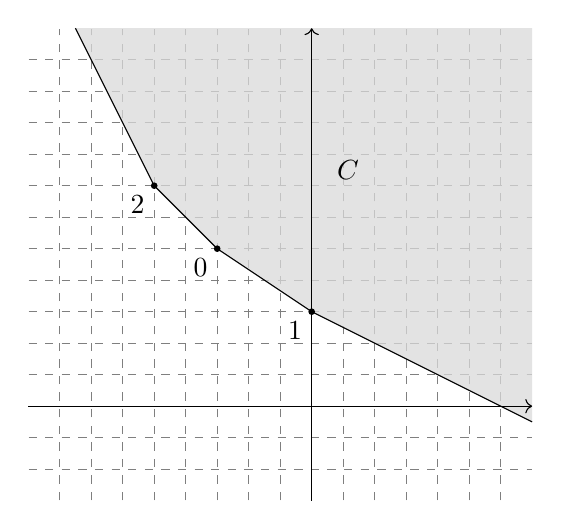
\begin{tikzpicture}[scale=0.40]
\draw (-5.99,-4.99)[dashed, opacity=0.5] grid (9.99,9.99);
%\fill[fill=blue!30, opacity=0.50] (-6,10)--(-6,8)--(-3,2)--(10,-4.5)--(10,10);
%\draw (-4.5,10)--(-1,3);
%\draw (-1,3)--(10,-2.5);
\fill[fill=gray!30, opacity=0.75] (-4.5,10)--(-2,5)--(0,3)--(3,1)--(10,-2.5)--(10,10);
\draw[->] (-6,-2) -- (10,-2);
\draw [->] (3,-5) -- (3,10);
\draw (-4.5,10) -- (-2,5);
\draw (-2,5)--(0,3);
\draw (0,3)--(3,1);
\draw (3,1)--(10,-2.5);
\draw (3.5,5.5) node[right] {$C$};
\draw (-2,5) node[below left] {2};
\draw (0,3) node[below left] {0};
\draw (3,1) node[below left] {1};
\fill (3,1) circle[radius=3pt];
\fill (0,3) circle[radius=3pt];
\fill (-2,5) circle[radius=3pt];
\end{tikzpicture}
\end{center}
The element $ \textup{Conv}(\subset, \T)_{\{e_i\}} (C)$ is equal to $((-5,7);2) \in \textup{Conv}(\rho, \T)_{\{e_i + \tau \mid i \in [m]\}}$:
\begin{center}
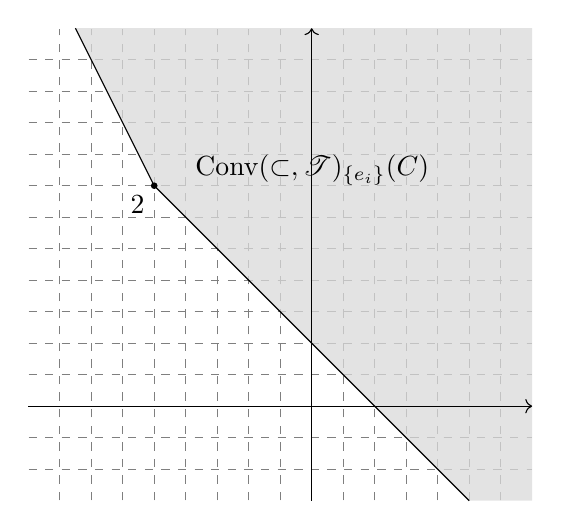
\begin{tikzpicture}[scale=0.40]
\draw (-5.99,-4.99)[dashed, opacity=0.5] grid (9.99,9.99);
%\fill[fill=blue!30, opacity=0.50] (-6,10)--(-6,8)--(-3,2)--(4,-5)--(10,-5)--(10,10);
%\draw (-6,8)--(-3,2);
%\draw (-3,2)--(4,-5);
\fill[fill=gray!30, opacity=0.75] (-4.5,10)--(-2,5)--(8,-5)--(10,-5)--(10,10);
\draw[->] (-6,-2) -- (10,-2);
\draw [->] (3,-5) -- (3,10);
\draw (-4.5,10)--(-2,5);
\draw (-2,5)--(8,-5);
\draw (-1,5.5) node[right] {$ \textup{Conv}(\subset, \T)_{\{e_i\}} (C)$};
\draw (-2,5) node[below left] {2};
\fill (-2,5) circle[radius=3pt];
\end{tikzpicture}
\end{center}
\end{ex}
\begin{oss}
Note that, in the example above, as the image of $C$ in $\textup{Conv}(\rho, \T)_{\{e_i\}}$ is a translate of $\rho$, it is invertible. In fact, this is always true, eventually: for any cone $\tau$ and $C \in \textup{Conv}(\tau, \T)_{\{e_i\}}$, there exits a cone $\tau \subset \rho \subset H_\omega $ such that the image of $C$ in $\textup{Conv}(\rho, \T)_{\{e_i\}}$ is invertible. We will make this into a formal statement in Proposition \ref{prop:colimit-cones}.
Furthermore, by changing the vector $\omega$, we can choose any of the vertices of $C$ to be the only surviving one. Indeed, let $\omega=(1, \sqrt{2})$, then $(0,3)$ is the only vertex of $ \textup{Conv}(\subset, \T)_{\{e_i\}} (C)$ with respect to the inclusion $\tau \subset \textup{pos} \langle (3,-1), (2,-1) \rangle \subset H_\omega$, and analogously, choosing $\omega = (\sqrt{2}/2, 1)$, $(-3,5)$ is the only vertex of $ \textup{Conv}(\subset, \T)_{\{e_i\}} (C)$ with respect to the inclusion $\tau \subset \textup{pos} \langle (-1,1), (3,-2) \rangle \subset H_\omega$.
\end{oss}
\begin{prop} \label{prop:colimit-cones}
The following isomorphism of $\T$-algebras holds:
\[
    \colim_{\mathbf{Cones}_\omega} \textup{Conv}(-, \T)_{\{e_i\}}  \cong \textup{Lead}_\omega(\Z^m, \T).
\]
\end{prop}
\begin{proof}
    Firstly, the $\T$-algebra $\textup{Lead}_\omega(\Z^m, \T)$ is a co-cone for the functor $ \textup{Conv}(-, \T)_{\{e_i\}} $ via the family of $\T$-algebra morphisms $\{\mu_\tau \co \textup{Conv}(\tau, \T)_{\{e_i\}} \rightarrow \textup{Lead}_\omega(\Z^m, \T)\}_{\tau}$ defined by:
    \begin{equation}\label{eq:family-cocone}
        C :=((\jj_i; \alpha_i))_{i \in [\ell]} \mapsto (\jj_{\overline i}:= \min_{\preceq_{\omega}}\{\jj_i \mid i \in [\ell]\}, \alpha_{\overline i}).
    \end{equation}
    In fact, given any two cones $\tau \subset \rho$, the diagram 
    \[
        \begin{tikzcd}
            \textup{Conv}(\tau, \T)_{\{e_i\}} 
            \arrow[rr, " \textup{Conv}(\subset{,} \T)_{\{e_i\}} "]  
            \arrow[dr, swap, "\mu_\tau"]
            & &
            \textup{Conv}(\rho, \T)_{\{e_i\}}  
            \arrow[dl, "\mu_\rho"]
            \\
             & \textup{Lead}_\omega(\Z^m, \T) & 
        \end{tikzcd}
    \]
    commutes. This is equivalent to saying that given an element $C$ in $\textup{Conv}(\tau, \T)_{\{e_i\}}$, the vertex $\jj$ of $C$ attaining the minimum with respect to $\preceq_\omega$ is a vertex of the image of $C$ via any map $\textup{Conv}(\subset, \T)_{\{e_i\}} $. This indeed holds: since $\jj$ is the only vertex of $C$ lying on the hyperplane $\jj + \{x \in \R^m \mid \langle x, \omega \rangle = 0\}$ and all the others lie in $ \jj + \{x \in \R^m \mid \langle x, \omega \rangle > 0\}$, we have that $\jj$ is a vertex of the convex hull of $C$ with respect to any cone $\tau \subset \rho \subset H_\omega$.

    Thus, there is a unique morphism of $\T$-algebras
    \[
    \mu \co \colim_{\mathbf{Cones}_\omega} \textup{Conv}(-, \T)_{\{e_i\}}  \rightarrow  \textup{Lead}_\omega(\Z^m, \T).
    \]
    Since, for instance, the map $\mu_{(\R_{\ge 0})^m}$ is surjective, as the element $(\jj, \alpha)$ is the image of $C = ((\jj, \alpha)) \in  \textup{Conv}((\R_{\ge 0})^m, \T)_{\{e_i\}}$, we have that $\mu$ is surjective. For the injectivity, given two cones $\tau_1, \tau_2 \subset H_\omega$ and elements $C_1 \in \textup{Conv}(\tau_1, \T)_{\{e_i \}}$ and $C_2 \in \textup{Conv}(\tau_2, \T)_{\{e_i \}}$ such that 
    \[
        \mu_{\tau_1}(C_1) = \mu_{\tau_2}(C_2) = (\jj, \alpha) \in \textup{Lead}_\omega(\Z^m, \T), 
    \]
    by definition of the maps $\mu_{\tau_i}$ selecting the minimum of the vertices with respect to $\preceq_\omega$, there exists a cone $\tau_1, \tau_2 \subset \rho \subset H_\omega$ such that
    \[
        \textup{Conv}(\subset, \T)_{\{e_i \}}(C_1) = \textup{Conv}(\subset, \T)_{\{e_i \}}(C_2) = ((\jj, \alpha)) \in \textup{Conv}(\rho, \T)_{\{e_i \}}
    \]
    thus $C_1$ and $C_2$ are identified in the colimit, and the map $\mu$ is injective, thus giving the desired isomorphism.
\end{proof}

The semiring $\textup{Lead}_\omega(\Z^m, \T)$ is a semifield and by Proposition \ref{prop:colimit-cones} above we have a valuation 
\begin{equation} \label{eq:v-omega}
    v_\omega \co K(\!(t_1, \dots , t_m)\!)_\omega \rightarrow \textup{Lead}_\omega(\Z^m, \T).
\end{equation}
defined by sending a series $A=\sum_{\jj \in \Z^m} a_\jj t^\jj$ to $(\overline \jj:=\min_{\preceq_\omega}\supp( A), v_K(a_{\overline \jj} ))$, that becomes surjective restricting the weights to the value group $\Gamma_K$ of $v_K$. Notice that the restriction of $v_\omega$ to $\pkcone \tau$ for any cone $\tau \subset H_\omega$, is the valuation $v_{\tau, \omega}$ of Example \ref{ex:omega-val-tau}. 

If the valuation $v_K \co K \rightarrow \T$ has a section then the corresponding extended valuation $v_\omega \co K(\!(t_1, \dots , t_m)\!)_\omega \rightarrow \textup{Lead}_\omega(\Z^m, \widetilde{\Gamma}_K)$ has a section as well. Indeed, denoting as $\pi_K$ a uniformizer for $v_K$, the map 
\begin{align*}
    \varphi_\omega \co \textup{Lead}_\omega(\Z^m, \widetilde{\Gamma}_K) &\rightarrow K(\!(t_1, \dots t_m)\!)_\omega \\
   (\jj,\alpha) &\mapsto \pi_K^{\alpha} t^{\jj} 
\end{align*}
is a section for the valuation $v_\omega$, and we will drop the subscript $\omega$ when it is clear from the context. Given a cone $\tau \subset H_\omega$, let again $v_\tau$ be the valuation 
\[
    v_\tau \co \pkcone \tau _{t_1, \dots t_m} \rightarrow \textup{Conv}(\tau, \T)_{\{e_i \}}
\]
extending the valuation $v_\tau$ of Example \ref{ex:conv-vals}. It is easy to check that the valuation ring with respect to $v_\tau$ and the maximal ideal of this ring are the following: 
\begin{align*}
    R_{v_\tau} :&= \{A \in \pkcone \tau _{t_1, \dots t_m} \mid v(x) \preceq (0_{\Z^m},0)\} = 
    \left \{A =\sum_{\jj \in \Z^m} a_\jj t^\jj \in \pkcone \tau \mid a_{0_{\Z^m}} \in R_K \right  \}, 
    \\
    \mathfrak m _{v_\tau} :&= \{A \in \pkcone \tau _{t_1, \dots t_m} \mid v(x) \prec (0_{\Z^m},0)\} =
    \left \{A =\sum_{\jj \in \Z^m} a_\jj t^\jj \in \pkcone \tau \mid  a_{0_{\Z^m}} \in \mathfrak m_K \right \}, 
\end{align*}   
and the residue field $ R_{v_\tau}/\mathfrak m _{v_\tau}$ is isomorphic to $k=R_K/\mathfrak m_K$.
From the equalities above, and from the definition of the field $K(\!(t_1, \dots t_m)\!)_\omega$, the following hold:
\begin{align*}
    R_{v_\omega} :&= \{A \in K(\!(t_1, \dots t_m)\!)_\omega \mid v_\omega(x) \preceq (0_{\Z^m},0)\} = \bigcup_{\tau \subset H_\omega} R_{v_\tau} =
    \\
    &= \left \{A \in K(\!(t_1, \dots t_m)\!)_\omega \mid  A \in R_{v_\tau} \text{ for some cone } \tau \subset H_\omega \right \} = 
    \\
    &= \left \{ A=\sum_{\jj \in \Z^m} a_\jj t^\jj \in K(\!(t_1, \dots t_m)\!)_\omega \mid  \supp(A) \subset H_\omega \text{ and } a_{0_{\Z^m}} \in R_K \right \} ;
    \\
    \mathfrak m _{v_\omega} :&= \{A \in K(\!(t_1, \dots , t_m)\!)_\omega \mid v_\omega(x) \prec (0_{\Z^m},0)\} = \bigcup_{\tau \subset H_\omega} \mathfrak m_{v_\tau} =
    \\
    &= \left \{A \in K(\!(t_1, \dots t_m)\!)_\omega \mid A \in \mathfrak m_{v_\tau} \text{ for some cone } \tau \subset H_\omega \right \} =
    \\
    &= \left \{A=\sum_{\jj \in \Z^m} a_\jj t^\jj \in K(\!(t_1, \dots t_m)\!)_\omega \mid  \supp(A) \subset H_\omega \text{ and } a_{0_{\Z^m}} \in \mathfrak m_K \right \}.
\end{align*}   
The residue field $R_{v_\omega}/\mathfrak m _{v_\omega}$ is isomorphic to $k$. We will write $\overline A \in k$ for the residue class of an element $A \in R_{v_\omega}$ and if $f \in \diff {K(\!(t_1 , \dots , t_m)\!)_\omega}{n}$ has coefficients in $R_{v_\omega}$, let $\overline f \in \diff k n$ be the differential polynomial obtained by taking the residue class of its coefficients.

Given $S := (S_1, \dots , S_n) \in \ptt m ^n_{v_K}$, the elements $\Phi_m(d^\jj S_i)$ and $\trop_v(f)(S)$ live in $\textup{Conv}_m(\T) \subset \textup{Conv}_m(\T)_{\{e_i\}}$, thus we can look at their image via the map $\mu_m :=\mu_{(\R_{\ge 0})^m}$ of \ref{eq:family-cocone}. For every $\jj \in \N^m$ such that $\Phi_m(d^\jj S_i)\neq \emptyset$ let 
\[
(\fatg_{i, \jj}, \alpha_{i, \jj}) := \mu_m(\Phi_m(d^\jj S_i)).
\]
In the same way, if $\trop_v(f)(S) \neq \emptyset$, let $(\hh, \alpha) :=\mu_m( \trop_v(f)(S))$. 
\begin{comment}\begin{oss}\label{oss:bring-back-to-pos-orthant}
Given $C \in \textup{Conv}_m(\T)$ there is a canonical way to associate to $C$ an element in $\{D \in  \textup{Conv}_m(\T) \mid D \preceq 1_{\textup{Conv}_m(\T)}\}$. Indeed, if $C=((\hh_1;\alpha_1),   \dots ,( \hh_\ell; \alpha_\ell))$ with $\hh_i = (h_{i,1}, \dots , h_{i,m}) \in \Z^m$ for every $i$, then 
\[
C \preceq (\hh ; \alpha) :=
 \left ( \left (\min_{i \in \{1 , \dots , \ell\}} h_{i,1}, \dots , \min_{i \in \{1 , \dots , \ell\}} h_{i,m} \right )  ; \min_{i \in \{1 , \dots , \ell\}} \alpha_i \right ),
\]
thus $(-\hh ; -\alpha) \odot C \preceq 1_{\textup{Conv}_m(\T)}$.
Notice that for $m=1$, $C=(h, \alpha) \in \T_2$ and the construction above trivially retrieves $C$ itself.
\end{oss}
\begin{ex}
Let $C \in \textup{Conv}_2(\T)$ be the following weighted convex hull: 
\[
    C=(((-1,3);2), ((1,-1);-1), ((4,-2);0))
\]
which corresponds to the following picture:
\begin{center}
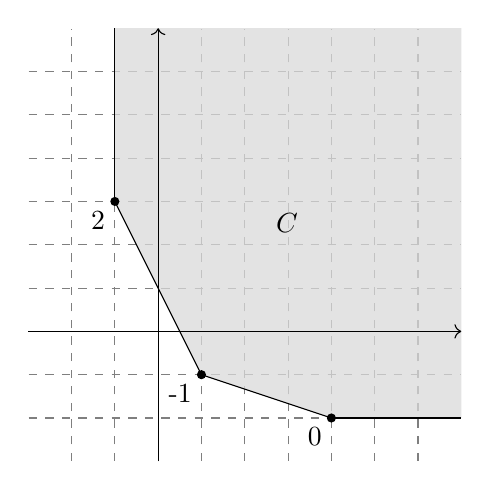
\begin{tikzpicture}[scale=0.55]
\draw (-2.99,-2.99)[dashed, opacity=0.5] grid (6.99,6.99);
\fill[fill=gray!30, opacity=0.75] (-1,7)--(-1,3)--(1,-1)--(4,-2)--(7,-2)--(7,7);
\draw[->] (-3,0) -- (7,0);
\draw [->] (0,-3) -- (0,7);
\draw (-1,7) -- (-1,3);
\draw (-1,3)--(1,-1);
\draw (1,-1)--(4,-2);
\draw (4,-2)--(7,-2);
\draw (2.5,2.5) node[right] {$C$};
\draw (-1,3) node[below left] {2};
\draw (1,-1) node[below left] {-1};
\draw (4,-2) node[below left] {0};
\fill (-1,3) circle[radius=3pt];
\fill (1,-1) circle[radius=3pt];
\fill (4,-2) circle[radius=3pt];
\end{tikzpicture}
\end{center}
then, following the construction illustrated in the Remark above, $C \preceq ((-1,-2);-1)$, and 
\[
    C \odot ((1,2);1) = (((0,5);3), ((2,1);0), ((5,0);1)) \preceq 1_{\textup{Conv}_2(\T)}.
\]
The weighted convex hull $C \odot ((1,2);1) $ is depicted below:
\begin{center}
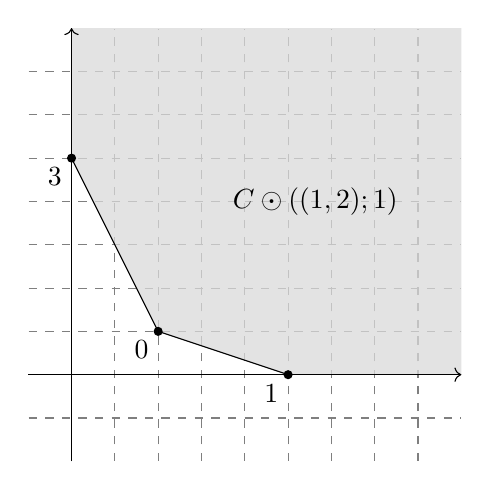
\begin{tikzpicture}[scale=0.55]
\draw (-2.99,-2.99)[dashed, opacity=0.5] grid (6.99,6.99);
\fill[fill=gray!30, opacity=0.75] (-2,7)--(-2,4)--(0,0)--(3,-1)--(7,-1)--(7,7);
\draw[->] (-3,-1) -- (7,-1);
\draw [->] (-2,-3) -- (-2,7);
\draw (-2,7) -- (-2,4);
\draw (0,0) -- (-2,4);
\draw (0,0)--(3,-1);
\draw (3,-1)--(6,-1);
\draw (7,-1)--(6,-1);
\draw (1.5,3) node[right] {$C \odot ((1,2);1) $};
\draw (-2,4) node[below left] {3};
\draw (0,0) node[below left] {0};
\draw (3,-1) node[below left] {1};
\fill (-2,4) circle[radius=3pt];
\fill (0,0) circle[radius=3pt];
\fill (3,-1) circle[radius=3pt];
\end{tikzpicture}
\end{center}
\end{ex}
Let $(\hh; \alpha)$ the result of the construction explained in Remark \ref{oss:bring-back-to-pos-orthant} for $C =\trop_v(f)(S)$ and let $C_{i,\jj} := \Phi_m(d^\jj S_i)$. We are now ready to define the initial form of $f$ with respect to $S$.
\end{comment}
\begin{defin} \label{definition:initial}
    Let $S \in \ptt m ^n_{v_K}$ and $f \in \diff {K(\!(t_1, \dots , t_m)\!)_\omega}{n}$. Writing $f = \sum_{\lambda \in \Lambda} A_\lambda \prod_{i,\jj}(x_i^{(\jj)})^{\lambda_{i,\jj}}$ as in Section \ref{section:theorem}, we define:
    \[
    h_{(S,\omega)} := \varphi  \left ( (-\hh; -\alpha) \right ) \sum_{\lambda \in \Lambda} A_\lambda \prod_{i,\jj} \left ( \varphi  \left ( ( \fatg_{i,\jj}, \alpha_{i,\jj} ) \right )  x_i^{(\jj)} \right ) ^{\lambda_{i,\jj}} \in \diff {K(\!(t_1, \dots , t_m)\!)_\omega} n.
    \] 
    The differential polynomial $h_S$ has coefficients in $R_{v_\omega}$.
    The initial form $in_{(S,\omega)}(f) \in \diff k n$ of $f$ with respect to $(S, \omega)$ is defined as follows:
    \[
    in_{(S, \omega)}(f) :=
        \begin{cases}
            \overline {h_{(S, \omega)}}   & \text{if $\trop_v(f)(S) \neq \infty$} \\
            & \\
            0 & \text{if $\trop_v(f)(S) = \infty$}
        \end{cases}
    \]
\end{defin}

\begin{oss}\label{oss:initial}
    There is at least one coefficient in the differential polynomial $h_S$ above with valuation $(0_{\Z^m},0)=1_{\textup{Lead}_\omega(\Z^m,\T)}$ with respect to $v_\omega$, thus $in_{(S, \omega)}(f) = 0$ if and only if $\trop_v(f)(S) = \emptyset \in \textup{Conv}_m(\T)$. Indeed
    \begin{align*}
            h_{(S, \omega)}  :&= \varphi  \left ( (-\hh; -\alpha) \right ) \sum_{\lambda \in \Lambda} A_\lambda \prod_{i,\jj} \left ( \varphi  \left ( ( \fatg_{i,\jj}, \alpha_{i,\jj} ) \right )  x_i^{(\jj)} \right ) ^{\lambda_{i,\jj}} = \\
            & = \varphi  \left ( (-\hh, - \alpha)  \right ) \sum_{\lambda \in \Lambda} A_\lambda \prod_{i,\jj}  \varphi  \left ( (\fatg_{i,\jj}, \alpha_{i,\jj})  \right )   ^{\lambda_{i,\jj}}  x^\lambda
	\end{align*}
    thus the $v_\omega$ valuation of the coefficient of $x^\lambda$ in $h_S$ is
    \[
    (-\hh, -\alpha) \odot v_\omega(A_\lambda) \odot \bigodot_{i,\jj} (\fatg_{i,\jj}, \alpha_{i,\jj})^{\odot \lambda_{i,\jj}}. 
    \]
    Given that $(\hh, \alpha) = \mu_m( \trop_v(f)(S))$ is the minimum of the elements $v_\omega(A_\lambda) \odot \bigodot_{i,\jj} (\fatg_{i,\jj}, \alpha_{i,\jj})^{\odot \lambda_{i,\jj}}$, this proves that the coefficients of the polynomial $h_S$ are elements of $R_{v_\omega}$. In particular, the only coefficients with valuation $(0_{\Z^m},0)$ are those of the monomials where $(\hh, \alpha)$ is attained.
\end{oss}
\begin{oss}
    Notice that for $m=1$, the initial form of a differential polynomial (and so the initial ideal of a differential ideal, see Definition \ref{def:initial-ideal}) depends only on $S$, as in this case, up to scaling, there is only a choice for $\omega$.
\end{oss}
\begin{comment}
When $m > 1$, the analogous statement would be that there is at least one coefficient in the differential polynomial $h_S$ with valuation $1_{\textup{Conv}_m(\T)}$, which would imply that $in_S(f) = 0$ if and only if $\trop_v(f)(S) = \emptyset$. This unfortunately fails, even in the case of trivial valuation, as the following example shows. 

\begin{ex}\label{ex:initial-fails}
Let $m=2$ and $f = (t_1 + t_2)x + x^{(1,0)} \in \C[\![t_1, t_2]\!]\{x\}$. Let $C = v(t_1 + t_2) = ((1,0),(0,1)) \in \textup{Conv}_2(\B)$ and $S = 0 +t_1^2 + t_1t_2 \in \B[\![t_1,t_2]\!]$. Then we have
\[
    \trop_v(f)=Cx + 1_{\textup{Conv}_2(\B)}x^{(1,0)} \in \textup{Conv}_2(\B)\{x\}_{\textit{basic}}
\]
and 
\begin{align*} 
    \trop_v(f)(S)  & =C \odot \Phi_2(S) + 1_{\textup{Conv}_2(\B)} \odot \Phi_2(d^{(1,0)}S) =
    \\
    & = C \odot 1_{\textup{Conv}_2(\B)} \oplus 1_{\textup{Conv}_2(\B)} \odot C = C.
\end{align*}
Thus, we have the following
\begin{align*} 
    h_S  & = \varphi(1_{\textup{Conv}_2(\B)}) \left ( (t_1 + t_2) \cdot \varphi(1_{\textup{Conv}_2(\B)}) x + 1 \cdot \varphi(C) x^{(1,0)}\right) =
    \\
    & = 1 \cdot \left ( (t_1 + t_2) \cdot 1 \cdot x + 1 \cdot (t_1 + t_2)x^{(1,0)}\right) 
    \\
    & =  (t_1 + t_2) x + (t_1 + t_2)x^{(1,0)}
\end{align*}
and clearly $\overline{h_S} = 0$ even though $\trop(f)(S) = C \neq \emptyset$.
\end{ex}
In view of Example \ref{ex:initial-fails} above, from here on we work only in the case $m=1$.
\end{comment}
\begin{defin} \label{def:initial-ideal}
    Let $I \subseteq \diff {\pkk m} n$ be a differential ideal, then the initial ideal of $I$ with respect to $(S, \omega)$ is the (algebraic) ideal: 
    \[
        In_{(S, \omega)}(I):=\langle in_{(S, \omega)}(f) \mid f \in I \rangle \subseteq \diff k n
    \]
\end{defin}

\begin{oss}
Similarly to what already noticed in \cite[Example 3.5]{FT20}, given $f \in I$ in general we have 
\[d(in_{(S,\omega)}(f)) \neq in_{(S, \omega)}(df).\]
\end{oss}
We now generalize \cite[Lemma 2.6]{hugao} and \cite[Lemma 3.8]{FT20} to the nontrivially valued multivariate setting:
\begin{lem} \label{lemma:initial}
    Let $S \in \ptt m^n_{v_K}$ and $I \subseteq \diff {R_m} n$ be a differential ideal, for every $F \in In_{(S, \omega)}(I)$ there exists $f \in I$ such that $ F = in_{(S, \omega)}(f)$. 
\end{lem}
\begin{proof}
    As in Definition \ref{definition:initial}, for all $\jj \in \N^m$ such that $\Phi_m(d^\jj S_i)\neq \emptyset$, let 
    \[
    (\fatg_{i,\jj}, \alpha_{i,\jj}) := \mu_m(\Phi_m(d^\jj S_i)).
    \]
    Given $F \in In_{(S, \omega)}(I)$, we can write it as  $\sum_{\lambda \in \Lambda} a_\lambda x^\lambda in_{(S, \omega)}(f_\lambda)$ for some $a_\lambda \in k$ and $f_\lambda \in I$. Let 
    \[
        (\hh_\lambda, \alpha_\lambda):=\mu_{m}(\trop_v(f_\lambda)(S)) \quad \quad 
        (\hh'_\lambda, \alpha'_\lambda):= (\hh_\lambda, \alpha_\lambda) \odot \bigodot_{i,\jj}  (\fatg_{i,\jj}, \alpha_{i,\jj})^{\odot\lambda_{i,\jj}}
    \]
    and 
    \[
        f := \sum_{\lambda \in \Lambda} A_\lambda \varphi \left ((-\hh_\lambda, -\alpha_\lambda) \right ) x^\lambda f_\lambda
    \]
    for elements $A_\lambda \in \pkk m$ such that $v(A_\lambda) = v_\omega(A_\lambda) = (0_{\Z^m},0)$ and $\overline {A_\lambda} = a_\lambda$: notice that $\mu_m(\trop_{v}(f)(S)) = (0_{\Z^m},0)$.
    
    We claim that the initial form of $f$ with respect to $(S, \omega)$ is $F$. Let us compute $in_{(S,\omega)}(f)$:
    \begin{align*}
    in_{(S,\omega)}(f) & = \overline {h_{(S,\omega)}} = \\
    & = \overline { \sum_{\lambda \in \Lambda} A_\lambda \varphi \left ((-\hh'_\lambda, -\alpha'_\lambda) \right ) \prod_{i,\jj} \left ( \varphi  \left ( (\fatg_{i,\jj}, \alpha_{i,\jj})  \right )  x_i^{(\jj)} \right) ^{\lambda_{i,\jj}} f_\lambda \left ( \varphi \left ( (\fatg_{i,\jj}, \alpha_{i,\jj})  \right )  x_i^{(\jj)} \right)} = \\
    & =  \overline{ \sum_{\lambda \in \Lambda} A_\lambda \varphi \left ((-\hh'_\lambda, -\alpha'_\lambda) \right ) \prod_{i,\jj} \left ( \varphi  \left ( (\fatg_{i,\jj}, \alpha_{i,\jj})  \right )  \right ) ^{\lambda_{i,\jj}}  x^\lambda f_\lambda \left ( \varphi \left ( (\fatg_{i,\jj}, \alpha_{i,\jj})  \right )  x_i^{(\jj)} \right ) }= \\
    & = \sum_{\lambda \in \Lambda} \overline{A_\lambda  \varphi \left ((-\hh_\lambda, -\alpha_\lambda) \right )  f_\lambda \left ( \varphi \left ((\fatg_{i,\jj}, \alpha_{i,\jj})  \right )  x_i^{(\jj)} \right)  x^\lambda }   .\\
    \end{align*}
    As $\overline{A_\lambda} = a_\lambda$ by definition and $\overline{ \varphi \left ((-\hh_\lambda, -\alpha_\lambda) \right ) f_\lambda \left ( \varphi \left ((\fatg_{i,\jj}, \alpha_{i,\jj})  \right )  x_i^{(\jj)} \right) }$ is the initial form of $f_\lambda$ with respect to $(S,\omega)$, we have
    \[
        in_{(S, \omega)}(f) = \sum_{\lambda \in \Lambda} a_\lambda x^\lambda in_{(S, \omega)}(f_\lambda) = F
    \]
    that proves the claim.
\end{proof}
Since given any vector $\omega \in (\R_{>0})^m$ with rationally independent coordinates we have that $R_m = \pkk m \subset K(\!(t_1, \dots t_m)\!)_\omega$, we can consider how the initial of $I$ with respect to $(S,\omega)$ varies by varying the vector $\omega$. Let 
\[
     \Sigma_\omega :=\{S \in \widetilde{\Gamma}_K[\![t_1, \dots t_m]\!]^n_{v_K} \mid In_{(S, \omega)}(I) \text{ does not contain a monomial}\} 
\]
then we have:

\begin{teorema}\label{theorem:fundamental-initial}
Under the same hypothesis of Theorem \ref{theorem:fundamental}, the following equalities hold:
\[
         \trop_{\tilde v}(\textup{Sol}_{R_m}(I)) =
         \textup{Sol}_{\mathbf \Gamma}(\trop_{v} (I)) 
         =
        \bigcap_{\substack{\omega \in (\R_{>0})^m
                \\ 
                \text{with $\Q$-ind. coords}
                }} \Sigma_\omega
\]
\end{teorema}

\begin{proof}
        We will prove the equality: 
        \begin{equation} \label{eq:solutions-initial}
        \textup{Sol}_{\mathbf \Gamma}(\trop_{v} (I)) =
        \bigcap_{\substack{\omega \in (\R_{>0})^m
                \\ 
                \text{with $\Q$-ind. coords}
                }} \Sigma_\omega.
        \end{equation}
        Let us start from the "$\subseteq$" inclusion. Given $S \in \textup{Sol}_{\mathbf \Gamma}(\trop_{v} (I))$, by definition, for every $f \in I$, either $\trop_v(f)(S)=\emptyset$ or each of its vertices is a vertex of the evaluation at $S$ of at least two monomials, with the same weight it carries in $\trop_v(f)(S)$. 
        
        For any vertex $\jj$ of $\trop_v(f)(S)$, let $\alpha$ be its weight and choose $\omega_\jj \in (\R_{>0})^m$ with rationally independent coordinates, such that the image of $\trop_v(f)(S)$ via the map
        \[
            \mu_{m,\jj} \co \textup{Conv}_m(\T)_{\{e_i\}} \rightarrow \textup{Lead}_\omega(\Z^m, \T)
        \]
        is equal to $(\jj, \alpha)$, i.e.\ $\jj$ minimizes $\langle \jj, \omega \rangle$ among the vertices of $\trop_v(f)(S)$.
        From Remark \ref{oss:initial} we know that for every $f \in I$ the initial $in_{(S, \omega)}(f)$ is either 0 or it is at least a binomial. The ideal $In_{(S, \omega)}(I)$ cannot contain any monomial: indeed if $F \in In_{(S, \omega)}(I)$ is a monomial, then from Lemma \ref{lemma:initial}, there exists $f \in I$ such that $in_{(S, \omega)}(f) = F$ is a monomial, and that contradicts the fact that $S$ is a solution for $\trop_{v} (I)$.
        
        For what concerns the opposite inclusion: assume $S$ is not in $\textup{Sol}_{\mathbf \Gamma}(\trop_{v} (I))$. Then there would exist a polynomial $f \in I$ and a weighted vertex $(\jj, \alpha)$ of $\trop_v(f)(S)$ that appears as a vertex of the evaluation at $S$ of exactly one of the monomials of $f$. Thus, choosing $\omega_\jj$ such that $\jj$ minimizes $\langle \jj, \omega \rangle$ among the vertices of $\trop_v(f)(S)$ as above, thanks to the discussion of Remark \ref{oss:initial}, we have that $in_{(S, \omega)}(f)$ is a monomial. Thus $S$ does not belong to the right hand side of \ref{eq:solutions-initial}. This concludes the proof.
\end{proof}

\begin{comment}
\begin{ex}
Fix a prime number $p$ and consider the equation $f = x' - p \zeta t^{p-1} x  \in \C_p[\![t]\!]\{x\}$ that we will introduce in Example \ref{ex:p-adic-diffeq} and let $S = \sum_{n=0}^\infty a_n t^n \in (\Q \cup \{\infty\})[\![t]\!]_{v_p}$ be the tropical power series with coefficients
\begin{equation*}
a_n =
\begin{cases*}
\infty & if $p \ndiv n$ \\
\frac{m}{p-1} - v_p(m!)  & if $n = mp$.
\end{cases*}
\end{equation*}
As we will prove in the aformentioned example, $S$ is a solution for the tropicalization of the differential ideal $I$ generated by $f$. Thus the initial ideal $In_S((f))$ does not contain monomials. Let us compute the initial of $f$ with respect to $S$. The tropicalization of $f$ is $\trop_v(f) = x' + (p-1 \text{, } p/(p-1))x$. The evaluation of $\trop_v(f)$ in $S$ gives  $(p-1 \text{, } p/(p-1))$ attained at both monomials. Thus:
\[
    in_S(f) = x' + x \in \diff {\overline{\mathbb F _p}} n.
\]
\end{ex}
\end{comment}

\begin{oss}
The theory presented above presents interesting links with that developed in \cite{initialslara}. The first author intends to investigate them further. 
\end{oss}

\begin{ex}
    Let $m=2$, $n=1$ and $p=2$. Let $\C_2[\![t_1, t_2]\!]$ be endowed with the differentially enhanced valuation:
    \[
    \begin{tikzcd}
        & \T[\![t_1, t_2]\!] _{v_2} \arrow[d, "\Phi_2"] \\
        \C_2[\![t_1, t_2]\!]  \arrow[ur, "\widetilde{v}"] \arrow[r,swap,"v"] & \textup{Conv}_2(\T) 
    \end{tikzcd}
    \]
as in point (4) of Example \ref{ex:diff-enhancements}. Consider the following differential polynomial in $\C_2[\![t_1, t_2]\!]\{x\}$: 
    \[
        F:=\left(6t_1+\frac{5}{2}t_2 \right) (x^{(0,1)})^2 + 3t_1t_2x^{(2,3)} + (4t_1t_2^3 + t_1^2t_2 - 4t_1^3)x^{(1,0)}.
    \]
The tropicalization of $F$ is 
\[\trop_v(F)=    
    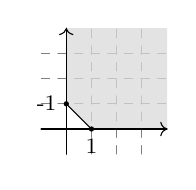
\begin{tikzpicture}        
        [line cap=round,line    join=round,x=1cm,y=1cm,baseline={0.5cm-0.5*height("$=$")}, scale=0.32]
        \draw (-0.99,-0.99)[dashed, opacity=0.5] grid (3.99,3.99);
        \fill[fill=gray!30, opacity=0.75] (0,4)--(0,1)--(1,0)--(4,0)--(4,4);
        \draw[->] (-1,0) -- (4,0);
        \draw [->] (0,-1) -- (0,4);
        \draw (0,4) -- (0,1);
        \draw (0,1)--(1,0);
        \draw (1,0)--(4,0);
        \draw (1,0) node[below] {\footnotesize 1};
        \draw (0,1) node[left]{\footnotesize -1};
        \fill (1,0) circle[radius=3pt];
        \fill (0,1) circle[radius=3pt];
    \end{tikzpicture}
        (x^{(0,1)})^2 +
    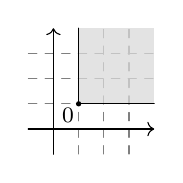
\begin{tikzpicture}        
        [line cap=round,line    join=round,x=1cm,y=1cm,baseline={0.5cm -0.5*height("$=$")}, scale=0.32]
        \draw (-0.99,-0.99)[dashed, opacity=0.5] grid (3.99,3.99);
        \fill[fill=gray!30, opacity=0.75] (1,4)--(1,1)--(4,1)--(4,4);
        \draw[->] (-1,0) -- (4,0);
        \draw [->] (0,-1) -- (0,4);
        \draw (1,4) -- (1,1);
        \draw (1,1)--(4,1);
        \draw (1.2,1.2) node[below left ] {\footnotesize 0};
        \fill (1,1) circle[radius=3pt];
    \end{tikzpicture}
     x^{(2,3)} +
    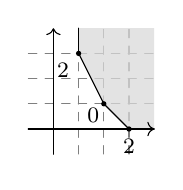
\begin{tikzpicture}        
         [line cap=round,line    join=round,x=1cm,y=1cm,baseline={0.5cm-0.5*height("$=$")}, scale=0.32]
        \draw (-0.99,-0.99)[dashed, opacity=0.5] grid (3.99,3.99);
        \fill[fill=gray!30, opacity=0.75] (1,4)--(1,3)--(2,1)--(3,0)--(4,0)--(4,4);
        \draw[->] (-1,0) -- (4,0);
        \draw [->] (0,-1) -- (0,4);
        \draw (1,4) -- (1,3);
        \draw (1,3)--(2,1);
        \draw (2,1)--(3,0);
        \draw (3,0)--(4,0);
        \draw (1,3) node[below left] { \footnotesize 2};
        \draw (2.2,1.2) node[below left]{ \footnotesize 0};
        \draw (3,0) node[below]{ \footnotesize 2};
        \fill (3,0) circle[radius=3pt];
        \fill (1,3) circle[radius=3pt];
        \fill (2,1) circle[radius=3pt];
    \end{tikzpicture}
    x^{(1,0)} \in \textup{Conv}_2(\T)\{x\}_{\textit{basic}}.
\]
We claim that the tropical power series
\[ 
    S = 1t_1 + 1t_1t_2 +  1t_1^2t_2^5 + (-1)t_1^3t_2^3 \in  \T[\![t_1, t_2]\!] _{v_2}
\]
is a solution for the tropicalization of $F$. Indeed we have: 
\begin{align*}\trop_v(F)(S) & =    
    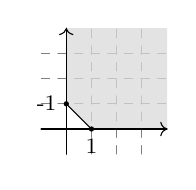
\begin{tikzpicture}        
        [line cap=round,line  join=round,x=1cm,y=1cm,baseline={0.5cm-0.5*height("$=$")}, scale=0.32]
        \draw (-0.99,-0.99)[dashed, opacity=0.5] grid (3.99,3.99);
        \fill[fill=gray!30, opacity=0.75] (0,4)--(0,1)--(1,0)--(4,0)--(4,4);
        \draw[->] (-1,0) -- (4,0);
        \draw [->] (0,-1) -- (0,4);
        \draw (0,4) -- (0,1);
        \draw (0,1)--(1,0);
        \draw (1,0)--(4,0);
        \draw (1,0) node[below] {\footnotesize 1};
        \draw (0,1) node[left]{\footnotesize -1};
        \fill (1,0) circle[radius=3pt];
        \fill (0,1) circle[radius=3pt];
    \end{tikzpicture}
    \odot (\Phi_2(d^{(0,1)}S))^2 \oplus
    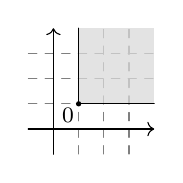
\begin{tikzpicture}        
        [line cap=round,line    join=round,x=1cm,y=1cm,baseline={0.5cm -0.5*height("$=$")}, scale=0.32]
        \draw (-0.99,-0.99)[dashed, opacity=0.5] grid (3.99,3.99);
        \fill[fill=gray!30, opacity=0.75] (1,4)--(1,1)--(4,1)--(4,4);
        \draw[->] (-1,0) -- (4,0);
        \draw [->] (0,-1) -- (0,4);
        \draw (1,4) -- (1,1);
        \draw (1,1)--(4,1);
        \draw (1.2,1.2) node[below left ] {\footnotesize 0};
        \fill (1,1) circle[radius=3pt];
    \end{tikzpicture}
      \odot \Phi_2(d^{(2,3)}S) \oplus
    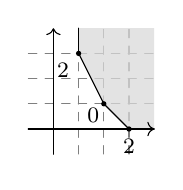
\begin{tikzpicture}        
         [line cap=round,line    join=round,x=1cm,y=1cm,baseline={0.5cm-0.5*height("$=$")}, scale=0.32]
        \draw (-0.99,-0.99)[dashed, opacity=0.5] grid (3.99,3.99);
        \fill[fill=gray!30, opacity=0.75] (1,4)--(1,3)--(2,1)--(3,0)--(4,0)--(4,4);
        \draw[->] (-1,0) -- (4,0);
        \draw [->] (0,-1) -- (0,4);
        \draw (1,4) -- (1,3);
        \draw (1,3)--(2,1);
        \draw (2,1)--(3,0);
        \draw (3,0)--(4,0);
        \draw (1,3) node[below left] { \footnotesize 2};
        \draw (2.2,1.2) node[below left]{ \footnotesize 0};
        \draw (3,0) node[below]{ \footnotesize 2};
        \fill (3,0) circle[radius=3pt];
        \fill (1,3) circle[radius=3pt];
        \fill (2,1) circle[radius=3pt];
    \end{tikzpicture}
    \odot \Phi_2(d^{(1,0)}S)  = \\ 
& =    
    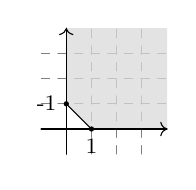
\begin{tikzpicture}        
        [line cap=round,line    join=round,x=1cm,y=1cm,baseline={0.5cm-0.5*height("$=$")}, scale=0.32]
        \draw (-0.99,-0.99)[dashed, opacity=0.5] grid (3.99,3.99);
        \fill[fill=gray!30, opacity=0.75] (0,4)--(0,1)--(1,0)--(4,0)--(4,4);
        \draw[->] (-1,0) -- (4,0);
        \draw [->] (0,-1) -- (0,4);
        \draw (0,4) -- (0,1);
        \draw (0,1)--(1,0);
        \draw (1,0)--(4,0);
        \draw (1,0) node[below] {\footnotesize 1};
        \draw (0,1) node[left]{\footnotesize -1};
        \fill (1,0) circle[radius=3pt];
        \fill (0,1) circle[radius=3pt];
    \end{tikzpicture}
    \odot 
    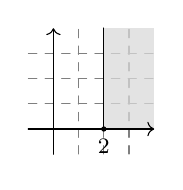
\begin{tikzpicture}        
        [line cap=round,line    join=round,x=1cm,y=1cm,baseline={0.5cm-0.5*height("$=$")}, scale=0.32]
        \draw (-0.99,-0.99)[dashed, opacity=0.5] grid (3.99,3.99);
        \fill[fill=gray!30, opacity=0.75] (2,4)--(2,0)--(4,0)--(4,4);
        \draw[->] (-1,0) -- (4,0);
        \draw [->] (0,-1) -- (0,4);
        \draw (2,4) -- (2,0);
        \draw (2,0)--(2,4);
        \draw (2,0) node[below] {\footnotesize 2};
        \fill (2,0) circle[radius=3pt];
    \end{tikzpicture}
    \oplus
    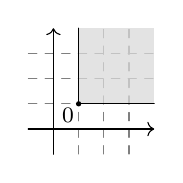
\begin{tikzpicture}        
        [line cap=round,line    join=round,x=1cm,y=1cm,baseline={0.5cm -0.5*height("$=$")}, scale=0.32]
        \draw (-0.99,-0.99)[dashed, opacity=0.5] grid (3.99,3.99);
        \fill[fill=gray!30, opacity=0.75] (1,4)--(1,1)--(4,1)--(4,4);
        \draw[->] (-1,0) -- (4,0);
        \draw [->] (0,-1) -- (0,4);
        \draw (1,4) -- (1,1);
        \draw (1,1)--(4,1);
        \draw (1.2,1.2) node[below left ] {\footnotesize 0};
        \fill (1,1) circle[radius=3pt];
    \end{tikzpicture}
      \odot 
      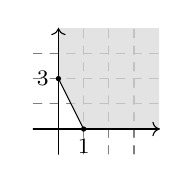
\begin{tikzpicture}        
        [line cap=round,line    join=round,x=1cm,y=1cm,baseline={0.5cm-0.5*height("$=$")}, scale=0.32]
        \draw (-0.99,-0.99)[dashed, opacity=0.5] grid (3.99,3.99);
        \fill[fill=gray!30, opacity=0.75] (0,4)--(0,2)--(1,0)--(4,0)--(4,4);
        \draw[->] (-1,0) -- (4,0);
        \draw [->] (0,-1) -- (0,4);
        \draw (0,4) -- (0,2);
        \draw (0,2)--(1,0);
        \draw (1,0)--(4,0);
        \draw (1,0) node[below] {\footnotesize 1};
        \draw (0,2) node[left]{\footnotesize 3};
        \fill (1,0) circle[radius=3pt];
        \fill (0,2) circle[radius=3pt];
    \end{tikzpicture}
    \oplus
    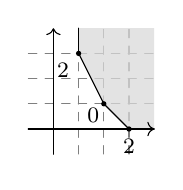
\begin{tikzpicture}        
         [line cap=round,line    join=round,x=1cm,y=1cm,baseline={0.5cm-0.5*height("$=$")}, scale=0.32]
        \draw (-0.99,-0.99)[dashed, opacity=0.5] grid (3.99,3.99);
        \fill[fill=gray!30, opacity=0.75] (1,4)--(1,3)--(2,1)--(3,0)--(4,0)--(4,4);
        \draw[->] (-1,0) -- (4,0);
        \draw [->] (0,-1) -- (0,4);
        \draw (1,4) -- (1,3);
        \draw (1,3)--(2,1);
        \draw (2,1)--(3,0);
        \draw (3,0)--(4,0);
        \draw (1,3) node[below left] { \footnotesize 2};
        \draw (2.2,1.2) node[below left]{ \footnotesize 0};
        \draw (3,0) node[below]{ \footnotesize 2};
        \fill (3,0) circle[radius=3pt];
        \fill (1,3) circle[radius=3pt];
        \fill (2,1) circle[radius=3pt];
    \end{tikzpicture}
    \odot 
    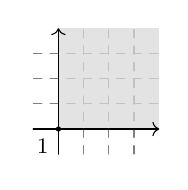
\begin{tikzpicture}        
        [line cap=round,line    join=round,x=1cm,y=1cm,baseline={0.5cm-0.5*height("$=$")}, scale=0.32]
        \draw (-0.99,-0.99)[dashed, opacity=0.5] grid (3.99,3.99);
        \fill[fill=gray!30, opacity=0.75] (0,4)--(0,0)--(4,0)--(4,4);
        \draw[->] (-1,0) -- (4,0);
        \draw [->] (0,-1) -- (0,4);
        \draw (0,0) node[below left ] {\footnotesize 1};
        \fill (0,0) circle[radius=3pt];
    \end{tikzpicture}
    = \\
    & =    
    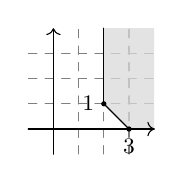
\begin{tikzpicture}        
        [line cap=round,line    join=round,x=1cm,y=1cm,baseline={0.5cm-0.5*height("$=$")}, scale=0.32]
        \draw (-0.99,-0.99)[dashed, opacity=0.5] grid (3.99,3.99);
        \fill[fill=gray!30, opacity=0.75] (2,4)--(2,1)--(3,0)--(4,0)--(4,4);
        \draw[->] (-1,0) -- (4,0);
        \draw [->] (0,-1) -- (0,4);
        \draw (2,4) -- (2,1);
        \draw (2,1)--(3,0);
        \draw (3,0)--(4,0);
        \draw (2,1) node[left] {\footnotesize 1};
        \draw (3,0) node[below]{\footnotesize 3};
        \fill (3,0) circle[radius=3pt];
        \fill (2,1) circle[radius=3pt];
    \end{tikzpicture}
    \oplus
    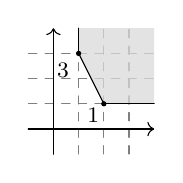
\begin{tikzpicture}        
        [line cap=round,line    join=round,x=1cm,y=1cm,baseline={0.5cm -0.5*height("$=$")}, scale=0.32]
        \draw (-0.99,-0.99)[dashed, opacity=0.5] grid (3.99,3.99);
        \fill[fill=gray!30, opacity=0.75] (1,4)--(1,3)--(2,1)--(4,1)--(4,4);
        \draw[->] (-1,0) -- (4,0);
        \draw [->] (0,-1) -- (0,4);
        \draw (1,4) -- (1,3);
        \draw (1,3)--(2,1);
        \draw (2,1)--(4,1);
        \draw (1,3) node[below left ] {\footnotesize 3};
        \draw (2.2,1.2) node[below left ] {\footnotesize 1};
        \fill (1,3) circle[radius=3pt];
        \fill (2,1) circle[radius=3pt];
    \end{tikzpicture}
    \oplus
    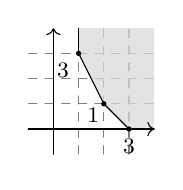
\begin{tikzpicture}        
         [line cap=round,line    join=round,x=1cm,y=1cm,baseline={0.5cm-0.5*height("$=$")}, scale=0.32]
        \draw (-0.99,-0.99)[dashed, opacity=0.5] grid (3.99,3.99);
        \fill[fill=gray!30, opacity=0.75] (1,4)--(1,3)--(2,1)--(3,0)--(4,0)--(4,4);
        \draw[->] (-1,0) -- (4,0);
        \draw [->] (0,-1) -- (0,4);
        \draw (1,4) -- (1,3);
        \draw (1,3)--(2,1);
        \draw (2,1)--(3,0);
        \draw (3,0)--(4,0);
        \draw (1,3) node[below left] { \footnotesize 3};
        \draw (2.2,1.2) node[below left]{ \footnotesize 1};
        \draw (3,0) node[below]{ \footnotesize 3};
        \fill (3,0) circle[radius=3pt];
        \fill (1,3) circle[radius=3pt];
        \fill (2,1) circle[radius=3pt];
    \end{tikzpicture}
    = \\
    & = 
    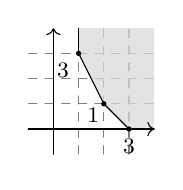
\begin{tikzpicture}        
         [line cap=round,line    join=round,x=1cm,y=1cm,baseline={0.5cm-0.5*height("$=$")}, scale=0.32]
        \draw (-0.99,-0.99)[dashed, opacity=0.5] grid (3.99,3.99);
        \fill[fill=gray!30, opacity=0.75] (1,4)--(1,3)--(2,1)--(3,0)--(4,0)--(4,4);
        \draw[->] (-1,0) -- (4,0);
        \draw [->] (0,-1) -- (0,4);
        \draw (1,4) -- (1,3);
        \draw (1,3)--(2,1);
        \draw (2,1)--(3,0);
        \draw (3,0)--(4,0);
        \draw (1,3) node[below left] { \footnotesize 3};
        \draw (2.2,1.2) node[below left]{ \footnotesize 1};
        \draw (3,0) node[below]{ \footnotesize 3};
        \fill (3,0) circle[radius=3pt];
        \fill (1,3) circle[radius=3pt];
        \fill (2,1) circle[radius=3pt];
    \end{tikzpicture}
\end{align*}
The sum above tropically vanishes, thus $S$ is a solution for $\trop_v(F)$. We now show that the initial of $F$ with respect to $(S,\omega)$ is not a monomial for every $\omega$. The vertices of $\trop_v(F)(S)$ are $V:=\{(3,0),(2,1),(1,3)\}$. Let $\omega$ with positive, rationally independent coordinates such that $(3,0) = \min_{\preceq_\omega} V$. Then we have: 
\begin{align*}
    h_{(S,\omega)} & = 2^{-3}t_1^{-3} \left ( (6t_1+\frac{5}{2}t_2 ) \cdot (2t_1x^{(0,1)})^2 + 3t_1t_2 \cdot 2t_1x^{(2,3)} + (4t_1t_2^3 + t_1^2t_2 - 4t_1^3) \cdot 2x^{(1,0)}
    \right) = \\
    & = 3+\frac{5}{4}t_2t_1^{-1}  (x^{(0,1)})^2 + \frac{3}{4}t_1^{-1}t_2 x^{(2,3)} + (t_1^{-2}t_2^3 + \frac{1}{4}t_1^{-1}t_2 - 1) x^{(1,0)}
\end{align*}
and $in_{(S, \omega)}(F)$ is the reduction of $ h_{(S,\omega)}$ modulo $\mathfrak m_{v_\omega}$:
\[
    in_{(S, \omega)}(F)= (x^{(0,1)})^2 + x^{(1,0)} \in \overline{\mathbb{F}_2}\{x\}.
\]
With analogous computations, for $\omega$ such that $(1,3) = \min_{\preceq_\omega} V$ we obtain
\[
    in_{(S, \omega)}(F)= x^{(2,3)} + x^{(1,0)},
\]
and for $\omega$ such that $(2,1) = \min_{\preceq_\omega} V$ we get 
\[
    in_{(S, \omega)}(F)= (x^{(0,1)})^2  + x^{(2,3)} + x^{(1,0)}.
\]
This reflects exactly the fact that the weighted vertices $(3,0)$ and $(1,3)$ in $\trop_v(F)(S)$ are attained twice at, respectively, the monomials $(x^{(0,1)})^2$ and $x^{(1,0)}$, and $x^{(2,3)}$ and $x^{(1,0)}$, while $(2,1)$ is attained three times, at all the monomials in the support of $F$.
\end{ex}

\section{Differential Berkovich analytification and the fundamental theorem} \label{sec:berkovich}

In this section we complete the proof of Theorem \ref{theorem:fundamental-introduction} by proving a differential version of the statement of \cite[Theorem 4.2]{draisma} and 
\cite[Proposition 2.2]{payneanal}. Before proving this result, we will recall the definition of the differential tropicalization functor and of differential Berkovich space. 

Given a differential ring $(R,\{d_{R,i}\}_{i \in [m]})$ let $\mathbf v = (v, \widetilde v) \co R \rightarrow \mathbf S =(S_1 \rightarrow S_0)$ be a differentially enhanced valuation to a reduced pair $\mathbf S$. Let $A$ be a finitely generated differential algebra over $R$, i.e.\ $A \cong R\{z_1, \dots , z_q\} /I$ for some integer $q$ and differential ideal $I$.
\begin{defin}
Given an $\mathbf {S}$-algebra $\mathbf{T} =(T_1 \rightarrow T_0)$, a differentially enhanced valuation $\mathbf{w}=(\widetilde{w}, w) \co A \rightarrow \mathbf T$ is said to be compatible with $\mathbf{v}$ if the diagram
	\begin{equation} \label{diagr:comp-diff-enh}
		\begin{tikzcd}
		& S_1 \arrow[r] \arrow[dd] & T_1 \arrow[dd] \\
		A \arrow[rrd, crossing over, near end, "w"] \arrow[rd, "v"'] \arrow[ru, "\widetilde{v}"] \arrow[rru, crossing over, "\widetilde{w}"', near end] 
		&                          &                \\
		& S_0 \arrow[r]            & T_0           
		\end{tikzcd}
	\end{equation}
commutes.
\end{defin}
\begin{defin}
Given an $\mathbf{S}$-algebra $\mathbf{T}$, the \emph{differential Berkovich space over $\mathbf{T}$} of $A$ is the set $\mathit{Berk}_{\mathbf{T}}(A)$ of differentially enhanced valuations $\mathbf{w}:=(w, \widetilde w) \co A \to \mathbf{T}$ that are compatible with $\mathbf{v}$.
\end{defin}

\begin{defin}
     A \emph{differential presentation} of $A$ is a surjective morphism of differential algebras over $R$ of the form $\varphi \co \diff R n \twoheadrightarrow A$ for some $n$. 
     
     The category of affine differential presentations $\mathbf{Pres}_{A}^\text{d}$ is the category whose objects are differential presentations of $A$, and whose morphisms between the objects $\varphi \co \diff R n \twoheadrightarrow A$ and $\psi:R\{y_1,\dots,y_m\}\twoheadrightarrow A$ are morphisms of differential algebras which make the following diagram commute:
     \begin{center}
    \begin{tikzcd}
    R\{x_1, \dots , x_n\} \arrow[dr, swap, twoheadrightarrow, "\varphi"] \arrow[rr]&  & R\{y_1, \dots , y_m\} \arrow[dl, twoheadrightarrow, "\psi"]\\
    &A&
    \end{tikzcd}
    \end{center}
     
     Finally, denote by $\mathbf{Pres}_{A}^\text{d, lin}$ the subcategory of presentations with linear morphisms (see \cite[Section 5.3]{gianmereta} for details).
 \end{defin}   

 \begin{defin}\cite[Definition 5.1.1]{eqtrop}
    Let $S$ be an idempotent semiring and $M$ a monoid. Given $f = \sum_{\jj} s_\jj x^\jj \in S[M]$, the \emph{bend congruence} of $f$ is the semiring congruence on $S[M]$ generated by the following set of relations, called the \emph{bend relations} of $f$:
    \[
        \left \{ \sum_{\jj} s_\jj x^\jj  \sim \sum_{\jj \neq \hh} s_\jj x^\jj  \right \} _{\hh \in \textit{supp}(f)}.
    \]
    We will denote this congruence as $\bend(f)$. For an ideal $I$ of  $S[M]$, we will denote by $\bend(I)$ the congruence generated by the bend relations of all elements of $I$.
\end{defin}
Notice that for $M = \N^m$, we have $S[M]=\basic S n $.
Given a differential presentation $\varphi \co \diff R n \twoheadrightarrow A$ of $A$, let $I := \ke \varphi$. It is a differential ideal, thus $\trop_v(I)$ is an ideal of $\basic S n$. Consider the extension of the bend congruence $\bend(\trop_v(I))$ to $ (S_0|S_1)\{x_1, \dots , x_n\}$, denoted again $\bend(\trop_v(I))$. Writing $\diff {\mathbf S} n /\!/ \bend(\trop_v(I))$ for the reduction of the pair 
\[
    \diff {S_1} n \rightarrow  (S_0|S_1)\{x_1, \dots , x_n\}/\bend(\trop_v(I)),
\]
the assignment 
 \[
    \varphi \mapsto \diff {\mathbf S} n /\!/ \bend(\trop_v(I))
 \]
is a functor $\Trop^d \co \mathbf{Pres}_{A}^\text{d} \rightarrow \alg{\mathbf S}$.

For any integer $m$, in a similar fashion as for the non-differential case it is possible to define a universal differential presentation of $A$ and obtain a differential version of Payne's inverse limit theorem and of \cite[Theorem 4.4.1]{univtrop}:
\begin{prop}(\cite[Corollary 5.5.1]{gianmereta}\cite[Section 8]{tesimereta})\label{isomorphisms}
Denoting by $\DTrop_\textit{univ}(A)$ the tropicalization of the universal differential presentation of $A$, we obtain: 
\[
    \DTrop_\textit{univ}(A)
    \cong \colim_{ \mathbf{Pres}_A^\textup{d,lin}} \DTrop.
\] 
Furthermore, for any $\mathbf S$-algebra $\mathbf T$: 
\[
    \textup{Hom}_{\alg {\mathbf S}}(\DTrop_\textit{univ}(A), \mathbf T) \cong \mathit{Berk}_{\mathbf{T}}(A).
\]
\end{prop}
Given an $\mathbf S$-algebra $\mathbf{T}$, the set $\textup{Hom}_{\alg {\mathbf S}}(\DTrop(\varphi), \mathbf T)$ is the set of tropical solutions to $A$ in $\mathbf T$, with respect to the presentation $\varphi$ (i.e.\ the tropical solutions in $\mathbf T$ of $\trop_v(\ke \varphi)$). By \cite[Proposition 4.4.1]{gianmereta}, $\textup{Hom}_{\alg {\mathbf S}}(\DTrop(\varphi), \mathbf T)$ can be identified with the set of tuples $(y_1, \dots , y_n) \in T_1^n$ such that the elements $\pi(d^jy_i) \in T_0$ define an $S_0$-algebra morphism 
\[
    \basic {S_0} n / \bend(\trop_v(I)) \rightarrow T_0.
\]
In this setting, we have the following differential version of \cite[Theorem 4.2]{draisma},
\cite[Proposition 2.2]{payneanal}:

    \begin{teorema}
    For any differential presentation $\varphi$ of the differential algebra $A$, under the identification of $\textup{Hom}_{\alg {\mathbf S}}(\DTrop(\varphi), \mathbf T)$ with a subset of $T_1^n$ described above, the following equality holds:
    \begin{equation} \label{eq:4th-fund}
        \textup{Hom}_{\alg {\mathbf S}}(\DTrop(\varphi), \mathbf T) = \{(\widetilde w (\varphi(x_1)), \dots , \widetilde w (\varphi(x_n))) \in T_1^n \mid (w, \widetilde w) \in \mathit{Berk}_{\mathbf{T}}(A) \}.
    \end{equation}
Moreover, when $\mathbf T = \mathbf \Gamma_m$, equation \ref{eq:4th-fund} gives the equality of point (2) and point (4) of Theorem \ref{theorem:fundamental-introduction}. 
\end{teorema}
\begin{proof}
It follows from the isomorphisms in Proposition \ref{isomorphisms} that 
 \[
    \mathit{Berk}_{\mathbf{T}}(A) \cong 
    \lim_{ \mathbf{Pres}_A^\textup{d,lin}} \textup{Hom}_{\alg {\mathbf S}}(\DTrop(-),\mathbf T).
    \]
    Hence, it suffices to show that given a differential presentation $\varphi$ and an element $(w,\widetilde w)$ in $\mathit{Berk}_{\mathbf{T}}(A)$, the tuple $(\widetilde w (\varphi(x_1)), \dots , \widetilde w (\varphi(x_n)))$ corresponds to an element of $\textup{Hom}_{\alg {\mathbf S}}(\DTrop(\varphi), \mathbf T)$; that is, that there is a well-defined morphism of $S_0$-algebras 
    \[
    \beta_{\varphi, \widetilde w} \co \basic {S_0} n/\bend(\trop_v(I))  \rightarrow T_0
    \]
    where $I=\ker(\varphi)$, given by sending (the congruence class of) each $x_i^{(\jj)}$ to $\pi(d_{T_1}^\jj\widetilde w(\varphi(x_i)))$. Clearly, this amounts to showing that for every $f \in I$ we have that $\beta_{\varphi, \widetilde w}(f)$ tropically vanishes.
    
    For every $i,\jj$, we have the following equalities: 
    \[
         \pi(d_{T_1}^\jj\widetilde w(\varphi(x_i))) =  \pi(\widetilde w (d_A^\jj \varphi(x_i))) 
         = w (d_A^\jj \varphi(x_i)) = w (\varphi (x^{(\jj)}_i)).
    \]
    Given $f \in I$, write it as $\sum_\Lambda a_\lambda \prod_{i,\jj}(x_i^{(\jj)})^{\lambda_{i,\jj}}$. By definition of $I$, we have
    \[
    0 = \varphi(f) = \sum_\Lambda a_\lambda \prod_{i,\jj}(\varphi(x_i^{(\jj)}))^{\lambda_{i,\jj}} \in A.
    \]
    Thus, the sum $\sum_\Lambda v(a_\lambda) \prod_{i,\jj} w(\varphi(x_i^{(\jj)}))^{\lambda_{i,\jj}}$ tropically vanishes in $T_0$, as we wanted.
\end{proof}

\color{black}

\section{The radius of convergence of solutions to a nonarchimedean differential equation}\label{section:raggi}

In this section we focus on the case $m=1$ and introduce a notion of radius of convergence for elements of $\pt$. Then, given a nontrivially valued field
$K$, we state a corollary of Theorem \ref{theorem:fundamental} relating this tropical notion of radius of convergence to the classical one for solutions of a differential equation over $\pk$.

\begin{defin}\label{definition:conv-radius}
    Given $A = \sum_{i=0}^\infty a_i t^i \in \pt$, we define its radius of convergence with respect to the real number $c > 1$ as:
    \[
        r_c(A):= \sup \{r \in [0,\infty) \mid \lim_{i \to +\infty} c^{-a_i} r^i = 0\} \in [0,\infty]
    \]
    with the convention that $c^{- \infty} = 0$ for any $c > 1$.
\end{defin}

\begin{oss}
    Notice that choosing any other real number $c'$ in the definition above gives the following relation between the radii of convergence of a tropical power series $A$:
    \[
        r_c(A) = r_{c'}(A) ^{\frac{1}{\log_c(c')}}.
    \]
\end{oss}
Let us consider now a field $K$ equipped with a nontrivial valuation $v_K \co K \rightarrow \T$, and assume the valuation $v$ has a section. For every $x \in K$, the norm on $K$ associated to $v_K$ is defined as $|x|_{K}:=c ^{-v_K(x)}$ for some $c > 1$. Canonical choices for $c$ are $c:=p$ when $v$ is the $p$-adic valuation for some prime number $p$ and $c:=e$ when $v$ is the $t$-adic valuation. 

Given a power series $A = \sum_{i=0}^\infty a_i t^i  \in \pk$ its radius of convergence is defined as follows: 
\[
        r(A):= \sup \{r \in [0,\infty) \mid \lim_{i \to +\infty} |a_i|_{K} r^i = 0\} \in [0,\infty].
\]
It is clear that, endowing $\pk$ with the differentially enhanced valuation $\mathbf{v}$, for every $A \in \pk$ we have the equality:
\[
    r(A) = r_{c}(\trop_{\widetilde v}(A)).
\]
where $c$ is chosen to be the same as in the definition of $| \! -  \! |_{K}$. 
Thus the following corollary of the Fundamental Theorem follows directly:

\begin{cor}
    Let $I \in \pk\{x\}$. Then:
    \[
        \{r(A) \mid A \in \textup{Sol}_{\pk}(I)\} = \{r_{c}(S)  \mid S \in \textup{Sol}_{\mathbf{S}}(\trop_v(I))\}.
    \]
\end{cor}
We give here an example of computation of the solutions of the tropicalization of a linear $p$-adic differential equation.
\begin{ex}\label{ex:p-adic-diffeq}
Let $p$ a prime number and consider the differential enhancement $\mathbf v$ as above for $K=\C_p$ endowed with the $p$-adic valuation. Let $\zeta \in \C_p$ such that $\zeta^{p-1} = -p$, and consider the equation $f = x' - p \zeta t^{p-1} x  \in \C_p[\![t]\!]\{x\}$. $p$-adic solutions at the origin to this equations are $p$-adic multiples of $\exp( \zeta t^p) = \sum_{n =0}^\infty (1/n!) (\zeta t^p)^n \in \C_p[\![t]\!]$. The interest of this $p$-adic differential equation lies in the fact that it is somehow the easiest example for which we can observe the piecewise linear behaviour of the radius of convergence as a function of the distance of the expansion point from the origin. In particular, $\exp( \zeta t^p)$ has radius of convergence 1 but there exists an $r > 1$ such that for solutions at $|x|_p > r$ the radius of convergence decreases. Let us see a concrete example of a computation of the solutions to a linear tropical differential equation, by computing the set of solutions to the tropicalization of the generators (as an ideal) of the differential ideal generated by $f$. 

One can prove by induction that $n$-th derivative of $f$ can be expressed as: 
\begin{equation*}
d^n f =
\begin{cases*}
x^{(n+1)} - \sum_{i=0}^n  \binom{n}{i} \zeta \prod_{k=0}^{n-i} (p-k) t^{p-1-n+i} x^{(i)} & if $n < p$ \\
x^{(n+1)} - \sum_{i=0}^{p-1} \binom{n}{p-1-i} \zeta \prod_{k=0}^{p-1-i} (p-k) t^{p-1-i} x^{(i+n-p+1)}  & if $n \ge p$
\end{cases*}
\end{equation*}
which implies: 
\begin{equation*}
\trop_v(d^n f ) =
\begin{cases*}
x^{(n+1)} + \sum_{i=0}^n (p-1-n+i, v_p( \binom{n}{i}) + \frac{p}{p-1})  x^{(i)}& if $n < p$ \\
x^{(n+1)} + \sum_{i=0}^{p-1}  (i, v_p( \binom{n}{p-1-i}) + \frac{p}{p-1})  x^{(i+n-p+1)}    & if $n \ge p$
\end{cases*}
\end{equation*}
We prove that a solution $S= \sum_{k=0}^\infty s_k t^k$ to the tropical system $\{\trop_v(d^n f)\}_{n \in N}$ is of the form $c \odot A$, where $c \in \T$ and $A = \sum_{k=0}^\infty a_k t^k \in \pt_{v_p}$ for:
\begin{equation*}
a_k =
\begin{cases*}
\infty & if $p \ndiv k$ \\
\frac{m}{p-1} - v_p(m!)  & if $k = mp$
\end{cases*}
\end{equation*}
i.e.\ that $A$ is the tropicalization of $\exp (\zeta t^p)$ and the set of solutions to $\trop_v(I)$ is a tropical linear space as expected. We prove this by induction on $k$. For $k=0$ this is trivially satisfied as $p \mid 0$ and $0 = \frac{0}{p-1} - v_p(0!)$. For $0 < k \le p$, consider $\textup{trop}(f) = x' + (p-1, \frac{p}{p-1})x$ and 
\[
\textup{trop}_v(f)(A) = (0, a_1) \oplus \left (p-1, \frac{p}{p-1} \right) .
\]
As $A$ a solution, $a_k$ has to be equal to $\infty$ for every $0 < k < p$, thus we obtain: 
\[
\textup{trop}_v(f)(A) = (p-1, a_p +1) \oplus \left ( p-1, \frac{p}{p-1} \right )
\]
which gives $a_p = \frac{1}{p-1} = \frac{1}{p-1} - v_p(1!) $.


In general, let  $Mp < k \le (M+1)p$ for some $M \in \N$ and assume the inductive hypothesis holds for $Mp$. Notice that $v_p \left ( \binom{Mp}{p-1-i} \right )= 1$ for all $M \in \N$ and for all $i \in \{0, \dots , p-2\}$, thus:
\[
\trop_v(d^{Mp}f) = x^{(Mp+1)} + \left ( p-1, \frac{p}{p-1} \right ) x^{(Mp)} +  \sum_{j=1}^{p-1}  \left ( p-1-j, \frac{p}{p-1} +1 \right )  x^{(Mp- j)}
\] 
where $j:=i-p+1$.  We obtain that $\trop_v(d^{Mp}f) (A)$ is equal to:
\begin{equation*}
\begin{split}
& \left ( 0, a_{Mp+1} + \sum_{m=1}^M v_p(mp) \right ) \oplus   \left ( p-1, \frac{p}{p-1} \right ) \odot \left  ( 0, \frac{M}{p-1} - v_p(M!) +  \sum_{m=1}^M v_p(mp) \right )  \oplus \\
&  \bigoplus_{j=1}^{p-1}  \left ( p-1-j, \frac{p}{p-1} +1 \right ) \odot \left (j  ,   \frac{M}{p-1} - v_p(M!) + \sum_{m=1}^{M} v_p(mp)  \right )\\
\end{split}
\end{equation*}
As the first coordinate of every addendum of the sum above, except for the first one, is equal to $p-1$ and $A$ is a solution, we have as before that $a_k$ has to be equal to $\infty$ for $Mp < k < (M+1)p$. For $k=(M+1)p$, since the following holds:
\[
\sum_{m=1}^M v_p(mp) = \sum_{m=1}^M ( 1+ v_p(m) ) = M + v_p(M!)
\]
we have:
\begin{equation*}
\begin{split}
\trop_v(d^{Mp}f) (A) = & \left ( p-1, a_{(M+1)p} + M+1 +v_p((M+1)!) \right ) \oplus    \left  ( p-1 , \frac{M +p}{p-1} + M  \right )  \oplus \\
&  \oplus \left ( p-1 , \frac{M +p}{p-1}   + M +1 \right )\\
\end{split}
\end{equation*}
which gives:
\[
a_{(M+1)p} +1 +v_p((M+1)!) = \frac{M +p}{p-1} .
\]
The last equality implies $a_{(M+1)p}= \frac{M +1}{p-1} - v_p((M+1)!)$. Lastly, it is easy to check that every tropical multiple of $A$ is again a solution to the tropical system $\{\trop_v(d^n f)\}_{n \in N}$, as these are linear equations.
\end{ex}
    \begin{oss}
    Notice that in Example \ref{ex:p-adic-diffeq} above we also proved that $\{f\} \subset I$ is a \emph{tropical differential basis} for $I$, in the sense of \cite[Definition 4.1]{FT20}, i.e. a set $G \subset I$ such that 
    \[
        \textup{Sol}_{\mathbf{S}}(\trop_v(I)) = \bigcap_{g \in G} \bigcap_{k \in \N}\textup{Sol}_{\mathbf{S}}(\trop_v(d^k g)).
    \]
    In the same paper the authors, working in Grigoriev's setting, give an example of a differential ideal $I$ generated by linear forms that does not admit a finite tropical differential basis of linear forms, in contrast with the behaviour of tropical basis in the non-differential setting (see \cite[Theorem 2.6.6]{macsturm}).
    \end{oss}
    This work moves the first steps towards the development of methods using tropical techniques to compute the radius of convergence function, without a priori knowing the solutions to the differential equation. To this aim, it is necessary to introduce a notion of tropical differential basis satisfying a finiteness condition as in the classical case, or at least find criteria for finiteness of basis as above to hold and methods to identify such collections. This, at least in the linear case, would make similar computation as above possible, without knowing how the solutions over $\pk$ look like.
    Furthermore, the methods we explained here are only useful to compute single values of the radius of convergence function so far, thus a way to tropically move the point of expansion has to be developed in order to capture the global behaviour of this function.
    The authors intends to pursue both these direction of research in the near future.


\section*{Table of notations}
If not specified otherwise, the following notations will have the following meaning:
\begin{center}
\begin{longtable}{p{3cm} p{12cm}}
$m$ & a positive integer \\
$[m]$ & the set $\{1, \dots , m\}$\\
$e_i$ & the $i$-th standard basis vector of $\R^m$ \\
$\langle \cdot, \cdot \rangle $ & the scalar product of two vectors of $\R^m$ \\
$\tau, \rho$ & a strongly convex, rational polyhedral cone of dimension $m$ in $\R^m$\\
$C_\tau(Z)$ &the convex hull with respect to $\tau$ of a subset $\Z \subseteq \R^m$  \\
$\textup{Vert}_\tau(Z)$ & the set of vertices of $C_\tau(Z)$\\
$\B$ & the idempotent semiring $(\{0, \infty\}, \min, +)$\\
$\T$ & the idempotent semiring $(\R\cup \{\infty\}, \min, +)$\\
$\T_m$ & the idempotent semiring $(\R^m\cup \{\infty\}, \min_{\text{lex}}, +)$ \\
$\widetilde{G}$ & the idempotent semiring $(G \cup \{\infty\}, \min_\preceq, +)$ for a totally ordered monoid $(G,+, \preceq)$\\
$\omega$ & a vector of $(\R_{>0})^m$ with rationally independent coordinates\\
$H_\omega$ & the halfspace $\{x \in \R^m \mid \langle x, \omega \rangle \ge 0 \}$\\
$\textup{Lead}_\omega(G, S)$ & the idempotent semiring of leading terms with respect to $\omega$ of an additive submonoid $G \subseteq \Q^m$, weighted in $S$\\
$\textup{Conv}(\tau,S)$ &  the idempotent semiring of convex hulls w.r.t.\ $\tau$ with vertices weighted in an idempotent semiring $S$ \\
$\textup{Conv}_m(S)$ &  the idempotent semiring $\textup{Conv}(\tau,S)$ for $\tau = (\R_{\ge 0})^m$ \\
$\textup{Conv}(\tau,S)_{\{e_i\}}$ & the localization of $\textup{Conv}(\tau,S)$ in the translates of $\tau$\\
$\sigma_0$ & the support map $\textup{Conv}(\tau,S) \rightarrow \textup{Conv}(\tau,\B)$ of Remark \ref{oss:Conv-m=1} \\
$K$ & an uncountable algebraically closed field of characteristic 0 \\
$v_\text{triv}$ & the trivial valuation $K \rightarrow \B$\\
$v_K$ & a nontrivial valuation $K \rightarrow \T$\\
$R_K$ & the valuation ring of $v_K$ \\
$\mathfrak m_K$ & the maximal ideal of $R_K$ \\
$k$ & the residue field $R_K / \mathfrak m _K$ of $v_K$ \\
$\pi_K$ & a uniformizer of $v_K$ \\
$\Gamma_K$ & the value group of $v_K$ \\
$R_\nu$ & the valuation ring of a valuation $\nu$ \\
$\mathfrak m_\nu$ & the maximal ideal of $R_v$, for a valuation $\nu$\\
$\supp(A)$ & the support of the power series A\\
$\pkcone \tau$ & the ring of power series over $K$ with support in $ \Z^m \cap \tau$\\
$\pkk m$ & the ring $\pkcone \tau$ for $\tau = (\R_{\ge 0})^m$\\
$\pkcone \tau _{t_1, \dots, t_m}$ & the localization of $\pkcone \tau$ in the variables\\
$K(\!(t_1, \dots , t_m)\!)_\omega$ & the field of multivariate Laurent series with support contained in a translate of $H_\omega$ \\
$R_m$ & the ring $\pkk m$\\
$w_\tau$ & the valuation $\pkcone \tau \rightarrow \textup{Conv}(\tau, \B)$ of point (1) of Example \ref{ex:conv-vals} \\
$v_\tau$ & the valuation $\pkcone \tau \rightarrow \textup{Conv}(\tau, \T)$ of point (2) of Example \ref{ex:conv-vals} \\
$v_\omega$ & the valuation $K(\!(t_1, \dots , t_m)\!)_\omega \rightarrow \textup{Lead}_\omega(\Z^m, \T)$ as in \ref{eq:v-omega} \\
$w$ & the valuation $w_\tau$ for $\tau = (\R_{\ge0})^m$ \\
$v$ & the valuation $v_\tau$ for $\tau = (\R_{\ge0})^m$ \\
$\pb$ & the strict differential semiring of Boolean power series \\
$\pt_v$ &  the (non-strict) differential semiring of tropical power series, with differential w.r.t.\ a nontrivial valuation $v \co \N \rightarrow \T$  \\
$\pbb m$ &  the strict partial differential semiring of multivariate Boolean power series \\
$\ptt n _v$ &  the (non-strict) partial differential semiring of multivariate tropical power series, with differentials w.r.t.\ a nontrivial valuation $v \co \N \rightarrow \T$\\
$\diff R n$ & the differential algebra of differential polynomials in $n$ variables over a differential ring $R$ as in \cite{ritt} \\
$\diff S n$ & the differential algebra of differential polynomials in $n$ variables over a differential semiring $S$ as in \cite{gianmereta} \\
$\basic S n$ & the $S$-algebra $S[x_i^{(\jj)} \mid i \in [n], \jj \in \N^m]$ over a differential semiring $S$ with $m$ differentials \\
$\diff{(S_1|S_0)}{n}$ &  the pushout of Diagram \ref{eq:pushout-diagram}, for a (partial) tropical pair $S_1 \rightarrow S_0$\\
$\diff{\mathbf S} n$ & the $\mathbf S$-algebra of differential polynomials in $n$ variables over a (partial) tropical pair $\mathbf S$, as in Definition \ref{def:diff-poly-over-pair}\\
$\mathbf T _m$ & the (partial) tropical pair $\Psi_m \co \pbb m \to \textup{Conv}_m(\B)$ of point (3) of Example \ref{ex:pairs} \\
$\mathbf T$ & the tropical pair $\mathbf T _m$ for $m=1$, i.e.\  $\Psi \co \pb  \to \T$ \\
$\mathbf S _m$ & the (partial) tropical pair $\Phi_m \co {\ptt m}_v \to \textup{Conv}_m(\T)$ of point (4) of Example \ref{ex:pairs} \\
$\mathbf S$ & the tropical pair $\mathbf S _m$ for $m=1$, i.e.\ $\Phi \co \pt_v  \to \T_2$  \\
$\mathbf \Gamma _m$ & the (partial) tropical pair obtained from $\mathbf S _m$ restricting coefficients and weights to $\Gamma_K$, as in Remark \ref{oss:restr-of-diff-enh} \\
$\sigma$ & the morphism of pairs $(\sigma_0, \sigma_1 ) \co \mathbf S _m \rightarrow \mathbf T _m$, as in Diagram \ref{diagram:refined-to-grig}\\
$\widetilde w$ & submultiplicative seminorm $\pkk m \rightarrow \pbb m$ given by coefficientwise trivial valuation, as in point (3) of Example \ref{ex:diff-enhancements} \\
$\widetilde v$ & submultiplicative seminorm $\pkk m \rightarrow {\ptt m}_v$ given by coefficientwise application of a valuation $v$, as in point (4) of Example \ref{ex:diff-enhancements} \\
$\mathbf w$ & the differentially enhanced valuation $(w, \widetilde w) \co \pkk m \rightarrow \mathbf T _m$ of point (3) of Example \ref{ex:diff-enhancements}, used in \cite{grig, aroca, sebastian, FT20} \\
$\mathbf v$ & the differentially enhanced valuation $(v, \widetilde v)  \co \pkk m \rightarrow \mathbf S _m$ of point (4) of Example \ref{ex:diff-enhancements}, introduced in \cite{gianmereta, tesimereta} 
\end{longtable}
\end{center}






\begin{comment}
In the following table we make a recap of the differential enhancements that we use the most in the present work.
\begin{center}
\begin{tabular}{|p{3.5cm}||p{4.5cm}|p{6.5cm}|}
 \hline
 \multicolumn{3}{|c|}{Differential enhancements} \\
 \hline\hline
 & ODEs: $m=1$ & PDEs: $m \ge 2$ 
 \\ \hline
 \multirow{4}{3.5cm}{Trivial valuation $v_\triv \co K \rightarrow \B$} 
 &
\begin{tikzcd}
& \pb \arrow[d, "\Psi"] \\
\pk \arrow[ur, "\widetilde{w}"] \arrow[r, swap, "w"] & \mathbb{T} 
\end{tikzcd} 
& 
\begin{tikzcd}
		&\pbb m\arrow[d, "\Psi_m"] \\
		\pkk m \arrow[ur, "\widetilde{w}"] \arrow[r,swap,"w"] &  \textup{Conv}_m(\B)
\end{tikzcd} 
\\ 
  \cline{2-3}
& $w \co \sum_{}$ & cell6 \\ 
\cline{2-3}
& cell8 & cell9 \\
\cline{2-3}
& cell8 & cell9 \\
 \hline
 \multirow{3}{3.5cm}{Nontrivial valuation $v_K \co K \rightarrow \T$} 
 &
    \begin{tikzcd}
        & \pt_{v_K} \arrow[d,"\Phi"] \\
        \pk \arrow[ur, "\widetilde{w}"] \arrow[r, swap, "w"] & \T_2 
    \end{tikzcd} 
& 
    \begin{tikzcd}
        &\ptt m _{v_K} \arrow[d, "\Psi_m"] \\
        \pkk m \arrow[ur, "\widetilde{w}"] \arrow[r,swap, "w"] &  \textup{Conv}_m(\T)
    \end{tikzcd} 

\\   \cline{2-3}
& cell5 & cell6 \\
\cline{2-3}
& cell8 & cell9 \\
\cline{2-3}
& cell8 & cell9 \\
 \hline
\end{tabular}
\end{center}
\end{comment}









\newcommand{\etalchar}[1]{$^{#1}$}
	\begin{thebibliography}{CCRH{\etalchar{+}}21}

        \bibitem[ACJ03]{arocacanojung}  Fuensanta Aroca, José Cano, and Françoise Jung. \newblock{Power series solutions for non-linear PDE's}, \newblock{ \em Proceedings of the 2003 international symposium on Symbolic and algebraic computation}. 2003.
  
	\bibitem[AGT16]{aroca}
	Fuensanta Aroca, Cristhian Garay, and Zeinab Toghani.
		\newblock {The fundamental theorem of tropical differential algebraic
			geometry}.
		\newblock {\em{Pacific Journal of Mathematics}}, 283(2):257--270, 2016.
	
        \bibitem[AR19]{arocarond}
        Fuensanta Aroca and Guillaume Rond. \newblock{Support of Laurent series algebraic over the field of formal power series}. \newblock{\em Proceedings of the London Mathematical Society} 118.3 (2019): 577-605.
 
		\bibitem[Bal10]{baldassarri2010continuity}
		Francesco Baldassarri.
		\newblock Continuity of the radius of convergence of differential equations on
		p-adic analytic curves.
		\newblock {\em Inventiones mathematicae}, 182(3):513--584, 2010.
		
		\bibitem[BB19]{Baker-Bowler}
		Matthew Baker and Nathan Bowler.
		\newblock Matroids over partial hyperstructures.
		\newblock {\em Adv. Math.}, 343:821--863, 2019.

		\bibitem[BdV07]{baldassarri2007continuity}
		Francesco Baldassarri and Lucia di~Vizio.
		\newblock Continuity of the radius of convergence of p-adic differential
		equations on Berkovich analytic spaces.
		\newblock {\em arXiv preprint arXiv:0709.2008}, 2007.
		
		
		\bibitem[Ber90]{ber}
		Vladimir~G. Berkovich.
		\newblock {Spectral theory and analytic geometry over non-Archimedean
			fields}.
		\newblock American Mathematical Soc., 1990.
        
		\bibitem[Bou04]{bourbaki}
		Nicolas Bourbaki.
		\newblock Theory of sets.
		\newblock In {\em Theory of Sets}, pages 65--129. Springer, 2004.

         
		\bibitem[BFG{\etalchar{+}}23]{initialslara}
		Lara Bossinger, Sebastian Falkensteiner,
        Cristhian Garay, and Marc Paul Noordman,  .
		\newblock Tropical initial degeneration for systems of algebraic differential equations.
		\newblock {\em{arXiv:2309.10761}}, 2023.
  
        \bibitem[BFN{\etalchar{+}}21]{bouliermodel}
		Fran{\c{c}}ois Boulier, Sebastian Falkensteiner, Marc Paul Noordman,  and Omar Le{\'o}n S{\'a}nchez.
		\newblock On The Relationship Between Differential Algebra and Tropical Differential Algebraic Geometry.
		\newblock {\em{Computer Algebra in Scientific Computing: 23rd International Workshop}}, CASC 2021, Sochi, Russia, September 13--17, 2021, Proceedings 23, 62--77, Springer, 2021.

        \bibitem[Chr11]{christol2011radius}
		Gilles Christol.
		\newblock The radius of convergence function for first order differential
		equations.
		\newblock {\em Advances in non-Archimedean analysis}, 551:71--89, 2011.
        \bibitem[CCRH{\etalchar{+}}21]{YaironMac}
		Justin Chen, Yairon Cid-Ruiz, Marc H{\"a}rk{\"o}nen, Robert Krone, and Anton
		Leykin.
		\newblock Noetherian operators in macaulay2.
		\newblock {\em arXiv preprint arXiv:2101.01002}, 2021.
  
		\bibitem[CD94]{christol1994modules}
		Gilles Christol and Bernard Dwork.
		\newblock Modules diff{\'e}rentiels sur les couronnes.
		\newblock In {\em Annales de l'institut Fourier}, volume~44, pages 663--701,
		1994.
		
		\bibitem[CGL20]{cotterill}
		Ethan Cotterill, Cristhian Garay, and Johana Luviano.
		\newblock Exploring tropical differential equations.
		\newblock {\em{arXiv:2012.14067}}, 2020.
		
		\bibitem[CGM20]{Noah-module-theoretic}
		Colin {Crowley}, Noah {Giansiracusa}, and Joshua {Mundinger}.
		\newblock {A module-theoretic approach to matroids}.
		\newblock {\em {J. Pure Appl. Algebra}}, 224(2):894--916, 2020.
		

        \bibitem[CP16]{charles2016bertini}
        Fran\c{c}ois Charles and Bjorn Poonen.
        \newblock Bertini irreducibility theorems over finite fields.
        \newblock {\em J. Amer. Math. Soc.}, 29:81--94, 2016.
		
		\bibitem[CR94]{librorobba}
		Gilles Christol and Philippe Robba.
		Equations différentielles p-adiques.
		\newblock Hermann, 1994.


        \bibitem[Dra08]{draisma}
		Jan Draisma.
		A tropical approach to secant dimensions.
		\newblock {\em {J. Pure Appl. Algebra}}, 212(2):349--363, 2008.
  
		\bibitem[DGS16]{librodwork}
		Bernard Dwork, Giovanni Gerotto, and Francis~J Sullivan.
		An Introduction to G-Functions.(AM-133), Volume 133, volume
		133.
		\newblock Princeton University Press, 2016.
		
		\bibitem[EKL06]{kapranov}
		Manfred Einsiedler, Mikhail Kapranov, and Douglas Lind.
		\newblock Non-archimedean amoebas and tropical varieties.
		\newblock {\em J. Reine Angew. Math.}, 2006.
		
		\bibitem[EMHS22]{ridamarc}
		Rida~Ait El~Manssour, Marc H{\"a}rk{\"o}nen, and Bernd Sturmfels.
		\newblock Linear pde with constant coefficients.
		\newblock {\em Glasgow Mathematical Journal}, pages 1--26, 2022.
		
		\bibitem[FGH{\etalchar{+}}20]{sebastian}
		Sebastian {Falkensteiner}, Cristhian {Garay}, Mercedes {Haiech}, Marc~Paul
		{Noordman}, Zeinab {Toghani}, and Fran\c{c}ois {Boulier}.
		\newblock {The fundamental theorem of tropical partial differential algebraic
			geometry}.
		\newblock In {\em {Proceedings of the 45th international symposium on symbolic
				and algebraic computation, ISSAC '20, Kalamata, Greece, July 20--23, 2020}},
		pages 178--185. ACM, 2020.

            \bibitem[FM23]{sebastianmereta} 
            Sebastian Falkensteiner and Stefano Mereta. \newblock \emph{The fundamental theorem of tropical differential algebra for formal Puiseux series},
            \newblock preprint at \emph{https://www.researchsquare.com/article/rs-3256404/v1}
            
		
	\bibitem[FT20]{FT20}
	Alex Fink and Zeinab Toghani,              Initial forms and a notion        of basis for
		tropical differential equations, \emph{Pacific Journal of Mathematics} 318.2 (2022): 453-468.

  
		\bibitem[GG16]{eqtrop}
		Jeffrey Giansiracusa and Noah Giansiracusa.
		\newblock Equations of tropical varieties.
		\newblock {\em Duke Mathematical Journal}, 165(18):3379--3433, 2016.

  
		\bibitem[GG18]{GG3}
		Jeffrey Giansiracusa and Noah Giansiracusa.
		\newblock A {G}rassmann algebra for matroids.
		\newblock {\em Manuscripta Mathematica}, 156(1-2):187--213, 2018.


        \bibitem[GG22]{univtrop}
		Jeffrey Giansiracusa and Noah Giansiracusa.
		\newblock The universal tropicalization and the Berkovich analytification.
		\newblock {\em {Kybernetika}}, vol. 58, number 5, 790-815, 2022.

  
		\bibitem[GM23]{gianmereta}
		Jeffrey Giansiracusa and Stefano Mereta.
		\newblock A general framework for tropical differential equations.
		\newblock {\em Manuscripta Mathematica, https://doi.org/10.1007/s00229-023-01492-5}, 2023.
		
		\bibitem[Gol13]{golan}
		Jonathan~S Golan.
		Semirings and their Applications.
		\newblock Springer Science \& Business Media, 2013.
		
		\bibitem[{Gri}17]{grig}
		Dima {Grigoriev}.
		\newblock {Tropical differential equations}.
		\newblock {\em {Adv. Appl. Math.}}, 82:120--128, 2017.
		
		\bibitem[Gr{\"o}10]{grobmac}
		Wolfgang Gr{\"o}bner.
		\newblock On the Macaulay inverse system and its importance for the theory of
		linear differential equations with constant coefficients.
		\newblock {\em ACM Communications in Computer Algebra}, 44(1/2):20--23, 2010.
		
		\bibitem[HG21]{hugao}
		Youren Hu and Xiao-Shan Gao.
		\newblock Tropical differential gr{\"o}bner bases.
		\newblock {\em Mathematics in Computer Science}, 15(2):255--269, 2021.

        \bibitem[Hun74]{hungerford1974algebra}
        Thomas W. Hungerford.
        \newblock Algebra.
        \newblock {Graduate Texts in Mathematics}.
        \newblock Springer, 1974.

        
        \bibitem[{Jun}21]{Jun-hyperfields}
		Jaiung {Jun}.
		\newblock {Geometry of hyperfields}.
		\newblock {\em {J. Algebra}}, 569:220--257, 2021.

        \bibitem[JSY22]{jellscheidereryu}
		 Philipp Jell, Claus Scheiderer and Josephine Yu.
		\newblock {Real tropicalization and analytification of semialgebraic sets}.
		\newblock {\em {International Mathematics Research Notices}} 2022.2 (2022): 928-958.
  

		\bibitem[Ked10]{kedlaya}
		Kiran~S Kedlaya.
		p-adic Differential Equations, volume 125.
		\newblock Cambridge University Press, 2010.
		
		\bibitem[Kol73]{kolchin}
		Ellis~Robert Kolchin.
		Differential algebra \& algebraic groups.
		\newblock Academic press, 1973.
		
		\bibitem[Lor12]{Lorscheid-blueprints1}
		Oliver Lorscheid.
		\newblock The geometry of blueprints: {P}art {I}: {A}lgebraic background and
		scheme theory.
		\newblock {\em Adv. Math.}, 229(3):1804--1846, 2012.
		
		\bibitem[Lor15]{Lorscheid-scheme-theoretic}
		Oliver Lorscheid.
		\newblock Scheme-theoretic tropicalization.
		\newblock {\em arXiv:1508.07949}, 2015.
		
		\bibitem[Lor19]{Lorscheid-hyperfield}
		Oliver Lorscheid.
		\newblock Tropical geometry over the tropical hyperfield.
		\newblock {\em arXiv:1907.01037}, 2019.
		
		\bibitem[Max23]{james}
		James Maxwell.
		\newblock Generalising Kapranov's theorem for tropical geometry over
		hyperfields.
		\newblock {\em Journal of Algebra}, 2023.
		
		\bibitem[Mer22]{tesimereta}
		Stefano Mereta.
		\newblock A general framework for tropical differential equations.
		\newblock {\em https://cronfa.swan.ac.uk/Record/cronfa61189}, PhD thesis,
		Swansea University and Université Grenoble Alpes, 2022.
		
		\bibitem[MR18]{Maclagan-Rincon-2}
		Diane Maclagan and Felipe Rinc\'on.
		\newblock Tropical ideals.
		\newblock {\em Compositio Mathematica}, 154(3):640--670, 2018.
		
		\bibitem[MR20a]{Maclagan-Rincon-1}
		Diane Maclagan and Felipe {Rinc\'on}.
		\newblock {Tropical schemes, tropical cycles, and valuated matroids}.
		\newblock {\em {J. Eur. Math. Soc. (JEMS)}}, 22(3):777--796, 2020.
		
		
		\bibitem[MS21]{macsturm}
		Diane Maclagan and Bernd Sturmfels.
		Introduction to tropical geometry, volume 161.
		\newblock American Mathematical Society, 2021.
		
		\bibitem[Pay08]{payneanal}
		Sam Payne.
		\newblock Analytification is the limit of all tropicalizations.
		\newblock {\em arXiv preprint arXiv:0805.1916}, 2008.

        \bibitem[Pay09]{payne09fibers}
        Sam Payne.
        \newblock Fibers of tropicalizations.
        \newblock {\em Math. Z.}, 262:301--11, 2009.

        \bibitem[Poi11]{poizat2011course}
		Bruno Poizat.
		\newblock A Course in Model Theory.
		\newblock {Universitext},
        \newblock Springer 2011.
		
		\bibitem[Pul15]{pulita2015convergence2}
		Andrea Pulita.
		\newblock The convergence newton polygon of a p-adic differential equation I:
		Affinoid domains of the berkovich affine line.
		\newblock {\em Acta Mathematica}, 214(2):307--355, 2015.

  
		\bibitem[PP13]{poineau2013convergence}
		J{\'e}r{\^o}me Poineau and Andrea Pulita.
		\newblock The convergence newton polygon of a $ p $-adic differential equation
		III: global decomposition and controlling graphs.
		\newblock {\em arXiv preprint arXiv:1308.0859}, 2013.
		
		\bibitem[PP15a]{pulita2015continuity}
		J{\'e}r{\^o}me Poineau and Andrea Pulita.
		\newblock Continuity and finiteness of the radius of convergence of a p-adic
		differential equation via potential theory.
		\newblock {\em Journal f{\"u}r die reine und angewandte Mathematik (Crelles
			Journal)}, 2015(707):125--147, 2015.
		
		\bibitem[PP15b]{pulita2015convergence}
		J{\'e}r{\^o}me Poineau and Andrea Pulita.
		\newblock The convergence newton polygon of a p-adic differential equation II:
		Continuity and finiteness on berkovich curves.
		\newblock {\em Acta Mathematica}, 214(2):357--393, 2015.

		
		\bibitem[{Rit}55]{ritt}
		Joseph~Fels {Ritt}.
		Differential algebra.
		\newblock Dover Publications, New York, 1955.
		
		\bibitem[Vir11]{Viro}
		Oleg Viro.
		\newblock On basic concepts of tropical geometry.
		\newblock {\em {Proc. Steklov Inst. Math.}}, 273:252--282, 2011.
		
		\bibitem[Yag16]{Yaghmayi}
		Keyvan Yaghmayi.
		\newblock Geometry over the tropical dual numbers.
		\newblock {\em arXiv:1611.05508}, 2016.
		
	\end{thebibliography}
\end{document}